\documentclass[12pt, letterpaper]{report}

% Define to fix sigplanconf.
% \doi{}
\pagestyle{empty}
\topmargin -0.60in
\oddsidemargin 0.0625in
\textheight 9.00in
\textwidth 6.50in
\renewcommand{\baselinestretch}{1.4}
\parskip 0.20in

% Breaks sigplanconf.
% \usepackage[square,comma,numbers,sort&compress]{natbib}
\usepackage[hyphens]{url}
\usepackage[breaklinks,colorlinks]{hyperref}
\usepackage[usenames,dvipsnames]{xcolor}
\hypersetup{citecolor=blue,linkcolor=blue}
\usepackage{amsmath,amsopn,amssymb}
\usepackage{subfig}
\usepackage{endnotes,microtype,xspace,graphicx,fancyvrb,multirow}
\usepackage{booktabs}
\usepackage{array,underscore,relsize}
\usepackage[T1]{fontenc}
\usepackage{times}
\usepackage{fancyhdr,lastpage}
\usepackage{enumitem}
% Makes sigplanconf throw warning.
% \usepackage[labelfont=bf,font=small,skip=5pt]{caption}

% aliascnt: counter stuff that works with theorem environments.
\usepackage{aliascnt}

% algorithm2e: algorithms
\usepackage[linesnumbered]{algorithm2e}

% semantic: inference rules
\usepackage{semantic}

% stmaryrd: more math fonts (namely mathbb)
\usepackage{stmaryrd}

% Editing packages. TODO: remove before submission.
\usepackage{changebar}
\usepackage{verbatim}

\pagestyle{fancy}
\fancyhf{}
\renewcommand{\headrulewidth}{0pt}
\cfoot{\thepage}

% name your project
\newcommand{\sys}{\mbox{\textsc{SideFinder}}\xspace}

% cmds: typesetting commands
\renewcommand{\ttdefault}{pxtt}

\newcommand{\URL}{\url}
\newcommand{\cc}[1]{\mbox{\smaller[0.5]\texttt{#1}}}

%\clubpenalty=10000
%\widowpenalty=10000

%\linespread{1.2}

\fvset{fontsize=\scriptsize,xleftmargin=8pt,numbers=left,numbersep=5pt}


\makeatletter
\def\PY@reset{\let\PY@it=\relax \let\PY@bf=\relax%
    \let\PY@ul=\relax \let\PY@tc=\relax%
    \let\PY@bc=\relax \let\PY@ff=\relax}
\def\PY@tok#1{\csname PY@tok@#1\endcsname}
\def\PY@toks#1+{\ifx\relax#1\empty\else%
    \PY@tok{#1}\expandafter\PY@toks\fi}
\def\PY@do#1{\PY@bc{\PY@tc{\PY@ul{%
    \PY@it{\PY@bf{\PY@ff{#1}}}}}}}
\def\PY#1#2{\PY@reset\PY@toks#1+\relax+\PY@do{#2}}

\expandafter\def\csname PY@tok@gd\endcsname{\def\PY@tc##1{\textcolor[rgb]{0.63,0.00,0.00}{##1}}}
\expandafter\def\csname PY@tok@gu\endcsname{\let\PY@bf=\textbf\def\PY@tc##1{\textcolor[rgb]{0.50,0.00,0.50}{##1}}}
\expandafter\def\csname PY@tok@gt\endcsname{\def\PY@tc##1{\textcolor[rgb]{0.00,0.27,0.87}{##1}}}
\expandafter\def\csname PY@tok@gs\endcsname{\let\PY@bf=\textbf}
\expandafter\def\csname PY@tok@gr\endcsname{\def\PY@tc##1{\textcolor[rgb]{1.00,0.00,0.00}{##1}}}
\expandafter\def\csname PY@tok@cm\endcsname{\let\PY@it=\textit\def\PY@tc##1{\textcolor[rgb]{0.25,0.50,0.50}{##1}}}
\expandafter\def\csname PY@tok@vg\endcsname{\def\PY@tc##1{\textcolor[rgb]{0.10,0.09,0.49}{##1}}}
\expandafter\def\csname PY@tok@m\endcsname{\def\PY@tc##1{\textcolor[rgb]{0.40,0.40,0.40}{##1}}}
\expandafter\def\csname PY@tok@mh\endcsname{\def\PY@tc##1{\textcolor[rgb]{0.40,0.40,0.40}{##1}}}
\expandafter\def\csname PY@tok@go\endcsname{\def\PY@tc##1{\textcolor[rgb]{0.53,0.53,0.53}{##1}}}
\expandafter\def\csname PY@tok@ge\endcsname{\let\PY@it=\textit}
\expandafter\def\csname PY@tok@vc\endcsname{\def\PY@tc##1{\textcolor[rgb]{0.10,0.09,0.49}{##1}}}
\expandafter\def\csname PY@tok@il\endcsname{\def\PY@tc##1{\textcolor[rgb]{0.40,0.40,0.40}{##1}}}
\expandafter\def\csname PY@tok@cs\endcsname{\let\PY@it=\textit\def\PY@tc##1{\textcolor[rgb]{0.25,0.50,0.50}{##1}}}
\expandafter\def\csname PY@tok@cp\endcsname{\def\PY@tc##1{\textcolor[rgb]{0.74,0.48,0.00}{##1}}}
\expandafter\def\csname PY@tok@gi\endcsname{\def\PY@tc##1{\textcolor[rgb]{0.00,0.63,0.00}{##1}}}
\expandafter\def\csname PY@tok@gh\endcsname{\let\PY@bf=\textbf\def\PY@tc##1{\textcolor[rgb]{0.00,0.00,0.50}{##1}}}
\expandafter\def\csname PY@tok@ni\endcsname{\let\PY@bf=\textbf\def\PY@tc##1{\textcolor[rgb]{0.60,0.60,0.60}{##1}}}
\expandafter\def\csname PY@tok@nl\endcsname{\def\PY@tc##1{\textcolor[rgb]{0.63,0.63,0.00}{##1}}}
\expandafter\def\csname PY@tok@nn\endcsname{\let\PY@bf=\textbf\def\PY@tc##1{\textcolor[rgb]{0.00,0.00,1.00}{##1}}}
\expandafter\def\csname PY@tok@no\endcsname{\def\PY@tc##1{\textcolor[rgb]{0.53,0.00,0.00}{##1}}}
\expandafter\def\csname PY@tok@na\endcsname{\def\PY@tc##1{\textcolor[rgb]{0.49,0.56,0.16}{##1}}}
\expandafter\def\csname PY@tok@nb\endcsname{\def\PY@tc##1{\textcolor[rgb]{0.00,0.50,0.00}{##1}}}
\expandafter\def\csname PY@tok@nc\endcsname{\let\PY@bf=\textbf\def\PY@tc##1{\textcolor[rgb]{0.00,0.00,1.00}{##1}}}
\expandafter\def\csname PY@tok@nd\endcsname{\def\PY@tc##1{\textcolor[rgb]{0.67,0.13,1.00}{##1}}}
\expandafter\def\csname PY@tok@ne\endcsname{\let\PY@bf=\textbf\def\PY@tc##1{\textcolor[rgb]{0.82,0.25,0.23}{##1}}}
\expandafter\def\csname PY@tok@nf\endcsname{\def\PY@tc##1{\textcolor[rgb]{0.00,0.00,1.00}{##1}}}
\expandafter\def\csname PY@tok@si\endcsname{\let\PY@bf=\textbf\def\PY@tc##1{\textcolor[rgb]{0.73,0.40,0.53}{##1}}}
\expandafter\def\csname PY@tok@s2\endcsname{\def\PY@tc##1{\textcolor[rgb]{0.73,0.13,0.13}{##1}}}
\expandafter\def\csname PY@tok@vi\endcsname{\def\PY@tc##1{\textcolor[rgb]{0.10,0.09,0.49}{##1}}}
\expandafter\def\csname PY@tok@nt\endcsname{\let\PY@bf=\textbf\def\PY@tc##1{\textcolor[rgb]{0.00,0.50,0.00}{##1}}}
\expandafter\def\csname PY@tok@nv\endcsname{\def\PY@tc##1{\textcolor[rgb]{0.10,0.09,0.49}{##1}}}
\expandafter\def\csname PY@tok@s1\endcsname{\def\PY@tc##1{\textcolor[rgb]{0.73,0.13,0.13}{##1}}}
\expandafter\def\csname PY@tok@sh\endcsname{\def\PY@tc##1{\textcolor[rgb]{0.73,0.13,0.13}{##1}}}
\expandafter\def\csname PY@tok@sc\endcsname{\def\PY@tc##1{\textcolor[rgb]{0.73,0.13,0.13}{##1}}}
\expandafter\def\csname PY@tok@sx\endcsname{\def\PY@tc##1{\textcolor[rgb]{0.00,0.50,0.00}{##1}}}
\expandafter\def\csname PY@tok@bp\endcsname{\def\PY@tc##1{\textcolor[rgb]{0.00,0.50,0.00}{##1}}}
\expandafter\def\csname PY@tok@c1\endcsname{\let\PY@it=\textit\def\PY@tc##1{\textcolor[rgb]{0.25,0.50,0.50}{##1}}}
\expandafter\def\csname PY@tok@kc\endcsname{\let\PY@bf=\textbf\def\PY@tc##1{\textcolor[rgb]{0.00,0.50,0.00}{##1}}}
\expandafter\def\csname PY@tok@c\endcsname{\let\PY@it=\textit\def\PY@tc##1{\textcolor[rgb]{0.25,0.50,0.50}{##1}}}
\expandafter\def\csname PY@tok@mf\endcsname{\def\PY@tc##1{\textcolor[rgb]{0.40,0.40,0.40}{##1}}}
\expandafter\def\csname PY@tok@err\endcsname{\def\PY@bc##1{\setlength{\fboxsep}{0pt}\fcolorbox[rgb]{1.00,0.00,0.00}{1,1,1}{\strut ##1}}}
\expandafter\def\csname PY@tok@kd\endcsname{\let\PY@bf=\textbf\def\PY@tc##1{\textcolor[rgb]{0.00,0.50,0.00}{##1}}}
\expandafter\def\csname PY@tok@ss\endcsname{\def\PY@tc##1{\textcolor[rgb]{0.10,0.09,0.49}{##1}}}
\expandafter\def\csname PY@tok@sr\endcsname{\def\PY@tc##1{\textcolor[rgb]{0.73,0.40,0.53}{##1}}}
\expandafter\def\csname PY@tok@mo\endcsname{\def\PY@tc##1{\textcolor[rgb]{0.40,0.40,0.40}{##1}}}
\expandafter\def\csname PY@tok@kn\endcsname{\let\PY@bf=\textbf\def\PY@tc##1{\textcolor[rgb]{0.00,0.50,0.00}{##1}}}
\expandafter\def\csname PY@tok@mi\endcsname{\def\PY@tc##1{\textcolor[rgb]{0.40,0.40,0.40}{##1}}}
\expandafter\def\csname PY@tok@gp\endcsname{\let\PY@bf=\textbf\def\PY@tc##1{\textcolor[rgb]{0.00,0.00,0.50}{##1}}}
\expandafter\def\csname PY@tok@o\endcsname{\def\PY@tc##1{\textcolor[rgb]{0.40,0.40,0.40}{##1}}}
\expandafter\def\csname PY@tok@kr\endcsname{\let\PY@bf=\textbf\def\PY@tc##1{\textcolor[rgb]{0.00,0.50,0.00}{##1}}}
\expandafter\def\csname PY@tok@s\endcsname{\def\PY@tc##1{\textcolor[rgb]{0.73,0.13,0.13}{##1}}}
\expandafter\def\csname PY@tok@kp\endcsname{\def\PY@tc##1{\textcolor[rgb]{0.00,0.50,0.00}{##1}}}
\expandafter\def\csname PY@tok@w\endcsname{\def\PY@tc##1{\textcolor[rgb]{0.73,0.73,0.73}{##1}}}
\expandafter\def\csname PY@tok@kt\endcsname{\def\PY@tc##1{\textcolor[rgb]{0.69,0.00,0.25}{##1}}}
\expandafter\def\csname PY@tok@ow\endcsname{\let\PY@bf=\textbf\def\PY@tc##1{\textcolor[rgb]{0.67,0.13,1.00}{##1}}}
\expandafter\def\csname PY@tok@sb\endcsname{\def\PY@tc##1{\textcolor[rgb]{0.73,0.13,0.13}{##1}}}
\expandafter\def\csname PY@tok@k\endcsname{\let\PY@bf=\textbf\def\PY@tc##1{\textcolor[rgb]{0.00,0.50,0.00}{##1}}}
\expandafter\def\csname PY@tok@se\endcsname{\let\PY@bf=\textbf\def\PY@tc##1{\textcolor[rgb]{0.73,0.40,0.13}{##1}}}
\expandafter\def\csname PY@tok@sd\endcsname{\let\PY@it=\textit\def\PY@tc##1{\textcolor[rgb]{0.73,0.13,0.13}{##1}}}

\def\PYZbs{\char`\\}
\def\PYZus{\char`\_}
\def\PYZob{\char`\{}
\def\PYZcb{\char`\}}
\def\PYZca{\char`\^}
\def\PYZam{\char`\&}
\def\PYZlt{\char`\<}
\def\PYZgt{\char`\>}
\def\PYZsh{\char`\#}
\def\PYZpc{\char`\%}
\def\PYZdl{\char`\$}
\def\PYZhy{\char`\-}
\def\PYZsq{\char`\'}
\def\PYZdq{\char`\"}
\def\PYZti{\char`\~}
% for compatibility with earlier versions
\def\PYZat{@}
\def\PYZlb{[}
\def\PYZrb{]}
\makeatother


\newcommand{\figrule}{\hrule width \hsize height .33pt}
\newcommand{\coderule}{\vspace{-0.4em}\figrule}

\setlength{\abovedisplayskip}{0pt}
\setlength{\abovedisplayshortskip}{0pt}
\setlength{\belowdisplayskip}{0pt}
\setlength{\belowdisplayshortskip}{0pt}
\setlength{\jot}{0pt}

\def\Snospace~{\S{}}
\renewcommand*\sectionautorefname{\Snospace}
\def\sectionautorefname{\Snospace}
\def\subsectionautorefname{\Snospace}
\def\subsubsectionautorefname{\Snospace}
\def\chapterautorefname{\Snospace}
%\renewcommand{\figurename}{Fig.}
%\def\figureautorefname{\figurename}
\newcommand{\subfigureautorefname}{\figureautorefname}

%\numberwithin{equation}{section}
\newcommand{\yes}{Y}
\newcommand{\no}{}

% sema
\newcommand{\shl}{\ \cc{<}\cc{<}\ }
\newcommand{\shr}{\ \cc{>}\cc{>}\ }

\if 0
\renewcommand{\topfraction}{0.9}
\renewcommand{\dbltopfraction}{0.9}
\renewcommand{\bottomfraction}{0.8}
\renewcommand{\textfraction}{0.05}
\renewcommand{\floatpagefraction}{0.9}
\renewcommand{\dblfloatpagefraction}{0.9}
\setcounter{topnumber}{10}
\setcounter{bottomnumber}{10}
\setcounter{totalnumber}{10}
\setcounter{dbltopnumber}{10}
\fi

\newif\ifdraft\drafttrue
\newif\ifnotes\notestrue
\ifdraft\else\notesfalse\fi

% per-author notes:
% ref. http://en.wikibooks.org/wiki/LaTeX/Colors
\newcommand{\BH}[1]{\textcolor{red}{BH: #1}}
\newcommand{\DD}[1]{\textcolor{blue}{DD: #1}}
\newcommand{\NT}[1]{\textcolor{green}{NT: #1}}
\newcommand{\SJ}[1]{\textcolor{pink}{SJ: #1}}
\newcommand{\SAS}[1]{\textcolor{orange}{SS: #1}}

\newcommand{\TODO}[1]{\textcolor{red}{TODO: #1}}

%% Ensure ligatures (e.g., ``fine official flag'') can be copy/pasted from PDF.
\input{glyphtounicode}
\pdfgentounicode=1

\newcolumntype{R}[1]{>{\raggedleft\let\newline\\\arraybackslash\hspace{0pt}}p{#1}}

% include macros
\newcommand{\includepdf}[1]{
  \includegraphics[width=\columnwidth]{#1}
}

\newcommand{\includeplot}[1]{
  \resizebox{\columnwidth}{!}{\input{#1}}
}

% list
\newcommand{\squishlist}{
\begin{itemize}[noitemsep,nolistsep]
  \setlength{\itemsep}{-0pt}
}
\newcommand{\squishend}{
  \end{itemize}
}

%% NOTE.
%%  to use circled number in caption, use
%%   (e.g., \protect\C{1})
%%
\usepackage{tikz}
\newcommand*\C[1]{%
\begin{tikzpicture}[baseline=(C.base)]
\node[draw,circle,inner sep=0.2pt](C) {#1};
\end{tikzpicture}}

\newcommand*\BC[1]{%
\begin{tikzpicture}[baseline=(C.base)]
\node[draw,circle,fill=black,inner sep=0.2pt](C) {\textcolor{white}{#1}};
\end{tikzpicture}}

\newcommand{\PP}[1]{
\vspace{2px}
\noindent{\bf #1}
}


% std: standard math commands and environments.
% Standard math shorthand.
\newcommand{\add}[2]{#1 \union \{ #2 \}}
\newcommand{\assign}{\mathbin{:=}}
\newcommand{\bigland}{\bigwedge}
\newcommand{\biglor}{\bigvee}
\newcommand{\bigunion}{\bigcup}
\newcommand{\bools}{\mathbb{B}}
\newcommand{\bv}{\textsc{Bv}\xspace}
\newcommand{\code}{\mathtt}
\newcommand{\compose}{\circ}
\newcommand{\cons}[2]{#1::#2}
\newcommand{\domain}{\mathsf{Dom}}
\newcommand{\entails}{\models}
\newcommand{\false}{\mathsf{False}}
\newcommand{\intersection}{\cap}
\newcommand{\ints}{\mathbb{Z}}
\newcommand{\nats}{\mathbb{N}}
\newcommand{\none}{\mathsf{None}}
\newcommand{\partto}{\hookrightarrow}
\newcommand{\pset}{\mathcal{P}}
\newcommand{\range}{\mathsf{Rng}}
\newcommand{\remove}[2]{#2 \setminus \{ #1 \}}
\newcommand{\restrict}[2]{#1|_{#2}}
\newcommand{\sats}{\vdash}
\newcommand{\setformer}[2]{\{ #1\ |\ #2 \}}
\newcommand{\singleton}[1]{\{ #1 \}}
\newcommand{\some}{\mathsf{Some}}
\newcommand{\tc}[1]{#1^{*}}
\newcommand{\true}{\mathsf{True}}
\newcommand{\undef}{\uparrow}
\newcommand{\union}{\cup}
\newcommand{\upd}[3]{#1[#2 \mapsto #3]}

% Theorem environments
\newtheorem{cor}{\bf{Corollary}}
\newtheorem{defn}{\bf{Definition}}
\newtheorem{ex}{\bf{Example}}
\newtheorem{lemma}{\bf{Lemma}}
\newtheorem{thm}{\bf{Theorem}}

% Register classes of stuff to refer to with autoref.
\newcommand{\algautorefname}{Alg.}
\newcommand{\appautorefname}{App.}
\newcommand{\corautorefname}{Cor.}
\newcommand{\defnautorefname}{Defn.}
\newcommand{\exautorefname}{Ex.}
\newcommand{\figautorefname}{Fig.}
\newcommand{\lemautorefname}{Lemma}
\newcommand{\lineautorefname}{Line}
\newcommand{\thmautorefname}{Thm.}

%%% Local Variables: 
%%% mode: latex
%%% TeX-master: "p"
%%% End: 


% shorthand: paper-specific shorthand commands.
% shorthand: paper-specific shorthand
\newcommand{\abspost}{\mathsf{AbsPost}}
\newcommand{\allheaps}{\Omega}
\newcommand{\alloc}{\mathtt{alloc}}
\newcommand{\altlist}{\texttt{alt\_list}\xspace}
\newcommand{\anc}{\sqsubseteq}
\newcommand{\branch}{\mathtt{br}}
\newcommand{\cellnm}{c}
\newcommand{\cellsnm}{C}
\newcommand{\celluni}{\mathcal{C}}
\newcommand{\cfg}{\mathsf{cfg}}
\newcommand{\charnm}{\chi}
\newcommand{\charoracles}{\mathsf{CharOracles}}
\newcommand{\chars}{\mathsf{Chars}}
\newcommand{\childnm}{c}
\newcommand{\childshape}{S_c}
\newcommand{\chooseheap}{\mathsf{choose}}
\newcommand{\chkloop}{\texttt{LOOP-CHK}\xspace}
\newcommand{\chksubsumes}{\mathsf{ChkSub}}
\newcommand{\concat}[2]{#1\ .\ #2}
\newcommand{\consloop}{\texttt{LOOP-CONS}\xspace}
\newcommand{\consls}{\texttt{cons}\xspace}
\newcommand{\cover}{\textsc{Cover}\xspace}
\newcommand{\covernm}{\gamma}
\newcommand{\datanm}{\texttt{data}\xspace}
\newcommand{\datavarnm}{\texttt{d}\xspace}
\newcommand{\dontcare}{\_}
\newcommand{\edgesnm}{E}
\newcommand{\emptyseq}{\epsilon}
\newcommand{\emptytrace}{\epsilon}
\newcommand{\errcounter}{e}
\newcommand{\errloc}{\mathtt{L}_E}
\newcommand{\errmapnm}{\mathsf{errmap}}
\newcommand{\errpre}{Pre_E}
\newcommand{\expand}{\textsc{Expand}\xspace}
\newcommand{\fieldmapnm}{F}
\newcommand{\fieldmaps}{\mathsf{FieldMaps}}
\newcommand{\fieldnm}{\mathtt{f}}
\newcommand{\fields}{\mathtt{Fields}}
\newcommand{\fieldsnm}{F}
\newcommand{\finderr}{\texttt{finderr}\xspace}
\newcommand{\findreach}{\texttt{findreach}\xspace}
\newcommand{\frontiernm}{F}
\newcommand{\gamenm}{G}
\newcommand{\gamerord}{\sqsubseteq_{G}}
\newcommand{\games}{\mathsf{Games}}
\newcommand{\gamestates}{Q_G}
\newcommand{\hasbug}{\mathsf{HasBug}}
\newcommand{\heapevals}{\mathsf{Evals}_H}
\newcommand{\heapgph}{G}
\newcommand{\heapinstr}{\mathsf{instr}_H}
\newcommand{\heapnm}{h}
\newcommand{\heappatnm}{\mathsf{P}}
\newcommand{\heappats}{\mathsf{Pats}}
\newcommand{\heaps}{\mathsf{Heaps}}
\newcommand{\heapsnm}{H}
\newcommand{\heapstep}{\rightarrow_H}
\newcommand{\heapvarnm}{V_H}
\newcommand{\heapvars}{\mathtt{Vars}_H}
\newcommand{\impact}{$\mathsf{Impact}\ $}
\newcommand{\inerr}{\mathsf{InConcErr}}
\newcommand{\inpost}{\mathsf{InPost}}
\newcommand{\initheap}{\iota}
\newcommand{\initnode}{n_0}
\newcommand{\inittree}{T_0}
\newcommand{\instrnm}{\mathtt{i}}
\newcommand{\instrs}{\mathtt{Instrs}}
\newcommand{\isvalid}{\mathsf{IsValid}}
\newcommand{\lang}{\textsc{Lang}\xspace}
\newcommand{\languageof}{\mathcal{L}}
\newcommand{\lbledges}{\mathsf{LblEdges}}
\newcommand{\listnm}{\texttt{l}\xspace}
\newcommand{\liufa}{\textsc{Liufa}}
\newcommand{\locmapnm}{L}
\newcommand{\locnm}{\mathtt{L}}
\newcommand{\locs}{\mathtt{Locs}}
\newcommand{\locmaps}{\mathsf{LocMaps}}
\newcommand{\lsnm}{\texttt{l}\xspace}
\newcommand{\mapnm}{m}
\newcommand{\matchedby}{\preceq}
\newcommand{\matchnm}{h}
\newcommand{\maybe}{\mathsf{Maybe}}
\newcommand{\member}{\textsc{Mem}}
\newcommand{\negcounters}{\mathsf{NegCounters}}
\newcommand{\negheaps}{H^{-}}
\newcommand{\newcandidate}{\textsc{NewCandidate}\xspace}
\newcommand{\nextnm}{\texttt{next}\xspace}
\newcommand{\nodeuni}{\mathcal{N}}
\newcommand{\nodenm}{n}
\newcommand{\nil}{\mathsf{nil}}
\newcommand{\nilconst}{\texttt{NIL}\xspace}
\newcommand{\nodesnm}{N}
\newcommand{\noheaps}{0}
\newcommand{\noncontain}{\mathsf{NonContain}}
\newcommand{\optimal}{\sqsubseteq}
\newcommand{\optrefine}{\textsc{OptRefine}}
\newcommand{\oraclenm}{O}
\newcommand{\oraclepatnm}{p_O}
\newcommand{\oracles}{\mathsf{Syns}}
\newcommand{\partchar}{\chi}
\newcommand{\partchars}{\mathsf{PartChars}}
\newcommand{\patempty}{P_{\emptyset}}
\newcommand{\patentails}{\mathsf{chk_{\preceq}}}
\newcommand{\patgames}{\mathsf{Games}}
\newcommand{\patinter}{\intersection}
\newcommand{\patnm}{P}
\newcommand{\pats}{\mathsf{Pats}}
\newcommand{\pattreenm}{T}
\newcommand{\patuni}{P_{\Omega}}
\newcommand{\poscounters}{\mathsf{PosCounters}}
\newcommand{\posheaps}{H^{+}}
\newcommand{\post}{\mathsf{Post}}
\newcommand{\pre}{\mathsf{Pre}}
\newcommand{\precord}{\sqsubseteq_3}
\newcommand{\predevalnm}{V_P}
\newcommand{\predevals}{\mathsf{Evals}_P}
\newcommand{\predinstr}{\mathsf{instr}_P}
\newcommand{\prednm}{\mathtt{p}}
\newcommand{\predops}{\mathtt{Ops}_P}
\newcommand{\predvars}{\mathtt{Vars}_P}
\newcommand{\predlabel}{\mathsf{PredLbl}}
\newcommand{\predlabelfns}{\mathsf{PredLblFn}}
\newcommand{\predlblnm}{\mathtt{P}}
\newcommand{\predvarlbls}{\mathsf{PredLbls}}
\newcommand{\prognm}{P}
\newcommand{\progrm}{\textsc{Lang}\xspace}
\newcommand{\queryproc}{\texttt{query}\xspace}
\newcommand{\queryrec}{\texttt{query'}\xspace}
\newcommand{\reachcounter}{r}
\newcommand{\reachmapnm}{\mathsf{reachmap}}
\newcommand{\reachshape}{S_R}
\newcommand{\reachprob}{\textsc{Reach}\xspace}
\newcommand{\refine}{\textsc{Refine}\xspace}
\newcommand{\refinedchild}{T'}
\newcommand{\rootnm}{r}
\newcommand{\rootshape}{S_r}
\newcommand{\rowspace}{10pt}
\newcommand{\rulebuffer}{\hspace{10pt}}
\newcommand{\select}{\mathtt{->}}
\newcommand{\semantics}{\tau}
\newcommand{\seplearner}{\textsc{InvLearner}\xspace}
\newcommand{\shapedomains}{\mathsf{ShapeDomains}\xspace}
\newcommand{\shapelearner}{\mathsf{ShapeLearner}\xspace}
\newcommand{\shapelearners}{\mathsf{ShapeLearners}\xspace}
\newcommand{\shapes}{\mathcal{S}}
\newcommand{\shapesnm}{\sigma}
\newcommand{\shapetrees}{T_S}
\newcommand{\states}{Q}
\newcommand{\step}{\rightarrow}
\newcommand{\strat}{\sigma}
\newcommand{\subsumedby}{\preceq}
\newcommand{\succnm}{\texttt{succ}\xspace}
\newcommand{\sums}{\mathsf{sums}}
\newcommand{\synoracles}{\mathsf{SynOracles}}
\newcommand{\synthstate}{s}
\newcommand{\threevals}{\bools_3}
\newcommand{\tracenm}{\tau}
\newcommand{\treenm}{T}
\newcommand{\treepartchar}{\chi}
\newcommand{\treevalidate}{V}
\newcommand{\unknown}{\mathsf{unk}}
\newcommand{\unsafe}{\mathsf{unsafe}}
\newcommand{\unwind}{\textsc{Unwind}\xspace}
\newcommand{\unwindnm}{U}
\newcommand{\unwindtrees}{T_U}
\newcommand{\updcover}{\textsc{UpdCover}}
\newcommand{\validatornm}{V}
\newcommand{\validators}{\mathsf{Validators}}
\newcommand{\varlblnm}{\mathtt{V}}
\newcommand{\varlbls}{\mathsf{VarLbls}}
\newcommand{\varsnm}{V}
\newcommand{\verifier}{\textsc{ProveIt}\xspace}
\newcommand{\verifstate}{v}
\newcommand{\verifnm}{V}
\newcommand{\veriford}{\sqsubseteq_V}

%%% Local Variables:
%%% mode: latex
%%% TeX-master: "p"
%%% End:


% rev: revision information: generated by build system
\gdef\therev{}
\gdef\thedate{}


\begin{document}
\large
\begin{center}
\rule[.1in]{6.5in}{.01in}\\
{\bf Oracle-Guided Heap Interpolant Synthesis}\\
by Nishant Rajgopal Totla\\
\rule[.1in]{6.5in}{.01in}\\
{\bf Research Project}\\
\noindent
\end{center}
\normalsize
Submitted to the Department of Electrical Engineering and Computer
Sciences, University of California at Berkeley, in partial satisfaction
of the requirements for the degree of {\bf Master of Science, Plan II}.
\\
\\
\noindent
Approval for the Report and Comprehensive Examination:
\begin{center}
{\bf Committee:}\\
\vspace{9.5 mm}
\rule{3.5in}{.01in}\\
Sanjit Seshia\\
Research Advisor\\
\vspace{9.5 mm}
\rule{3.5in}{.01in}\\
Date\\
\vspace{7 mm}
* * * * * *\\
\vspace{9.5 mm}
\rule{3.5in}{.01in}\\
Bj{\"o}rn Hartmann\\
Second Reader\\
\vspace{9.5 mm}
\rule{3.5in}{.01in}\\
Date\\
\end{center}

% abstract: DEP
\begin{abstract}
We consider the problem of verifying safety properties of heap-manipulating programs.
A central challenge in such verification is to infer auxiliary
invariants on the heap that enable one to prove the desired goal property.
Inferring such invariants is tricky for current software verifiers
due to the limitations of deductive proof engines for existing heap logics
to automatically extract them during proof search.
In this thesis, we propose an alternative oracle-guided approach for
heap invariant synthesis. Our approach reduces the verification problem to
one of inductive synthesis, where the safety verification problem is
reduced to one of synthesizing a heap separator pattern from positive
and negative examples of heaps.
This reduction makes our approach modular by offloading the invariant
synthesis step to an external oracle. This oracle can be implemented in
various ways, with varying degrees of expressiveness and automation. We demonstrate one example of such an external oracle, a human who can look at example patterns and generalize to help with invariant generation.
\end{abstract}


\tableofcontents
\listoffigures
% \listoftables

\renewcommand{\abstractname}{Acknowledgements}
\begin{abstract}
  All Masters and PhD theses include a section on acknowledgements, primarily to thank
  all the people who have made the research possible, recognizing the fact that
  research is rarely done in a vacuum, and it is the overall influence of several people
  that comes together to shape both the researcher and the work itself.
  Traditionally, people thank their mentors, collaborators, family,
  friends, and all the other usual suspects. Some acknowledgements also contain fond
  memories of the time spent doing research. And yet, none I that I've seen so far
  talks about the struggles and difficulties endured along the way. Maybe this is by
  choice, only wanting to remember the positives. But I'm going to break tradition
  and provide some background on the conditions under which this work was produced, because
  without such a context, all the thanks are just empty words. Perhaps this is not
  the right place for such a thing, but I don't care, because this is the only place
  I get to share my story. Like most theses, this one will also
  be filed away on some official server, and maybe 4-5 people will
  willingly download it over my lifetime, if I'm lucky. What I hope to achieve
  by sharing this story here is to add to the growing body of material that
  touches upon the dark and painful side of doing research, the emotional distress
  and loneliness it can often bring. I also want to clarify that many people also
  have positive experiences, but that doesn't make mine less worthy of sharing.

  To state it rather bluntly, the only memories I will have of writing this
  thesis is a prolonged struggle with depression.
\end{abstract}

\chapter{Introduction}
\label{ch:intro}

In the context of hardware and software systems, formal verification is the act of proving or disproving the correctness of intended algorithms underlying a system with respect to a certain formal specification or property, using formal methods of mathematics. Formal verification can be helpful in proving the correctness of systems such as: cryptographic protocols, combinational circuits, digital circuits with internal memory, and software expressed as source code. Verification uses a wide variety of techniques, in particular logic calculi, formal languages, automata theory, and program semantics, but also type systems and algebraic data types to problems in software and hardware specification and verification.

The verification of these systems is done by providing a formal proof on an abstract mathematical model of the system, the correspondence between the mathematical model and the nature of the system being otherwise known by construction. Examples of mathematical objects often used to model systems are: finite state machines, labeled transition systems, Petri nets, vector addition systems, timed automata, hybrid automata, process algebra, formal semantics of programming languages such as operational semantics, denotational semantics, axiomatic semantics and Hoare logic.

\section{Software Verification}

The goal of software verification is to assure that software fully satisfies all the expected requirements. Software verification has been successful for improving the quality of computer programs. Several fundamental concepts were invented in the last decade which made it possible to scale the technology from tiny examples to real programs. Predicate abstraction \cite{ball01} with counterexample guided abstraction refinement (CEGAR) \cite{clarke03} and lazy abstraction \cite{henzinger02} is one such set of techniques. Lazy abstraction with Interpolants \cite{mcmillan06} is another approach. Several of these approaches are flexible and can be specialized or extended for sub-classes of programs or specifications.

\section{Verifying Heap-manipulating Programs}
A heap-manipulating program is one that updates heap memory using low-level memory operations (such as allocating or deallocating memory, or modifying pointers). Dealing with programs with pointers and dynamic linked data structures is among the most challenging tasks of formal analysis and verification due to a need to deal with infinite sets of reachable program configurations having the form of complex graphs. This task becomes even more complicated when considering low-level memory operations such as pointer arithmetic, safe usage of pointers with invalid targets, block operations with memory, reinterpretation of the memory contents, or address alignment. Despite the rapid progress in the area of formal program analysis and verification, fully automated approaches capable of efficiently handling sufficiently general classes of dynamic
linked data structures in the form used in low-level code are still missing.

\section{Oracle-guided Heap Interpolant Synthesis}
Traditional formal methods do not scale to the size of software found in modern computer systems. This is further exacerbated in the case of heap-manipulating programs. Verification also currently requires highly specialized engineers with deep knowledge of software technology and mathematical theorem-proving techniques. These constraints make current formal verification techniques expensive and time-consuming.


\chapter{Overview}
% overview: walk through the approach by example
\section{Overview}
\label{sec:overview}
% Outline the section.
In this section, we give an informal overview of the approach that we
propose in this paper.
%
In \autoref{sec:ex-program}, we introduce an example program \altlist,
based on a benchmark in the SV-COMP~\cite{sv-comp} benchmark suite,
that updates its heap using low-level memory operations.
%
In \autoref{sec:ex-patterns}, we review a class of heap patterns that
represent sets of heaps of unbounded size.
%
In \autoref{sec:ex-tree}, we present a class of proof structures that
use the heap patterns introduced in \autoref{sec:ex-patterns} to
represent program invariants in order to prove that low-level heap
programs, such as \altlist, satisfy their desired assertions.
%
In \autoref{sec:ex-heap-games}, we define a class of learning games of
program heaps and heap patterns.
%
In \autoref{sec:ex-infer}, we describe how a program verifier can
reduce the problem of constructing a valid proof of program safety to
winning a set of the learning games described in
\autoref{sec:ex-heap-games}.

% Introduce an example program.
\subsection{An example low-level heap program}
\label{sec:ex-program}
% Example that builds an alternating list.
\begin{figure}
  \centering
  \begin{Verbatim}[commandchars=\\\{\},codes={\catcode`\$=3\catcode`\^=7\catcode`\_=8}]
\PY{k+kt}{void} \PY{n+nf}{alt\PYZus{}list}\PY{p}{(}\PY{p}{)} \PY{p}{\PYZob{}}
  \PY{k+kt}{bool} \PY{n}{d} \PY{o}{=} \PY{n}{TRUE}\PY{p}{;}
  \PY{n}{List} \PY{n}{l} \PY{o}{=} \PY{n}{cons}\PY{p}{(}\PY{n}{d}\PY{p}{,} \PY{n}{NIL}\PY{p}{)}\PY{p}{;}
  \PY{c+c1}{// LOOP\PYZhy{}CONS: build a list with alternating Boolean values.}
  \PY{k}{while} \PY{p}{(}\PY{n}{non\PYZus{}det}\PY{p}{(}\PY{p}{)}\PY{p}{)} \PY{p}{\PYZob{}}
    \PY{n}{d} \PY{o}{=} \PY{o}{!}\PY{n}{d}\PY{p}{;}
    \PY{n}{l} \PY{o}{=} \PY{n}{cons}\PY{p}{(}\PY{n}{d}\PY{p}{,} \PY{n}{l}\PY{p}{)}\PY{p}{;}
  \PY{p}{\PYZcb{}}
  \PY{c+c1}{// LOOP\PYZhy{}CHK: check that the Boolean values alternate.}
  \PY{k}{while} \PY{p}{(}\PY{n}{l} \PY{o}{!}\PY{o}{=} \PY{n}{NIL}\PY{p}{)} \PY{p}{\PYZob{}}
    \PY{n}{assert}\PY{p}{(}\PY{n}{l}\PY{o}{\PYZhy{}}\PY{o}{\PYZgt{}}\PY{n}{data} \PY{o}{=}\PY{o}{=} \PY{n}{d}\PY{p}{)}\PY{p}{;}
    \PY{n}{d} \PY{o}{=} \PY{o}{!}\PY{n}{d}\PY{p}{;}
    \PY{n}{l} \PY{o}{=} \PY{n}{l}\PY{o}{\PYZhy{}}\PY{o}{\PYZgt{}}\PY{n}{next}\PY{p}{;}
  \PY{p}{\PYZcb{}}
  \PY{k}{return}\PY{p}{;}
\PY{p}{\PYZcb{}}
\end{Verbatim}

  \caption{\altlist: a simplified version of an SV-COMP benchmark program that
    (1) constructs a list with cells that store alternating Boolean values
    and
    %
    (2) checks that the Boolean values in successive cells alternate.
    % 
  }
  \label{fig:alt-list}
\end{figure}
% Give an overview of altlist.
\autoref{fig:alt-list} contains the source code for a program \altlist
written in a C-like, low-level language.
%
For the states of \altlist, let a list be \emph{alternating} if (1)
the data field of the head of the list is equal to the value stored in
Boolean variable \datavarnm and (2) the data fields in successive
cells of the list store alternating Boolean values.
%
\altlist (1) iteratively constructs an alternating list of
non-deterministic length and then 
%
(2) checks that the constructed list is indeed alternating.

% altlist initialization:
\altlist initializes the list stored in \lsnm to consist of a single
cell whose value is equal to \datavarnm and whose successor cell is
\nilconst (the function \consls takes as input a Boolean value $d$ and
a list cell $l$ and returns a new list cell whose data field stores
$d$ and whose \nextnm field stores $l$).
% 
\altlist then non-deterministically chooses whether to execute
\consloop, prepends a new cell to the list stored in \lsnm (line 5).
%
If \altlist chooses to execute \consloop, then it negates the value
stored in Boolean variable \datanm (line 6), and constructs a new list
cell whose next cell is the cell stored in \lsnm and whose data value
is stored in \datanm (line 7).

% Check that the data values alternate.
After exiting \consloop, \altlist executes \chkloop to iteratively
check that the values in successive cells of \lsnm store alternating
Boolean values.
%
In each iteration, \altlist checks if \lsnm stores \nilconst (line
10).
%
If not, then \altlist checks that the data value of \lsnm is equal to
\datanm (line 11), and if so, inverts the value stored in \datanm
(line 12) and updates \lsnm to store its successor (line 13).
%
Otherwise, if \lsnm stores \nilconst, then \altlist returns
successfully (line 15).

% Problem statement, at an informal level.
The problem that we address in this paper is to determine if a given
low-level heap program, such as \altlist, always satisfies each of its
assertions, such as the assertion on line 11, which checks that the
list stored in \lsnm is alternating.

% Walk through graph patterns.
\subsection{Representing sets of heaps with graph patterns}
\label{sec:ex-patterns}
% Describe heaps as graphs.
In this work, we propose a verifier, \verifier, that represents sets
of heaps as graph \emph{patterns}, which are directly analogous to
three-valued structures introduced in previous work on shape
analysis~\cite{sagiv02}.
%
In this section, we review graph patterns as they have been presented
in previous work, in particular how they are used to represent sets of
program heaps.

% Heap modeled by a graph:
In our approach, each program heap is modeled as a labeled graph, in
which each node models a heap cell, and is labeled with facts about
its corresponding heap cell, such as variables in which the cell is
stored.
%
Each edge in the heap graph is labeled with a field name;
%
such labeled edges model which fields of cells point to other cells.
% Figure with positive and negative examples.
\begin{figure}
  \centering
  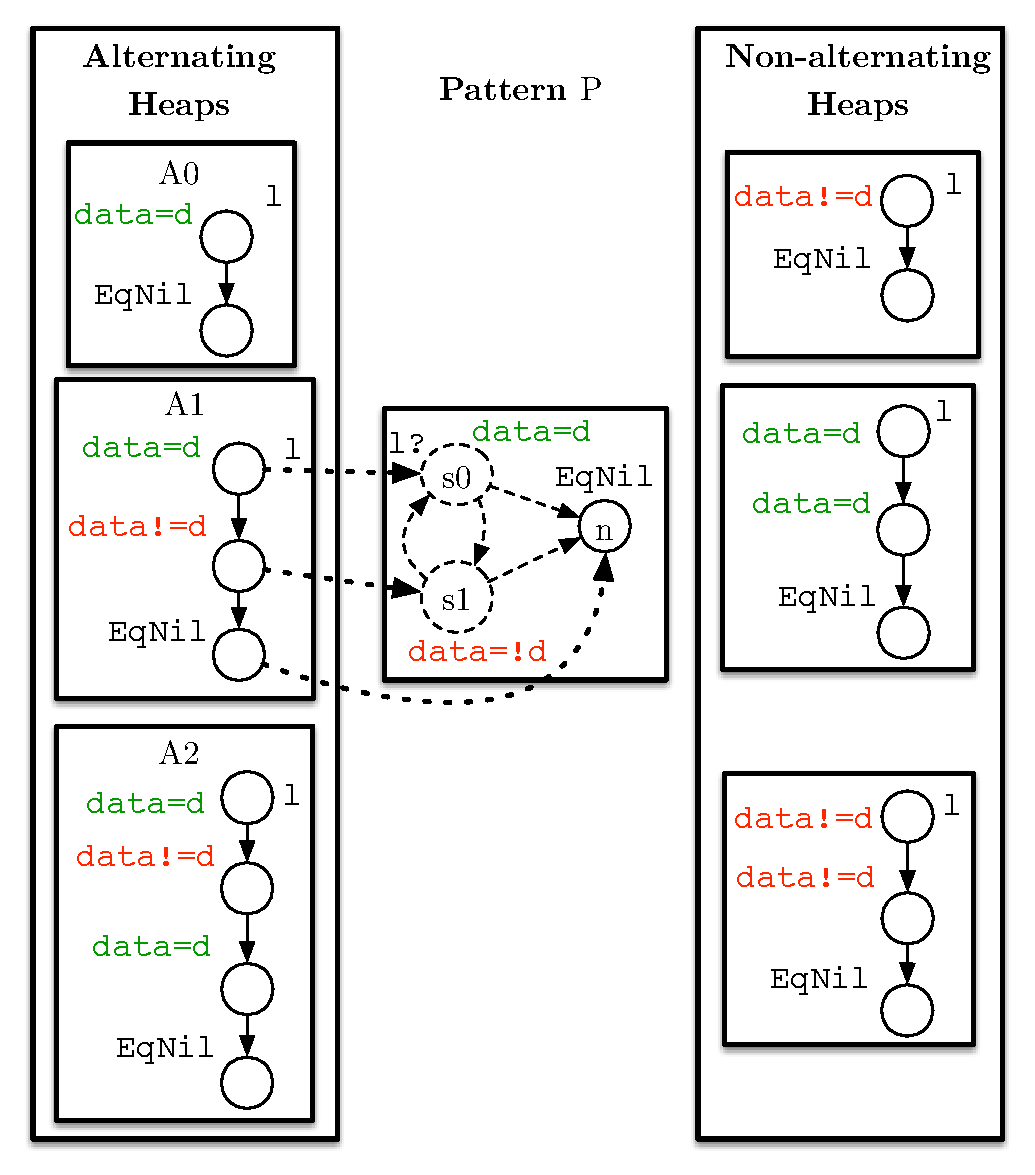
\includegraphics[width=\linewidth]{fig/exs.pdf}
  \caption{Sets of alternating heaps and non-alternating heaps of
    \altlist (\autoref{sec:ex-program}), depicted as graphs, and a
    heap pattern that matches each of the alternating heaps and none
    of the non-alternating heaps.
    %
    The labels of each node $n$ are written adjacent to the node in a heap
    graph are written adjacent to $n$;
    %
    some label values are colored for clarity.
    %
    Each edge is implicitly labeled with the field name \nextnm.
    %
    Each summary node of the pattern $\patnm$ is dashed, each
    indefinite node label is followed by a question mark, and each
    indefinite edge with an indefinite label is dashed.
    %
    The dash-dotted lines from heap $A_1$ to $\patnm$ depict a matching
    from $A_1$ to $\patnm$.
    % 
  }
  \label{fig:alt-pattern}
\end{figure}

% Example: concrete heaps.
\begin{ex}
  \label{ex:concrete-heaps}
  \autoref{fig:alt-pattern} depicts distinct sets of graphs of heaps
  in \altlist states that (1) are alternating and (2) are not
  alternating (for now, ignore the pattern $P$ with dashed nodes and
  edges in the center of \autoref{fig:alt-pattern}).
  %
  The alternating heaps depicted consist of the alternating heaps with
  one to three non-nil cells.
  %
  The non-alternating heaps depicted consist of three non-alternating
  heaps with one to two non-nil cells.
\end{ex}

% Pattern as graph:
Each pattern is a graph in which nodes and edges are labeled from the
space of annotations as the labels on the nodes and edges of heap
graphs.
%
However, a pattern graph may also contain \emph{summary nodes} and
\emph{indefinite labelings}.
%
A heap graph $H$ is \emph{matched} by a pattern graph $P$ if there is
a mapping $\matchnm$ from the nodes of $H$ to the nodes of $P$ such
that:
%
\begin{enumerate}
\item 
  % Multiple cells only go to a summary node.
  If multiple nodes of $H$ are matched by a node $n$ of $P$, then $n$
  is a summary node.
\item 
  % Preserves node labelings.
  For each node $\nodenm$ of $H$, if $\nodenm$ is labeled with label $L$,
  then $\matchnm(\nodenm)$ is either definitely or indefinitely labeled
  with $L$.
  %
  If $\nodenm$ is not labeled with label $L$, then $\matchnm(\nodenm)$
  is either definitely not labeled or indefinitely labeled with $L$.
\item 
  % Preserves 
  For all nodes $m$ and $n$ of $H$, if there is an edge from $m$ to
  $n$ labeled with field $\fieldnm$, then there is an edge from
  $\matchnm(m)$ to $\matchnm(n)$ either definitely or indefinitely
  labeled with $\fieldnm$.
  %
  If there is no edge from $m$ to $n$ labeled with $\fieldnm$, then
  either there is no edge from $\matchnm(m)$ to $\matchnm(n)$ labeled
  with $\fieldnm$ or there is an edge from $\matchnm(m)$ to
  $\matchnm(n)$ indefinitely labeled with $\fieldnm$.
\end{enumerate}

% Example: walk through the heap graphs and patterns in the example.
\begin{ex}
  \label{ex:heap-pats}
  % Walk through the pattern.
  The heap pattern $\patnm$ depicted in \autoref{fig:alt-pattern}
  matches exactly the alternating heaps of \altlist.
  %
  A matching from the second alternating heap $A_1$ in
  \autoref{fig:alt-pattern} to $\patnm$ is depicted with dotted edges
  from the nodes of the heap to the nodes of the pattern.
  %
  Because $\patnm$ matches each of the alternating heaps and none of
  the non-alternating heaps in \autoref{fig:alt-pattern}, we say that
  $\patnm$ \emph{distinguishes} the alternating and non-alternating
  heaps.
\end{ex}

% Walk through the proof structure for the example.
\subsection{A proof structure for low-level heap programs}
\label{sec:ex-tree}
% Walk through the example.
\altlist demonstrates that proving that some programs satisfy each of
their assertions, which are defined purely over local variables, may
still sometimes require a verifier to find invariants over the entire
structure of the program heap.
%
In particular, in order to prove that \altlist always satisfies its
assertion at a line 12, a verifier must prove that at line 5, the heap
always holds an alternating list.

% Describe the proof structure in general.
\verifier attempts to construct proofs that are represented as a
partial prefix-tree (i.e., an \emph{unwinding tree}) of the program's
control paths~\cite{mcmillan06}.
% Nodes:
Each node in the tree models an occurrence of a control location in a
program path, and each edge in the tree models a step of execution of
the program over a sequence of non-branching instructions.
% Edges.
Each node $n$ is thus identified by a sequence of instructions
$\instrs_n$ that the program must execute to reach the node, and is
annotated with an \emph{invariant}, represented as a heap pattern
(\autoref{sec:ex-patterns}) that is satisfied by all states reached
after the program executes $\instrs_n$.

% Conditions on tree as a valid proof.
An unwinding tree $T$ is a proof that a given error location $\errloc$
is unreachable in any run of a program $P$ if:
%
\begin{enumerate}
%
\item 
  % Condition on initial states.
  The initial heap of $P$ satisfies the invariant at the root of $T$.
\item
  % Adjacent nodes model the semantics of the program.
  For each edge $(m, n)$ in $T$, the invariant at $m$ and the
  semantics of the instructions modeled by the edge $(m, n)$ imply the
  invariant at $n$.
\item
  % Condition on error nodes.
  Each node in $T$ that models $\errloc$ is annotated with an
  invariant that is not satisfied by any program state.
\item
  % Covering.
  Each leaf $l$ that models control location $\locnm$ of $T$ either
  models a terminal control location of $P$, or is \emph{covered} by
  another node of $T$ that models $\locnm$, and is annotated with a
  weaker invariant than the invariant of $l$.
\end{enumerate}
%
If a leaf $l$ is covered by node $n$, the intuitively the proof tree
need not be further expanded from $l$, because any proof tree rooted
at $n$, which is a proof of safety for all paths with prefix
$\instrs_n$, is a valid proof of safety for all paths with prefix
$\instrs_l$.

% Figure with an annotated unwinding tree.
\begin{figure}
  \centering
  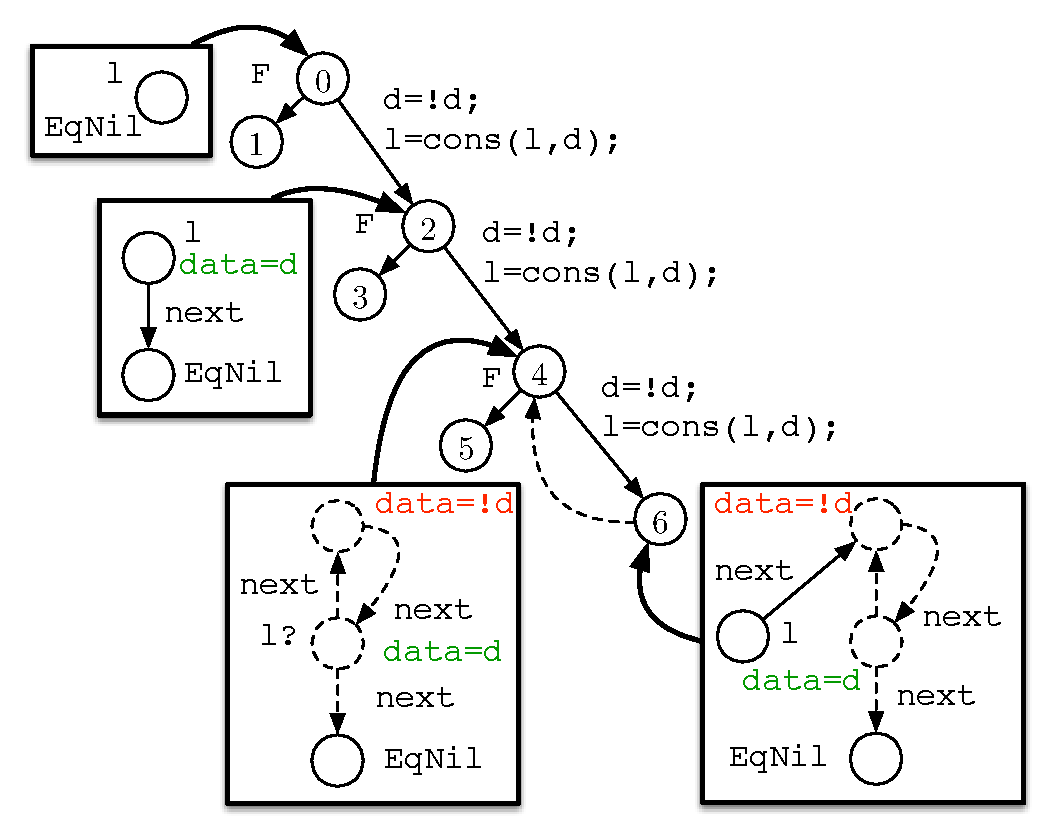
\includegraphics[width=\linewidth]{fig/alt-tree.pdf}
  \caption{The prefix of an unwinding tree $\treenm$ that proves that
    no run of \altlist violates its assertion.
    %
    Edge tree edge is annotated with the instruction sequence that it
    simulates, and each node is annotated with its pattern invariant.
  }
  \label{fig:alt-unwinding}
\end{figure}

% Walk through the unwinding tree for the example program.
\begin{ex}
  \label{ex:alt-list-pf}
  % Give an overview of the example.
  \autoref{fig:alt-unwinding} depicts a prefix tree $T$ of an
  unwinding tree that proves that \altlist always satisfies the
  assertion at line 12.
  %
  $T$ models runs of \altlist that execute \consloop most three times.
  % Talk about nodes.
  Nodes $0$, $2$, $4$, and $6$ model states of \altlist when control
  is at the loop head, and
  %
  nodes $1$, $3$, and $5$ model states of \altlist when control exits
  \consloop.
  % Talk about edges.
  Each edge of $T$ is annotated with the sequence of instructions in
  \altlist that it models.
  %
  Each node $n$ of $T$ is annotated with a heap pattern
  (\autoref{sec:ex-patterns}) that over-approximates the set of heaps
  reachable by executing $\instrs_n$.
  %
  Node $6$ is covered by node $4$ because the pattern at node $6$ is
  entailed by the pattern at node $4$.
  %
  Thus, tree $T$ can be expanded into a complete tree that proves the
  safety of $P$ by expanding $T$ from only leaf nodes $1$, $3$, and
  $5$, not from leaf node $6$.
\end{ex}

% Define heap games.
\subsection{Learning heap patterns as a game}
\label{sec:ex-heap-games}
\BH{this section needs to be updated to match the new formulation}
% Summary:
The key observation behind the design of \verifier is that any pair of
disjoint sets of heaps $\posheaps$ and $\negheaps$ defines a natural
game, in which the objective for one player is to learn a pattern that
distinguishes $\posheaps$ from $\negheaps$.
% Introduce the key observation: learning is a game.
In particular, let an \emph{inductive pattern synthesizer} be an
oracle that takes as input a finite set of positive heaps $\posheaps$
and negative heaps $\negheaps$, and returns a heap pattern that is
matched by each heap $\posheaps$ and no heap in $\negheaps$.
%
The synthesizer's goal in the game is to synthesize a heap pattern
that distinguishes $\posheaps$ and $\negheaps$, without direct access
to $\posheaps$ and $\negheaps$.
%
The state of the game consists of finite subsets of \emph{revealed}
$\posheaps_0 \subseteq \posheaps$ and revealed $\negheaps \subseteq
\negheaps$, and a pattern $\patnm$ generated by the synthesizer that
distinguishes $\posheaps_0$ from $\negheaps_0$.
%
In each play, if the inductive pattern synthesizer has not won, then
the pattern verifier reveals either a heap in $\posheaps$ not matched
$\patnm$ or a heap in $\negheaps$ that is matched by $\patnm$.
%
The inductive pattern synthesizer then generates a new pattern that
must match all revealed patterns in $\posheaps$ and no revealed
patterns in $\negheaps$.
% Example: game for line 5.
\begin{ex}
  \label{ex:alt-list-game}
  For \altlist, the reachable heaps and heaps that lead to an
  assertion violation from line $\gamenm_5$ (i.e., the alternating
  heaps and non-alternating heaps) define a pattern-synthesis game
  $\gamenm_5$.
  %
  One valid play of the game with an inductive pattern synthesizer
  $\oraclenm_5$ from a game state consisting of no revealed positive
  heaps and the non-alternating heaps in \autoref{fig:alt-pattern} as
  revealed negative heaps is as follows:
  %
  (1) $\oraclenm_5$ plays the pattern that annotates node $0$ in
  \autoref{fig:alt-unwinding};
  %
  (2) the pattern verifier reveals heap $A_1$ in
  \autoref{fig:alt-pattern};
  % 
  (3) $\oraclenm_5$ plays the pattern that annotates node $2$ in
  \autoref{fig:alt-unwinding};
  %
  (4) the pattern verifier reveals heap $A_2$ in
  \autoref{fig:alt-pattern};
  %
  (5) $\oraclenm_5$ plays the pattern that annotates node $4$ in
  \autoref{fig:alt-unwinding} (i.e., pattern $P$ in
  \autoref{fig:alt-pattern}), and wins the game.
\end{ex}

% Walk through how we infer invariants for the example.
\subsection{From game strategies to program proofs}
\label{sec:ex-infer}
%
The main result of our work is that while the problem of verifying
heap-manipulating programs is undecidable, it can be reduced to
winning a finite set of pattern-synthesis games.
%
The primary difficulty in constructing an unwinding tree $T$ that
proves the safety of a program is in inferring patterns for the nodes
of $T$ that are (1) sufficiently strong enough to prove that each path
of $T$ to an error node is infeasible but (2) sufficiently weak that
they can cover the patterns of sufficiently many leaf nodes to bound
the set of program paths that must be modeled.
%
For the example of \altlist, the pattern on node $4$ of the unwinding
tree in \autoref{fig:alt-unwinding} satisfies both of these criteria;
%
however, in general the problem of inferring sufficient patterns is
undecidable, and to date, there are not general-purpose analyses that
can infer such invariants for practical programs.

% Context: interpolation works for non-graphical data.
In settings where it is not critical to infer properties of the
program's entire heap, it is sufficient to infer invariants for an
unwinding tree by obtaining an \emph{interpolant}~\cite{mcmillan06}
for each node $n$ of two formulas describing (1) states reachable by
executing the instruction sequence of $n$ from the beginning of the
program and (2) states from which $n$ reaches an error.
% 
However, interpolation-based approaches must infer interpolants as
formulas in a theory for which the problem of constructing an
interpolant is decidable, typically the combined theory of linear
arithmetic, uninterpreted functions, and arrays (\liufa).
%
Unfortunately, formulas in such theories cannot naturally describe
sets of heaps with arbitrarily many cells, such as the set of
alternating heaps of \altlist (\autoref{sec:ex-program}).

% Our assumption: hypothesis
In this work, we explore under what conditions a verifier can
efficiently learn heap patterns that are sufficient invariants for
proving the correctness of a program, under the assumption that the
verifier can query an oracle that can efficiently win a class of the
heap-learning games described in \autoref{sec:ex-heap-games}.
%
% Example heaps:
\begin{ex}
  \label{ex:alt-list-pat-syn}
  % Introduce problem:
  Suppose that \verifier has constructed the unwinding tree depicted
  in \autoref{fig:alt-unwinding}, and must choose a pattern with which
  to annotate node $4$, which models line 5 of \altlist.
  %
  \verifier could choose a pattern $P$ that only distinguishes between
  alternating and non-alternating lists of length less than or equal
  to two.
  %
  However, $P$ is, intuitively too strong an invariant in that it
  cannot cover any valid annotation of node $6$.

  % Alternative: choosing patterns as game solutions.
  Alternatively, if \verifier plays the game $\gamenm_5$ as pattern
  verifier against the pattern synthesizer $\oraclenm_5$
  (\autoref{ex:alt-list-game}), and annotates node $4$ with the
  winning pattern played by $\oraclenm_5$ (as depicted in
  \autoref{fig:alt-unwinding}), then \verifier can construct an
  unwinding tree that proves the safety of \altlist.
\end{ex}

% State our main result in formally.
The main result that we present in this paper is that for a given
program $\prognm$, if our program verifier \verifier has access to an
inductive pattern synthesizer that wins a game defined analogously to
the game $\gamenm_5$ defined for line 5 of \autoref{fig:alt-list}
(\autoref{ex:alt-list-game}) for each control location of $\prognm$,
then \verifier verifies $\prognm$ successfully.

%%% Local Variables: 
%%% mode: latex
%%% TeX-master: "p"
%%% End: 


\chapter{Background}
% Background: give technical background
% \section{Background}
\label{ch:background}

In this section, we define the formalize requirements for lazy interpolation-based model checking, based on \cite{mcmillan06}. This applies to the standard domain of model checking for programs that don't use heap memory, and we'll extend it to heap-manipulating programs later.

We will use standard first-order logic (FOL) and the notation $\mathcal{L}(\Sigma)$ to denote the set of well-formed formulas (\textit{wffs}) of FOL over a vocabulary $\Sigma$ of non-logical symbols. For a given formula or set of formulas $\phi$ we will use $\mathcal{L}(\phi)$ to denote \textit{wffs} over the vocabulary of $\phi$.

For every non-logical symbol $s$, we presume the existence of a unique symbol $s'$ (that is, $s$ with one prime added). We think of $s$ with $n$ primes added as representing the value of $s$ at $n$ time units in the future. For any formula or term $\phi$, we will use the notation $\phi^{\langle n \rangle}$ to denote the addition of $n$ primes to every symbol in $\phi$ (meaning $\phi$ at $n$ time units in the future). For any set $\Sigma$ of symbols, let $\Sigma'$ denote $\{ s' | s \in \Sigma \}$ and $\Sigma^{\langle n \rangle}$ denote $\{ s^{\langle n \rangle} | s \in \Sigma \}$.

\section{Modeling Programs}
\label{sec:modeling-programs}

We use FOL formulas to characterize programs. To this end, let $S$, the state vocabulary, be a set of individual variables and uninterpreted $n$-ary functional and propositional constants. A \textit{state formula} is a formula in $\mathcal{L}(S)$ (which may also include various interpreted symbols, such as $=$ and $+$). A \textit{transition formula} is a formula in $\mathcal{L}(S \cup S')$.

For our purposes, a \textit{program} is a tuple $(\Lambda, \Delta, l_i, l_f)$, where $\Lambda$ is a finite set of program locations, $\Delta$ is a set of $actions$, $l_i \in \Lambda$ is the initial location and $l_f \in \Lambda$ is the error location. An $action$ is a triple $(l, T, m)$, where $l,m \in \Lambda$ are respectively the entry and exit locations of the action, and $G$ is a transition formula. A $path$ $\pi$ of a program is a sequence of transitions of the form $(l_0, T_0, l_1)(l_1, T_1, l_2) \cdots (l_{n-1}, T_{n-1}, l_n)$. The path is an \textit{error path} when $l_0 = l_1$ and $l_n = l_f$. The unfolding $\mathcal{U}(\pi)$ of path $\pi$ is the sequence of formulas $T_0^{\langle 0 \rangle}, \cdots, T_{n-1}^{\langle n-1 \rangle}$, that is, the sequence of transition formulas $T_0, \cdots, T_{n-1}$, with each $T_i$ shifted $i$ time units into the future.

We will say that path $\pi$ is $feasible$ when $\bigwedge \mathcal{U}(\pi)$ is consistent. We can think of a model of $\bigwedge \mathcal{U}(\pi)$ as a concrete program execution, assigning a value ot every program variable at every time $0, \cdots, n-1$. A program is said to be $safe$ when every error path of the program is infeasible. An \textit{inductive invariant} of a program is a map $I : \Lambda \rightarrow \mathcal{L}(S)$, such that $I(l_i) \equiv \true$ and for every action $(l, T, m) \in \Delta$, $I(l) \wedge T$ implies $I(m)'$. A \textit{safety invariant} of a program is an inductive invariant such that $I(l_f) \equiv \false$. Existence of a safety invariant of a program implies that the program is safe.

To simplify the presentation of algorithms, we will assume that every location has at least one outgoing action. This can be made true without affecting program safety by adding self-loops.

\section{Interpolants from Proofs}
\label{sec:interpolants-from-proofs}

Given a pair of formulas $(A,B)$, such that $A \wedge B$ is inconsistent, an \textit{interpolant} for $(A,B)$ is a formula $\hat{A}$ with the following properties:

\begin{itemize}
  \item $A$ implies $\hat{A}$
  \item $\hat{A} \wedge B$ is unsatisfiable, and
  \item $\hat{A} \in \mathcal{L}(A) \cap \mathcal{L}(B)$
\end{itemize}

The Craig Interpolation lemma \cite{craig1957} states that an interpolant always exists for inconsistent formulas in FOL. To handle program paths, this idea can be generalized to sequences of formulas. That is, given a sequence of formulas $\Gamma = A_1, \cdots , A_n$, we say that $\hat{A_0},\cdots, \hat{A_n}$ is an \textit{interpolant} for $\Gamma$ when

\begin{itemize}
  \item $\hat{A_0} = \true$ and $\hat{A_n} = \false$ and,
  \item for all $1 \leq i \leq n, \hat{A_{i-1}} \wedge A_i$ implies $\hat{A_i}$ and
  \item for all $1 \leq i < n, \hat{A_i} \in (\mathcal{L}(A_1 \cdots A_i) \cap \mathcal{L}(A_{i+1}\cdots A_n))$
\end{itemize}

That is, the $i$-th element of the interpolant is a formula over the common vocabulary of the prefix $A_1 \cdots A_i$ and the suffix $A_{i+1} \cdots A_n$, and each interpolant implies the next, with $A_i$. If $\Gamma$ is quantifier-free, we can derive a quantifier-free interpolant for $\Gamma$ from a refutation of $\Gamma$, in certain interpreted theories \cite{mcmillan05}.

\section{Program Unwindings}

We now give a definition of a program unwinding, and describe an algorithm to construct a complete unwinding using interpolants. For two vertices $v$ and $w$ of a tree, we will write $w \sqsubset v$ when $w$ is a proper ancestor of $v$.

% define program unwinding
\begin{defn}
  \label{defn:prog-unwinding}
  An unwinding of a program $\mathcal{A} = (\Lambda, \Delta, l_i, l_f)$ is a quadruple $(V, E, M_v, M_e)$, where $(V, E)$ is a directed tree rooted at $\epsilon$, $M_v : V \rightarrow \Lambda$ is the vertex map, and $M_e : E \rightarrow \Delta$ is the edge map, such that:

  \begin{itemize}
    \item $M_v(\epsilon) = l_i$
    \item for every non-leaf vertex $v \in V$, for every action $(M_v(v), T, m) \in \Delta$, there exists an edge $(v,w) \in E$ such that $M_v(w) = m$ and $M_e(v,w) = T$
  \end{itemize}
\end{defn}

% define labeled program unwinding
\begin{defn}
  \label{defn:labeled-prog-unwinding}
  A labeled unwinding of a program $\mathcal{A} = (\Lambda, \Delta, l_i, l_f)$ is a triple $(U, \psi, \rhd)$, where

  \begin{itemize}
    \item $U = (V, E, M_v, M_e)$ is an unwinding of $\mathcal{A}$
    \item $\psi : V \rightarrow \mathcal{L}(S)$ is called the vertex labeling, and
    \item $\rhd \subseteq V \times V$ is called the covering relation
  \end{itemize}

  A vertex $v \in V$ is said to be covered iff there exists $(w,x) \in \rhd$ such that $w \sqsubseteq v$. The unwinding is said to be safe iff, for all $v \in V$, $M_v(v) = l_f$ implies $\psi(v) \equiv \false$. It is complete iff every leaf $v \in V$ is covered.
\end{defn}

% define well-labeled program unwinding
\begin{defn}
  \label{defn:well-labeled-prog-unwinding}
  A labeled unwinding $(U, \psi, \rhd)$ of a program $\mathcal{A} = (\Lambda, \Delta, l_i, l_f)$, where $U = (V, E, M_v, M_e)$, is said to be well-labeled iff:

  \begin{itemize}
    \item $\psi(\epsilon) \equiv \true$, and
    \item for every edge $(v,w) \in E$, $\psi(v) \wedge M_e(v,w)$ implies $\psi(w)'$, and
    \item for all $(v,w) \in \rhd$, $\psi(v) \Rightarrow \psi(w)$, and $w$ is not covered
  \end{itemize}

  A vertex $v \in V$ is said to be covered iff there exists $(w,x) \in \rhd$ such that $w \sqsubseteq v$. The unwinding is said to be safe iff, for all $v \in V$, $M_v(v) = l_f$ implies $\psi(v) \equiv \false$. It is complete iff every leaf $v \in V$ is covered.
\end{defn}

Notice that, if a vertex is covered, all its descendants are also covered. Moreover, we do not allow a covered vertex to cover another vertex.

\begin{thm}
  If there exists a safe, complete, well-labeled unwinding of program $\mathcal{A}$, then $\mathcal{A}$ is safe.
\end{thm}

This is Theorem 1 from \cite{mcmillan06}.

% describe the standard Impact algorithm
\section{Impact Algorithm}
\label{sec:impact-algorithm}
%

This section describes a semi-algorithm from \cite{mcmillan06}, for building a complete, safe, well-labeled unwinding of a program. The algorithm terminates if the program is unsafe, but may not terminate if it is safe (which is expected, since program safety is undecidable). A non-deterministic procedure with three basic steps is outlined here. The three steps are

\begin{itemize}
  \item \expand, which generates the successors of a leaf vertex (\autoref{alg:expand})
  \item \refine, which refines the labels along a path, labeling an error vertex $\false$ (\autoref{alg:refine})
  \item \cover, which expands the covering relation (\autoref{alg:cover})
\end{itemize}

The interpolant in \refine can be generated from a refutation of $\mathcal{U}(\pi)$ by the method of \cite{mcmillan05}. Each of the three steps preserves well-labeledness of the unwinding. To make the unwinding safe, we have to only apply \refine to every error vertex. When none of the three steps can produce any change, the unwinding is both safe and complete, so we know that the original program is safe.
To build a well-labeled unwinding, a strategy is required, for applying the three unwinding rules. The most difficult question is when to apply \cover. Covering one vertex can result in uncovering others. Thurs, applying \cover non-deterministically may not terminate.

\subsection{Termination}
The \impact algorithm works by repeated applications of \expand, \cover, and \refine. When any of the three procedures don't cause any change in the unwinding tree, the algorithm terminates. The order of application matters, and the \unwind algorithm in \cite{mcmillan06} describes a systematic way of applying the three procedures. Forced covering (calling \cover on all nodes of a path after a \refine step) also serves as an optimization. All of these ideas apply directly to the case of heap-manipulating programs.

\begin{algorithm}[ht]
  % Declare functions
  \SetKwFunction{procexpand}{EXPAND}

  % Declare sub-program markers.
  \SetKwProg{myproc}{Procedure}{}{}

  % expand
  \myproc{\procexpand{$v \in V$}:}{
    %
    \If{$v$ is an uncovered leaf}{
        \ForEach{action $(M_v(v),T,m) \in \Delta$}{
        add a new vertex $w$ to $V$ and a new edge $(v,w)$ to $E$; \\
        set $M_v(w) \leftarrow m$ and $\psi(w) \leftarrow \true$; \\
        set $M_e(v,w) \leftarrow T$;
      }
    }
  }
  \caption{$\expand$: takes as input a vertex $v \in V$ and expands the control flow graph based on all actions available at that vertex.}
  \label{alg:expand}
\end{algorithm}

\begin{algorithm}[ht]
  % Declare functions
  \SetKwFunction{procrefine}{REFINE}

  % Declare sub-program markers.
  \SetKwProg{myproc}{Procedure}{}{}

  % expand
  \myproc{\procrefine{$v \in V$}:}{
    %
    \If{$M_v(v) = l_f$ and $\psi(v) \not\equiv \false$}{
      let $\pi = (v_0, T_0, v_1) \cdots (v_{n-1}, T_{n-1}, v_n)$ be the unique path from $\epsilon$ to $v$ \\
      \eIf{$\mathcal{U}(\pi)$ has an interpolant $\hat{A_0},\cdots,\hat{A_n}$}{
          \For{$i = 0 \cdots n$}{
          let $\phi = \hat{A}_i^{\langle -i \rangle}$ \\
          \If{$\psi(v_i) \nvDash \phi$}{
            remove all pairs $(\cdot, v_i)$ from $\rhd$; \\
            set $\psi(v_i) \leftarrow \psi(v_i) \land \phi$;
          }
        }
      }
      {
        abort (program is unsafe)
      }
    }
  }
  \caption{$\refine$: takes as input a vertex $v \in V$ at an error location and tags the path from root to $v$ with invariants.}
  \label{alg:refine}
\end{algorithm}

\begin{algorithm}[ht]
  % Declare functions
  \SetKwFunction{proccover}{COVER}

  % Declare sub-program markers.
  \SetKwProg{myproc}{Procedure}{}{}

  % expand
  \myproc{\proccover{$v, w \in V$}:}{
    %
    \If{$v$ is uncovered and $M_v(v) = M_v(w)$ and $v \nvDash w$}{
      \If{$\psi(v) \vDash \psi(w)$}{
        add $(v,w)$ to $\rhd$; \\
        delete all $(x,y) \in \rhd$, s.t. $v \sqsubseteq y$;
      }
    }
  }
  \caption{$\cover$: takes as input vertices $v, w \in V$ and attempts to cover $v$ with $w$.}
  \label{alg:cover}
\end{algorithm}

%%% Local Variables:
%%% mode: latex
%%% TeX-master: "p"
%%% End:


\chapter{Heap Patterns}
% Describe heap patterns

\section{Heap Patterns}
\label{sec:heap-patterns}
%
In this section, we define a standard language that performs low-level
memory operations to update linked data structures
(\autoref{sec:lang}).
%
We then review definitions of three-valued structures introduced in
previous work~\cite{sagiv02}, which we use to formulate patterns over
program heaps (\autoref{sec:patterns}).

% Define a toy imperative language.
\subsection{Language Definition}
\label{sec:lang}
%
In this section, we define the syntax (\autoref{sec:syntax}) and
semantics (\autoref{sec:semantics}) of our subject language \lang.

% Define the language syntax.
\subsubsection{Syntax}
\label{sec:syntax}
% Define the syntax of a program.
\begin{figure}
  \centering
  \begin{align}
    % A program is a sequence of statements.
    \lang \assign & (\locs: \instrs)^{*} \label{line:prog} \\
    % A statement is a predicate instruction or a heap instruction.
    \instrs \assign & \predinstr\ |\ \heapinstr \label{line:instrs} \\
    % A predicate instruction:
    \predinstr \assign &
    % updates predicates according to an operation.
    \predvars \assign \predvars\ \predops\ \predvars
    %
    \label{line:bool-op} \\
    % or tests equalities of heap variables,
    |\ & \predvars \assign (\heapvars = \heapvars)
    %
    \label{line:test-eq} \\
    % or branches.
    |\ & \branch\ \predvars, \locs, \locs \label{line:branch} \\
    % A heap instruction: allocates a new cell:
    \heapinstr \assign & \heapvars \assign \alloc()
    %
    \label{line:alloc} \\
    % or a copy,
    |\ & \heapvars \assign \heapvars \label{line:copy} \\
    % or a load,
    |\ & \heapvars \assign \heapvars \select \fields
    %
    \label{line:load} \\
    % or a store.
    |\ & \heapvars \select \fields \assign \heapvars
    %
    \label{line:store}
  \end{align}
  \caption{Syntax of heap-updating programs, $\lang$.
    %
    The spaces of control locations, predicate variables, heap
    variables, and fields are denoted $\locs$, $\predvars$,
    $\heapvars$, and $\fields$, respectively.
  }
  \label{fig:syntax}
\end{figure}

% Walk through the full syntax of programs.
A \lang program is a sequence of instructions that operate on a fixed
set of predicate variables and pointers to heap objects.
%
The syntax of \lang is given in \autoref{fig:syntax} for fixed finite
sets of control locations $\locs$, predicate variables $\predvars$,
heap variables $\heapvars$, and heap fields $\fields$.
%
A program is a sequence of instruction, each labeled with a control
location (\autoref{line:prog}).
%
An instruction either updates the program's predicate variables or
heap variables (\autoref{line:instrs}).
%
An instruction that updates predicate variable either stores in a
predicate variable the result of a Boolean operation
(\autoref{line:bool-op}),
%
an equality test on heap cells (\autoref{line:test-eq}),
%
or branches control based on the value in a predicate variable
(\autoref{line:branch}).
%
An instruction that updates heap variables either allocates a new heap
cell (\autoref{line:alloc}),
%
copies the heap cell from one pointer variable to another
(\autoref{line:copy}),
%
loads a heap cell into a pointer variable (\autoref{line:load}),
%
or stores a heap cell as a child of a cell in a pointer variable
(\autoref{line:store}).

% Define the control-flow graph.
For each program $P \in \lang$, the control-flow graph of $P$,
$\cfg_P \subseteq \locs \times \instrs \times \locs$, is defined in
the standard way.


\chapter{\verifier: The Heap Impact Algorithm}
% describe the modification of the Impact algorithm for heaps

% describe the standard Impact algorithm
\section{Heap Impact Algorithm}
\label{sec:heap-impact-algorithm}
%

Building on top of the framework defined in \autoref{sec:background}, \autoref{sec:impact-algorithm}, and \autoref{sec:heap-patterns}, we can now modify the \impact algorithm to work for heap-manipulating programs. In this section, we first define the three steps of \impact, that is \expand, \cover, and \refine. Then we describe an invariant-learning procedure that retrieves patterns from an Oracle, thereby completing the description of the algorithm.

\begin{algorithm}[ht]
  % Declare functions
  \SetKwFunction{procexpand}{EXPAND}

  % Declare sub-program markers.
  \SetKwProg{myproc}{Procedure}{}{}

  % expand
  \myproc{\procexpand{$v \in V$}:}{
    %
    \If{$v$ is an uncovered leaf}{
        \ForEach{action $(M_v(v),T,m) \in \Delta$}{
        add a new vertex $w$ to $V$ and a new edge $(v,w)$ to $E$; \\
        set $M_v(w) \leftarrow m$ and $\psi(w) \leftarrow 1_D$; \\
        set $M_e(v,w) \leftarrow T$;
      }
    }
  }
  \caption{$\expand$: takes as input a vertex $v \in V$ and expands the control flow graph based on all actions available at that vertex.}
  \label{alg:heap-expand}
\end{algorithm}

\begin{algorithm}[ht]
  % Declare functions
  \SetKwFunction{procrefine}{REFINE}

  % Declare sub-program markers.
  \SetKwProg{myproc}{Procedure}{}{}

  % expand
  \myproc{\procrefine{$v \in V$}:}{
    %
    \If{$M_v(v) = l_f$ and $\psi(v) \not\equiv (\false, 0_D)$}{
      let $\pi = (v_0, T_0, v_1) \cdots (v_{n-1}, T_{n-1}, v_n)$ be the unique path from $\epsilon$ to $v$ \\
      let $\hat{A_0},\cdots,\hat{A_n}$ = \seplearner($\mathcal{U}(\pi)$) \\
      \eIf{$\hat{A_0},\cdots,\hat{A_n}$ is a valid interpolant}{
          \For{$i = 0 \cdots n$}{
          let $\phi = \hat{A}_i^{\langle -i \rangle}$ \\
          \If{$\psi(v_i) \nvDash \phi$}{
            remove all pairs $(\cdot, v_i)$ from $\rhd$; \\
            set $\psi(v_i) \leftarrow \psi(v_i) \land \phi$;
          }
        }
      }
      {
        abort (program is unsafe)
      }
    }
  }
  \caption{$\refine$: takes as input a vertex $v \in V$ at an error location and tags the path from root to $v$ with invariants.}
  \label{alg:heap-refine}
\end{algorithm}

\begin{algorithm}[ht]
  % Declare functions
  \SetKwFunction{proccover}{COVER}

  % Declare sub-program markers.
  \SetKwProg{myproc}{Procedure}{}{}

  % expand
  \myproc{\proccover{$v, w \in V$}:}{
    %
    \If{$v$ is uncovered and $M_v(v) = M_v(w)$ and $v \nvDash w$}{
      \If{$\psi(v) \vDash \psi(w)$}{
        add $(v,w)$ to $\rhd$; \\
        delete all $(x,y) \in \rhd$, s.t. $v \sqsubseteq y$;
      }
    }
  }
  \caption{$\cover$: takes as input vertices $v, w \in V$ and attempts to cover $v$ with $w$.}
  \label{alg:heap-cover}
\end{algorithm}

\subsection{Postcondition Transforms for Heap Operations}
TODO: This section needs to be completed.

% define labeled program unwinding
\begin{defn}
  \label{defn:heap-post-transforms}
  We define the operator $\post$, which computes the strongest postcondition for a given heap pattern, and action. That is $\post : \heappats \times \mathcal{T} \to \heappats$, where $\mathcal{T}$ is the set of all actions.
\end{defn}

The formal rules for computing $\post$ for each individual action are presented in \autoref{fig:post-transforms}. (TODO)

\subsection{Learning Invariants from Positive and Negative Examples}

We note in \autoref{alg:heap-refine} the procedure \seplearner is used, which is the core component of making \impact work for heap-manipulating programs. In this section, we describe this algorithm.

We defined the notion of interpolants in \autoref{sec:interpolants-from-proofs}, and the same applies to \seplearner, which is described in \autoref{alg:invlearner}.

\begin{algorithm}[ht]
  % Declare functions
  \SetKwFunction{procinvlearner}{INVLEARNER}

  % Declare sub-program markers.
  \SetKwProg{myproc}{Procedure}{}{}

  % expand
  \myproc{\procinvlearner{$\mathcal{U}(\pi)$}:}{
    %
    \If{$v$ is uncovered and $M_v(v) = M_v(w)$ and $v \nvDash w$}{
      \If{$\psi(v) \vDash \psi(w)$}{
        add $(v,w)$ to $\rhd$; \\
        delete all $(x,y) \in \rhd$, s.t. $v \sqsubseteq y$;
      }
    }
  }
  \caption{$\seplearner$: takes as input an unfolding $\mathcal{U}(\pi)$ of path $\pi$ and attempts to find an invariant for it.}
  \label{alg:invlearner}
\end{algorithm}

While \seplearner is the higher level procedure to find an interpolant, it uses a sub-procedure called <NAME TODO> as a feedback loop with the Oracle, to accept candidate heap patterns that can be used to construct an interpolant.

\chapter{User Interface to a Human Oracle}
% describe user interface
% \section{Interface with the Oracle}
\label{ch:interface-oracle}

In this chapter, we describe one implementation of the Oracle. In \autoref{alg:newcandidate}, the candidate is obtained as $C = \mathcal{O}(H_i^{+}, H_i^{-})$. The Oracle $\mathcal{O}$ considers two sets of concrete heaps $H_i^{+}$ and $H_i^{-}$, and returns a candidate pattern $C$ which is then evaluated. After the evaluation, it is either accepted, or needs to be further refined, in which case $H_i^{+}$ or $H_i^{-}$ are updated, and a new query is submitted to the Oracle. This process repeats until a suitable candidate is found for the current vertex in the program unwinding.

\section{Human as an Oracle}
Human beings are good at finding patterns in several types of spatial data. This fact has been utilized for crowdsourcing the harder parts of several difficult technical problems \cite{wenchao2012, verigames, eyewire}. The important challenges are to identify steps in the problem where human insight is critical, find ways to transform these steps into tasks that non-expert humans can perform, and combine the results to resolve those steps in the solution. In our problem of verifying heap-manipulating programs, the goal of the Oracle is to provide heap patterns that can be used to generate interpolants, which are then used for verification. Finding these interpolants automatically is a difficult step in program verification, while checking a provided interpolant for correctness is relatively easier to automate. Later in \autoref{sec:expressiveness-of-heap-patterns} and \autoref{sec:understandability-of-interface}, we discuss more elaborately how our heap pattern language and interface fare as tools to input human insight.

\section{Web Interface}
\label{sec:web-interface}
As a practical demonstration of the Oracle, we designed a web interface that shows examples of concrete heap to a human user. The interface allows them to construct a pattern graph using a graphical interface. The pattern graph should be such that it covers all positive examples, but doesn't cover any negative example.

Our graphical interface, created using D3 \cite{d3js} is a way for our Oracle (human) to interact with the \verifier algorithm. The interface is designed to make it simple to input heap pattern graphs and receive quick feedback about the correctness the pattern graph. Pattern graphs have several characteristics, as described in \autoref{defn:pattern}, and it can be challenging and overwhelming for the user to input a graph that generalizes enough, but not so much that it becomes useless for the underlying verification algorithm. Since our Oracles are humans, it is crucial that we create the best experience for them to input information to the prover.

Later, we describe in \autoref{sec:who-are-the-users} what kind of background we expect from our users. One of our goals was to design an interface that would not need expertise in software verification. This means that the user input language has to be such that it not only works well with our heap pattern formalism, but also avoids the need for users to interact with the formalism directly. Since heaps and heap patterns are essentially graphs, we decided it was reasonable to represent these as visual graphs, and also allow users to ``draw'' graphs while getting instant feedback. We decided to use force-directed graphs in D3 for our implementation.

\subsection{Force-Directed Graphs in D3.js}
Before moving on with the description of our implementation, we briefly describe the Javascript library D3 that we used to build our heap pattern web interface. D3 allows to bind data to a Document Object Model (DOM), and then apply data-driven transformations to the document. For example, D3 can be used to generate an HTML table from an array of numbers. Or, the same data can be used to create an interactive SVG bar chart with smooth transitions and interaction. The key problem solved by D3 is efficient manipulation of documents based on data. D3 is capable of supporting large datasets, and a wide variety of dynamic behaviors and interactions.

Force-directed graph drawing algorithms \cite{eades84, fruchterman91} are a class of algorithms for drawing graphs in an aesthetically pleasing way. Their purpose is to position the nodes of a graph in two or three-dimensional space so that all edges are of more or less equal length and there are as few crossing edges as possible, by assigning forces among the set of edges and the set of nodes, based on their relative positions, and then using these forces either to simulate the motion of the edges and nodes or to minimize their energy. This is exactly like a simulation of an actual physical system in space. It is possible to define different ``forces'' such as those arising from gravity, electrical charges, elasticity, etc., and assign them to edges, nodes, and other components of the graph. The algorithm combines all these forces together, trying to reach a stable state. The key is to carefully calibrate the forces so that the resulting graph visualization is suitable. There are several ways force-directed graphs can be modeled, but we used D3's inbuilt model, that makes it really easy to create a simple force-directed graph. It works by defining nodes and links, and appends HTML objects to them. As the nodes and links interact to reach stable state, the HTML objects move along, making the visualization a graph built on top of an underlying force-directed graph drawing algorithm.

\subsubsection{Advantages and Disadvantages of Force-directed graphs}
We chose force-directed graphs because they are designed for drawing graphs in an aesthetically pleasing way, especially ones for which structure is unknown beforehand. Our positive and negative heap examples are often large and have diverse structures, and it's not trivial to have a pre-defined way of drawing them. Force-directed drawing algorithms take care of this, and are highly configurable. Our earlier familiarity with them was also a factor in the choice.

The one major disadvantage is that the spatial relationships of the original nodes change when nodes or edges are modified. Essentially, a local modification can cause a global change of layout, making it harder for users to remember how the same example changed over time. In the future, it will certainly be worthwhile to explore more graph-drawing algorithms.

\subsection{Interface for Drawing Pattern Graphs}

The basic interface for drawing heap graphs is shown in \autoref{fig:basic-graph-interface}. This is what it would look like on starting the visualization. The graph on the right is a force-directed graph representing the current heap pattern. Nodes are represented by circles, and edges by arrows connecting the circles. Arrows are directed, and for simplicity we assume that each node has outgoing fields of only one type. For instance, a data structure with a $next$ pointer would fit this case very well. All nodes and edges are interactive, and allow for different actions to express a rich language of heap patterns.

The form on the left allows the user to interact with the graph and set values for the heap and predicate labelings. The predicates and heap variables have been inferred by the program analysis already.

\begin{ex}
\label{ex:basic-graph-interface}
In \autoref{fig:basic-graph-interface}, the user can select a node (say $n$) by clicking it, pick a predicate (say $p1$), pick a value (say $\true$), and click on "Set value". This would set the value for the the pair of selected node and predicate to $\true$. In our heap pattern formalism from \autoref{defn:pattern}, this would amount to setting $\predlblnm(n, p1) = \true$.

Similarly, picking a heap variable (say $x$) and setting a value (say $\maybe$) for it using the form would amount to setting $\varlblnm(n,x) = \maybe$ for the selected node $n$.
\end{ex}

% Figure with the basic pattern graph interface
\begin{figure}
  \centering
  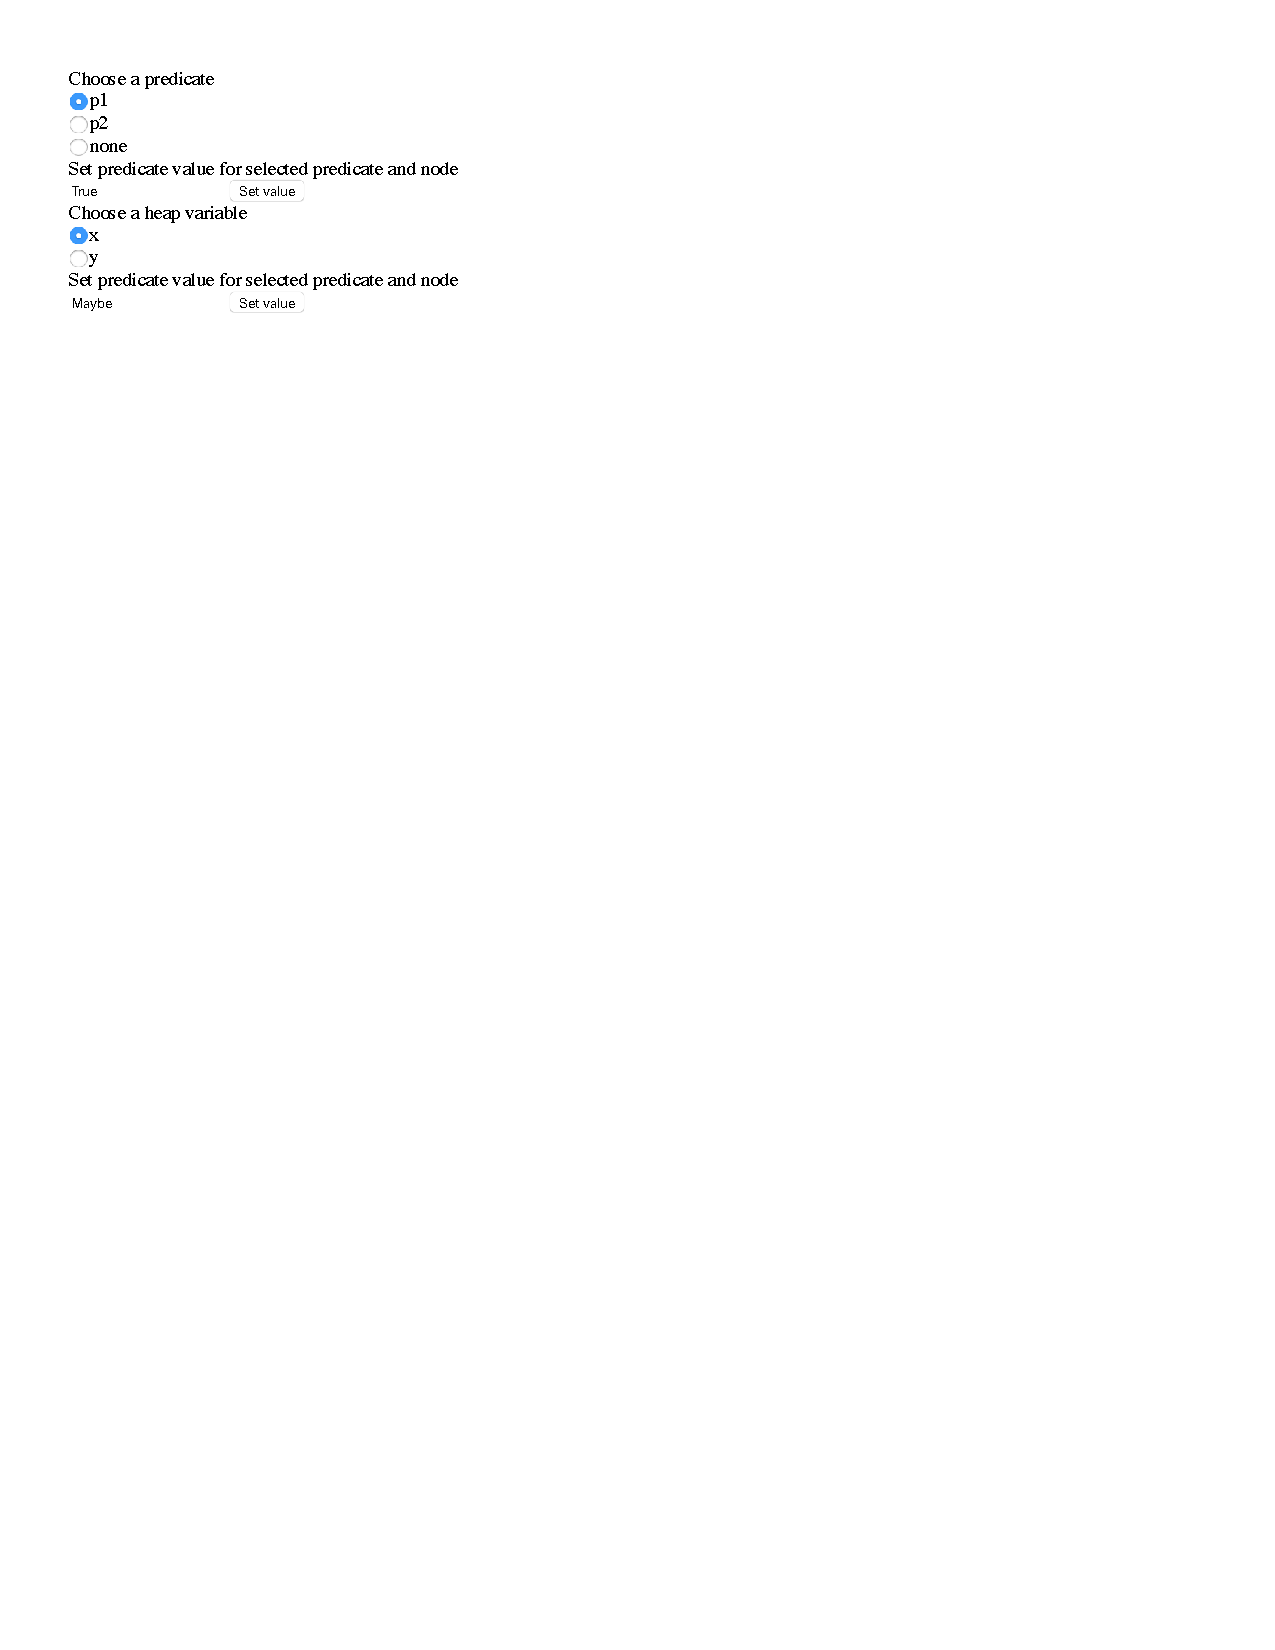
\includegraphics[width=7cm]{fig/predicate-heapvar-val.pdf}
  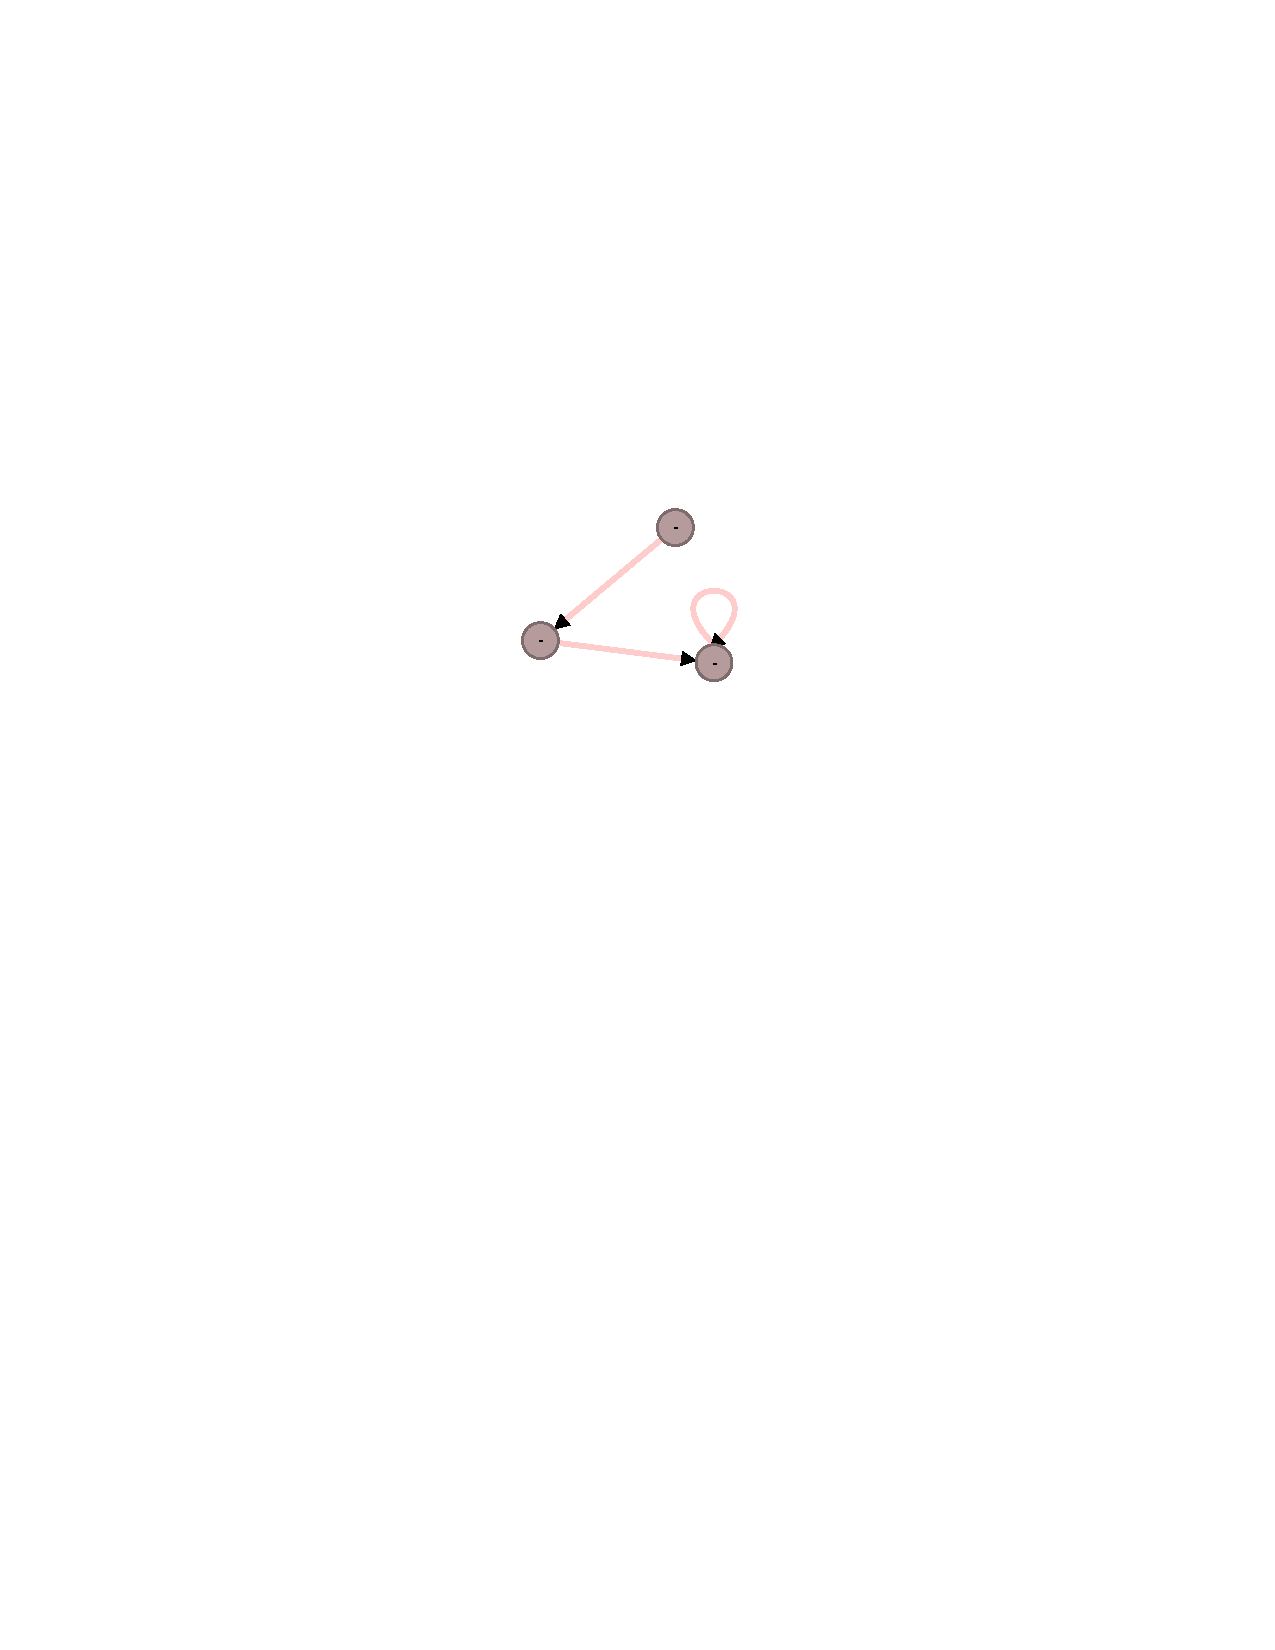
\includegraphics[width=7cm]{fig/basic-graph.pdf}
  \caption{A simple interface to allow the user to graphically draw the heap pattern, and pick values for the predicate and heap variable labeling. The predicates and heap variables have been chosen and populated from a prior analysis. Nodes are represented by circles, and edges as arrows between nodes.
  }
  \label{fig:basic-graph-interface}
\end{figure}

\subsubsection{Who are the Users?}
\label{sec:who-are-the-users}
Our system involves human users, so it is important to describe suitable candidates who will be able to use our system. We believe that a basic understanding of graphs or transition systems should be sufficient, and in fact very helpful in fully grasping what we expect from the user. This means that someone with an undergraduate degree in Computer Science or Mathematics, or indeed anyone who has learned about graphs and state transition systems would be a suitable user. A background in formal methods or verification is not required.

We now dive deeper into all the features provided by the interface, and the user can easily provide a graph pattern matching the formalism described in \autoref{defn:pattern}. One of the important goals of this design is that the user should not have to understand or deal with the formalism itself, but just figures, so that someone with no knowledge of software verification or heap modeling can perform the function of an Oracle.

A heap pattern is a labeled graph represented by the tuple $(\nodesnm, \varlblnm, \predlblnm, \edgesnm, \sigma)$, respectively containing the set of nodes, heap variable labeling, predicate labeling, edges, and summary function. Our interface allows the user to modify the values of each of these attributes of the pattern. We now describe each of these in greater detail.

\subsubsection{Modifying Nodes}
Interacting with nodes allows the user to modify the existing set of nodes. The following actions are available:
\begin{itemize}
  \item Click anywhere on empty space to create a new node.
  \item Click on an existing node to select (or unselect) it. Selected nodes appear a lighter shade than unselected nodes. Only up to one node can be selected at a time.
  \item Press the backspace key after selecting a node to delete it. This deletes all edges and resets other attributes relevant to the node.
\end{itemize}

\autoref{fig:modifying-nodes} illustrates the above points clearly.

% Figure illustrating node modification.
\begin{figure}
  \centering
  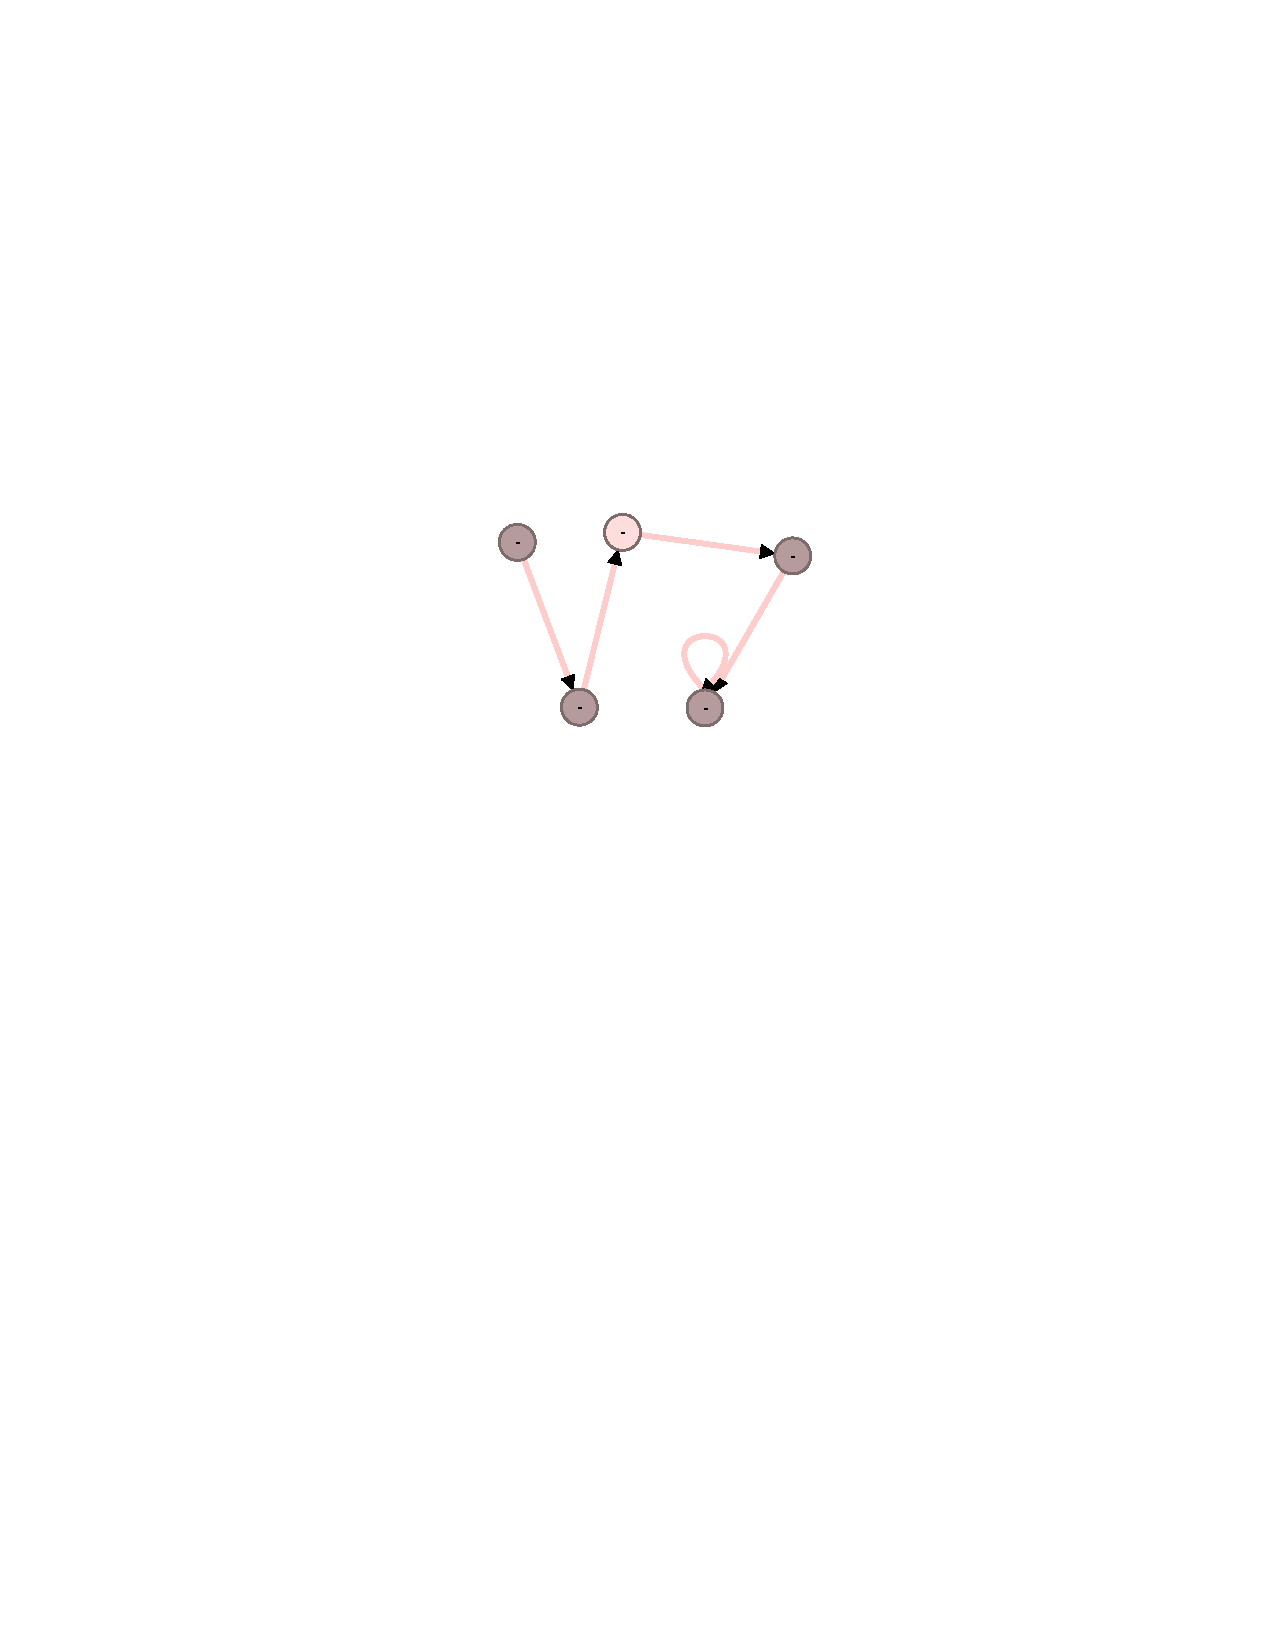
\includegraphics[width=7cm]{fig/nodes-original.pdf}
  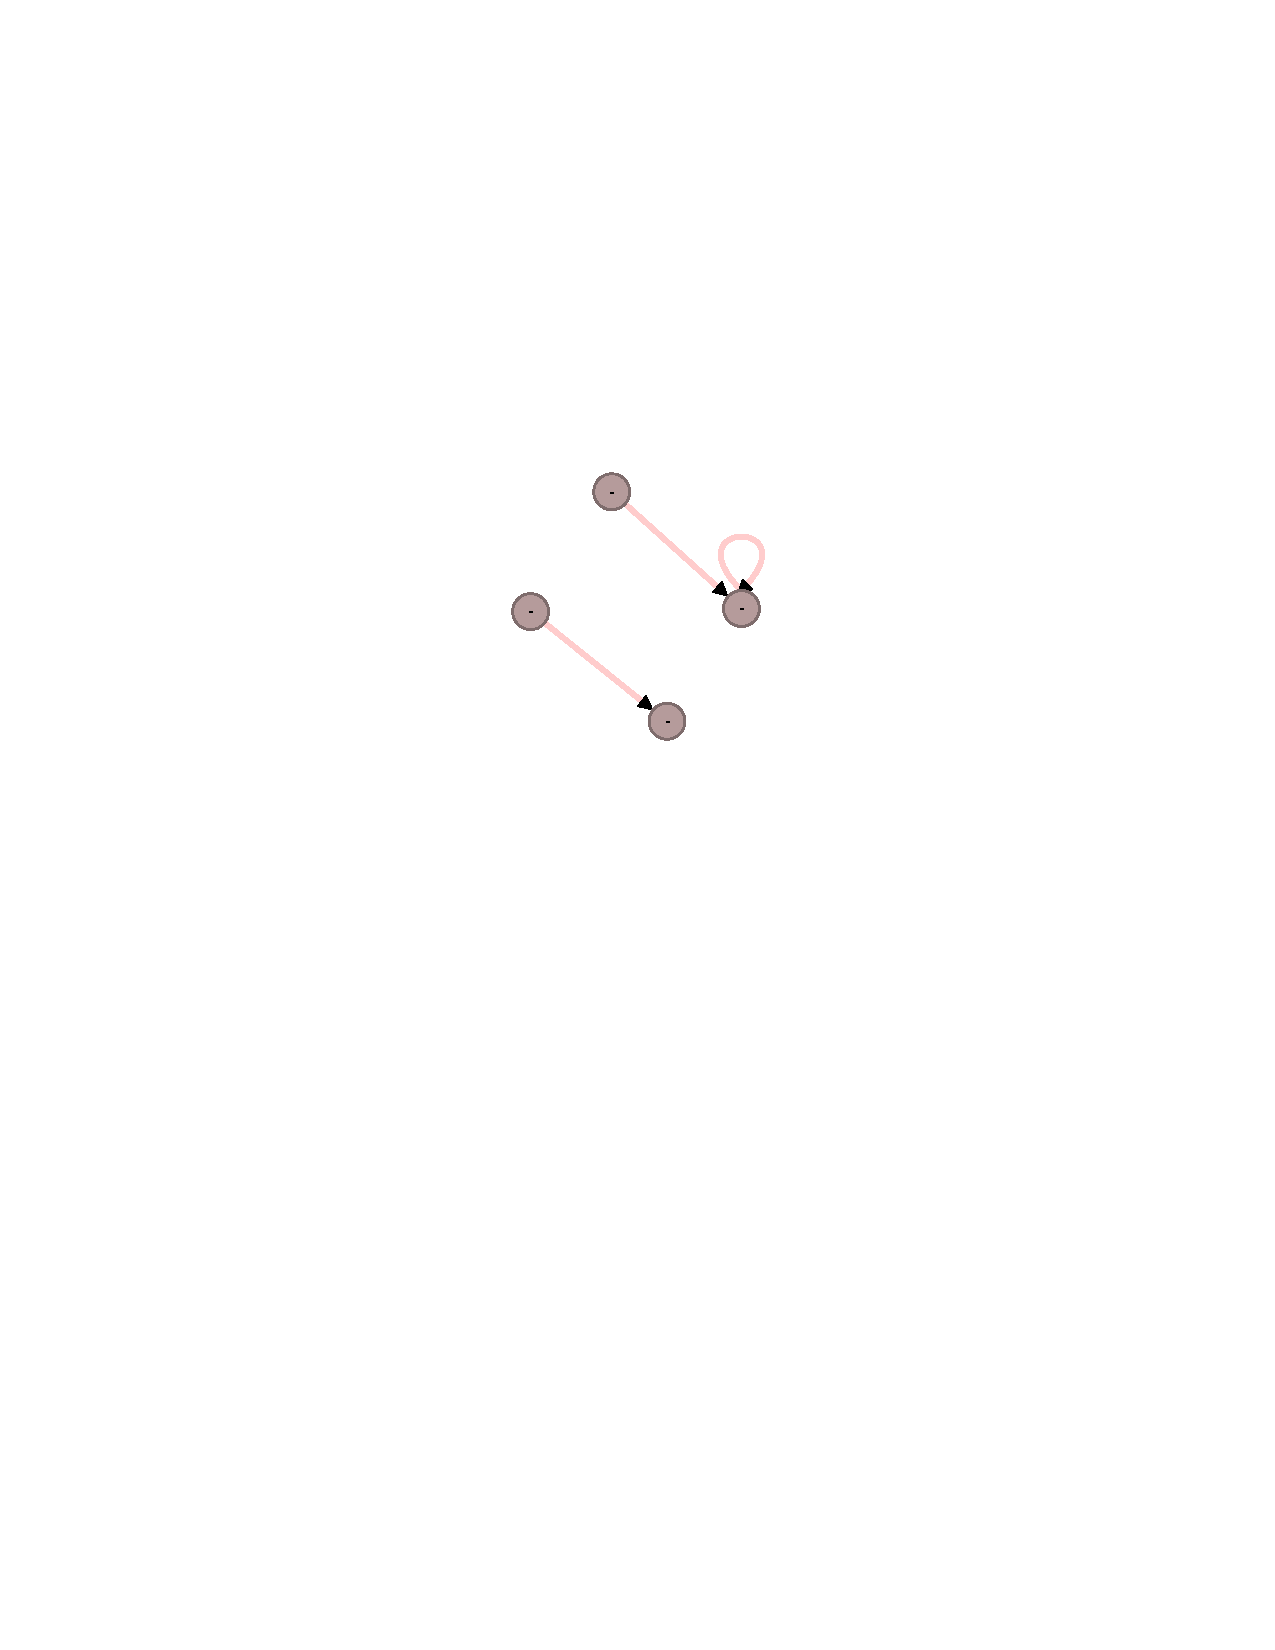
\includegraphics[width=7cm]{fig/nodes-changed.pdf}
  \caption{On the left, the original pattern graph has five nodes, with the middle node selected (indicated by the different color). Pressing the backspace key deletes the node, resulting in the graph on the right.
  }
  \label{fig:modifying-nodes}
\end{figure}

\subsubsection{Modifying the Heap Variable Labeling}
We briefly described the mechanism for updating the heap variable labeling in \autoref{ex:basic-graph-interface}. The interface itself is simple, as shown in \autoref{fig:basic-graph-interface}. In addition, there are some features that make it simpler to keep track of assignments, while preventing user mistakes.

The heap variable labeling is a map $\varlblnm: \nodesnm \times \heapvars \to \threevals$, meaning that each pair of node and heap variable must have a value. To indicate the current assignment, we label the node accordingly. For instance, if the current heap variables are $x, y, z$, and for node $n$, the values of $\varlblnm$ are $\varlblnm(n, x) = \maybe, \varlblnm(n, y) = \true, \varlblnm(n, z) = \false$, then the node will get labeled as $x?y$. The $?$ indicates a $\maybe$ value, the absence of a $?$ indicates $\true$, and absence of the variable altogether indicates $\false$. This keeps the labeling simple, preventing clutter from a large number of $\false$ values, while still making it simple to get a quick idea of the current assignments. Finally, a node with no variable assignments will simply have the label $-$.

We note that $\varlblnm$ is not allowed to have arbitrary assignments. For instance, a variable $x$ cannot be $\true$ for more than one node at the same time. Our interface takes care of such constraints as follows:

\begin{itemize}
  \item Setting a variable to $\true$ for a node sets it to $\false$ for all other nodes automatically.
  \item Setting a variable to $\maybe$ for a node sets it to $\maybe$ for the node where it might currently be $\true$.
\end{itemize}

\autoref{fig:modifying-heap-vars} further illustrates how heap variable labeling works.

% Figure illustrating heap var labeling modification.
\begin{figure}
  \centering
  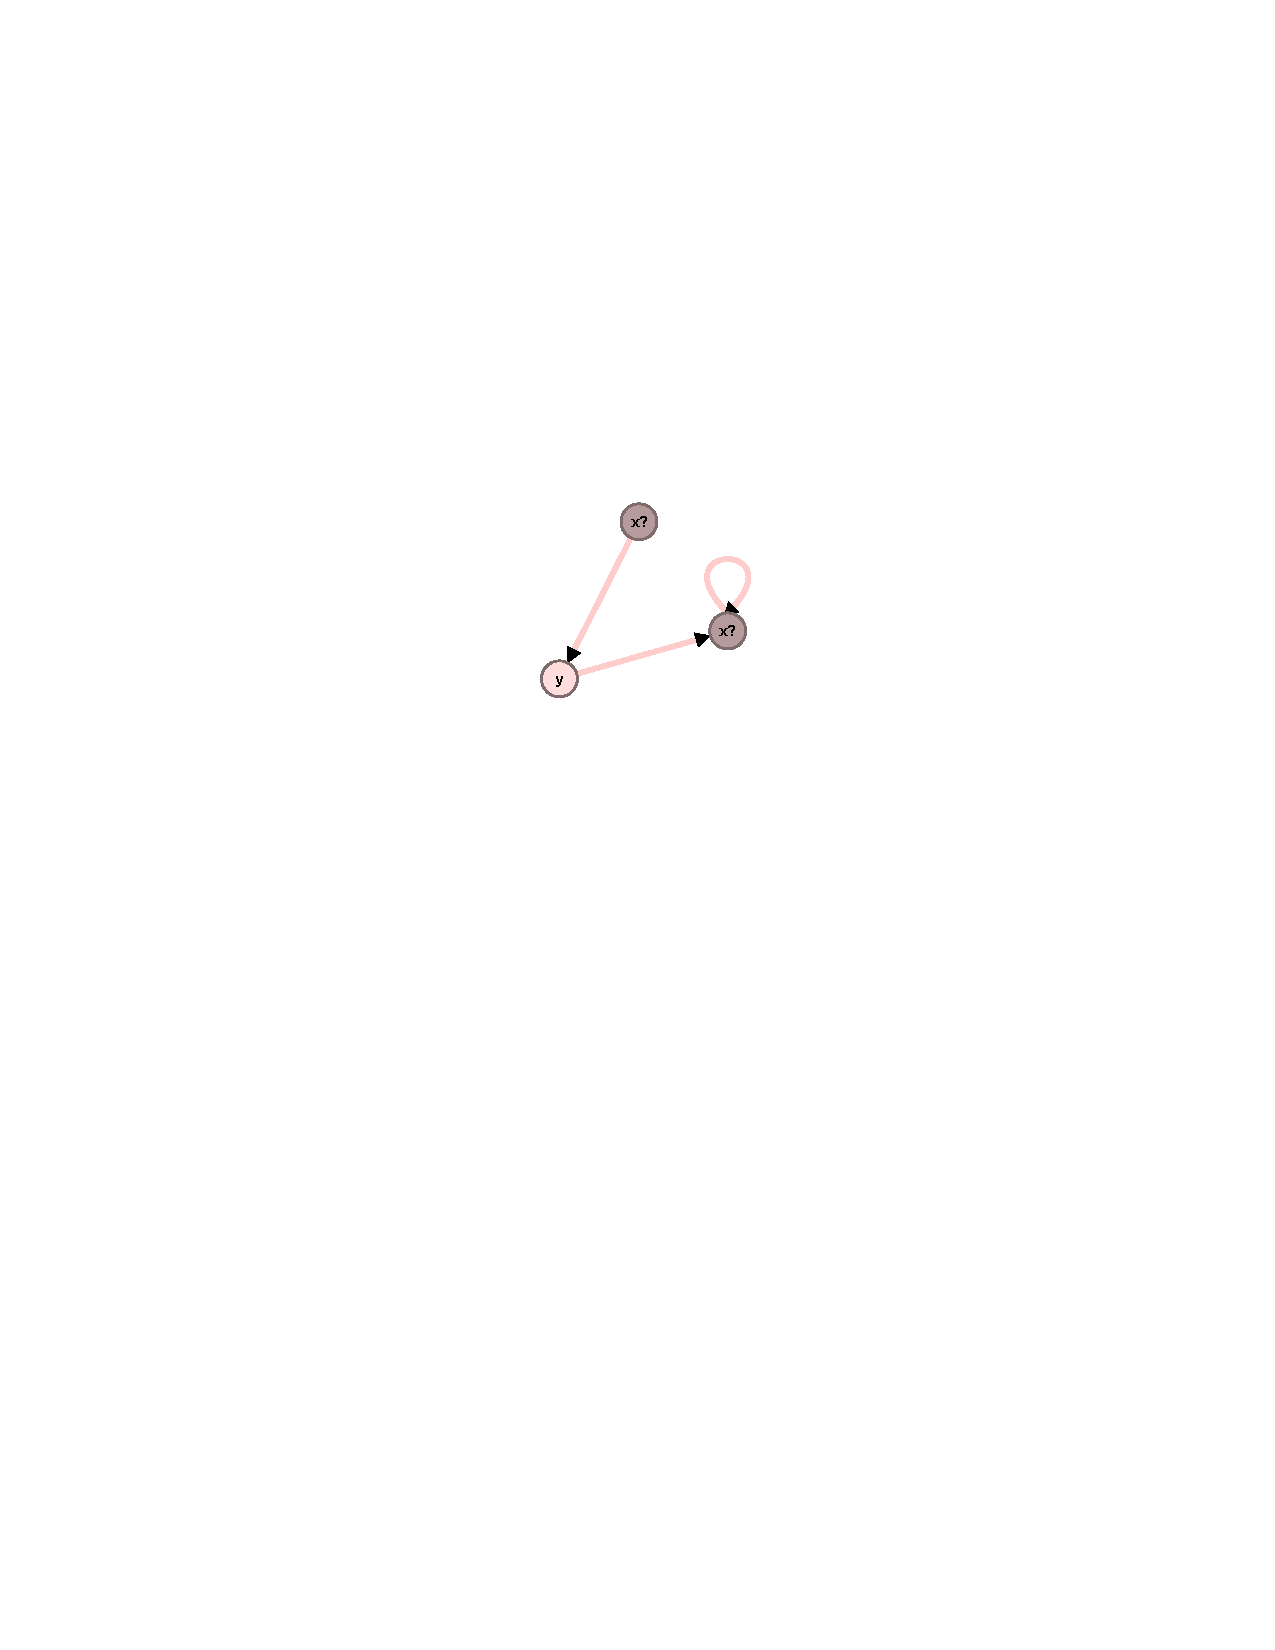
\includegraphics[width=5cm]{fig/heap-var-labeling.pdf}
  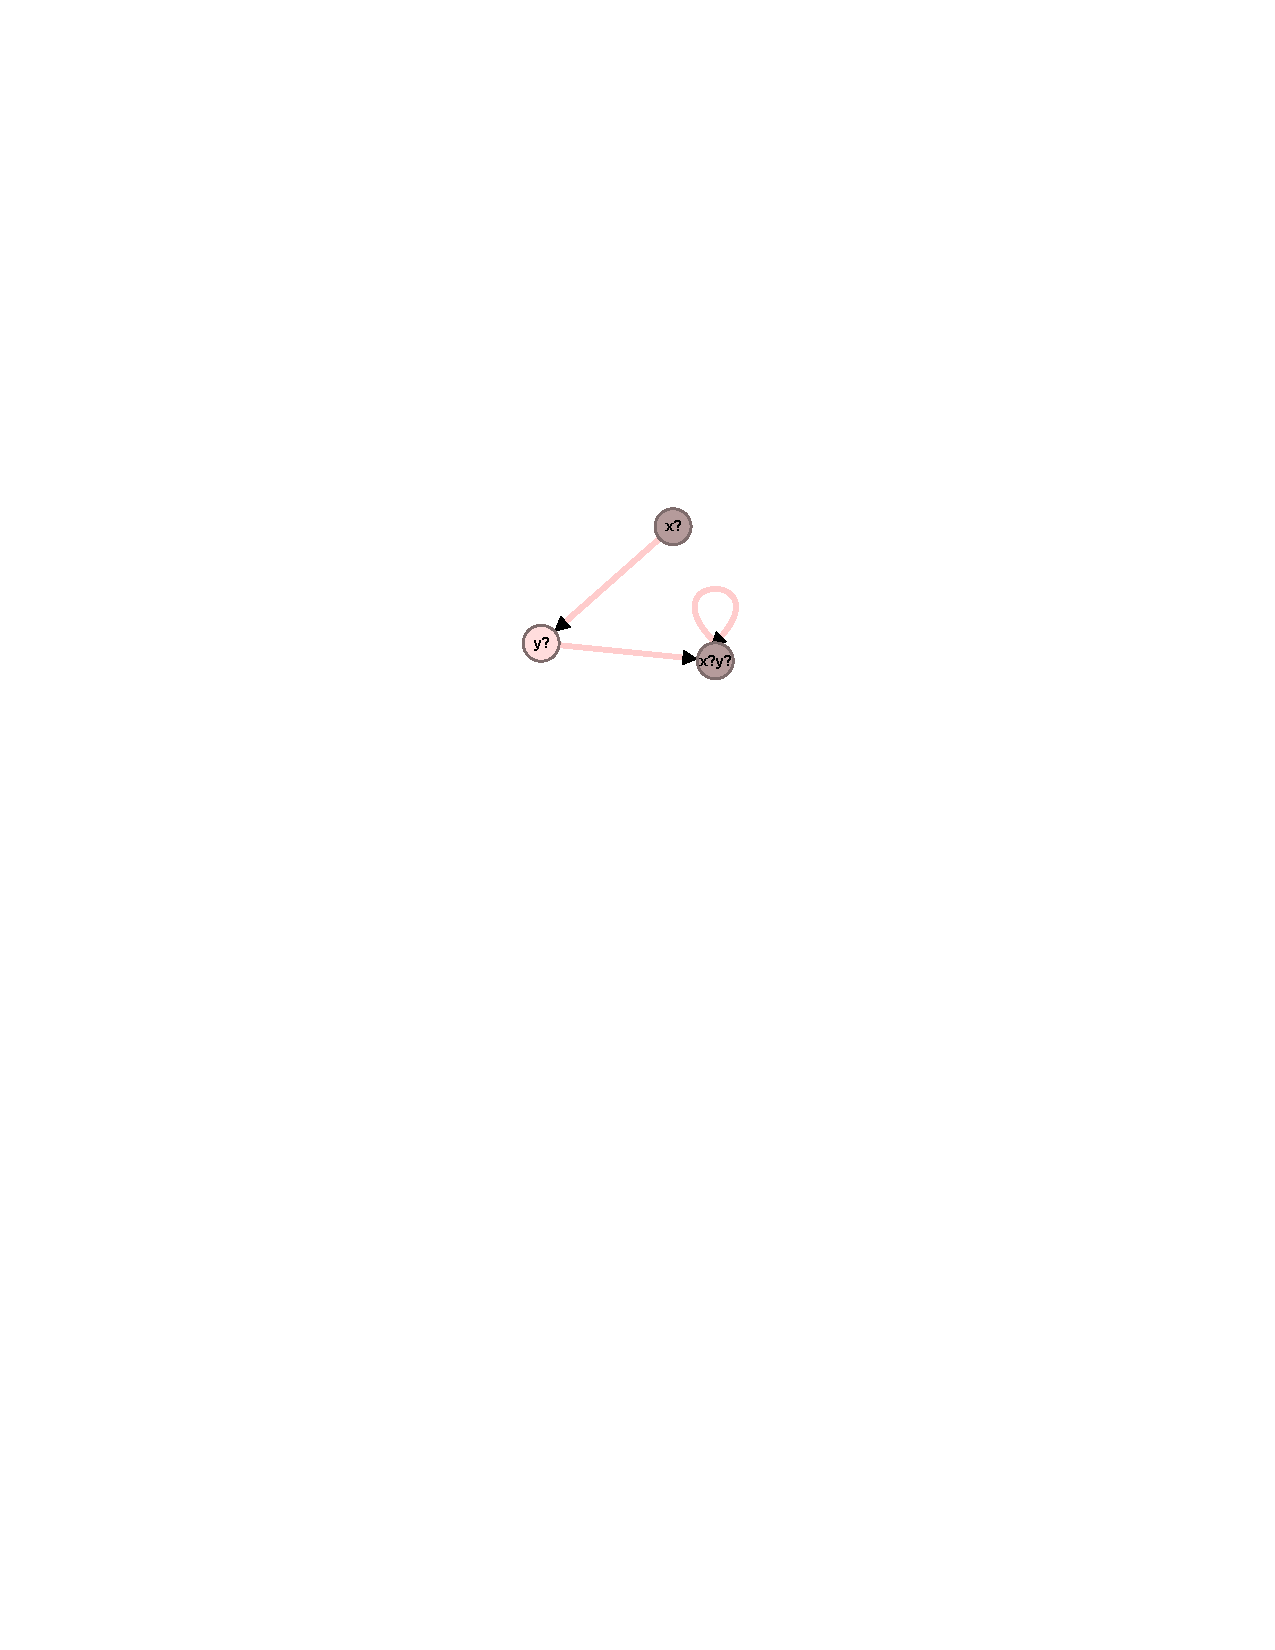
\includegraphics[width=5cm]{fig/heap-var-labeling-2.pdf}
  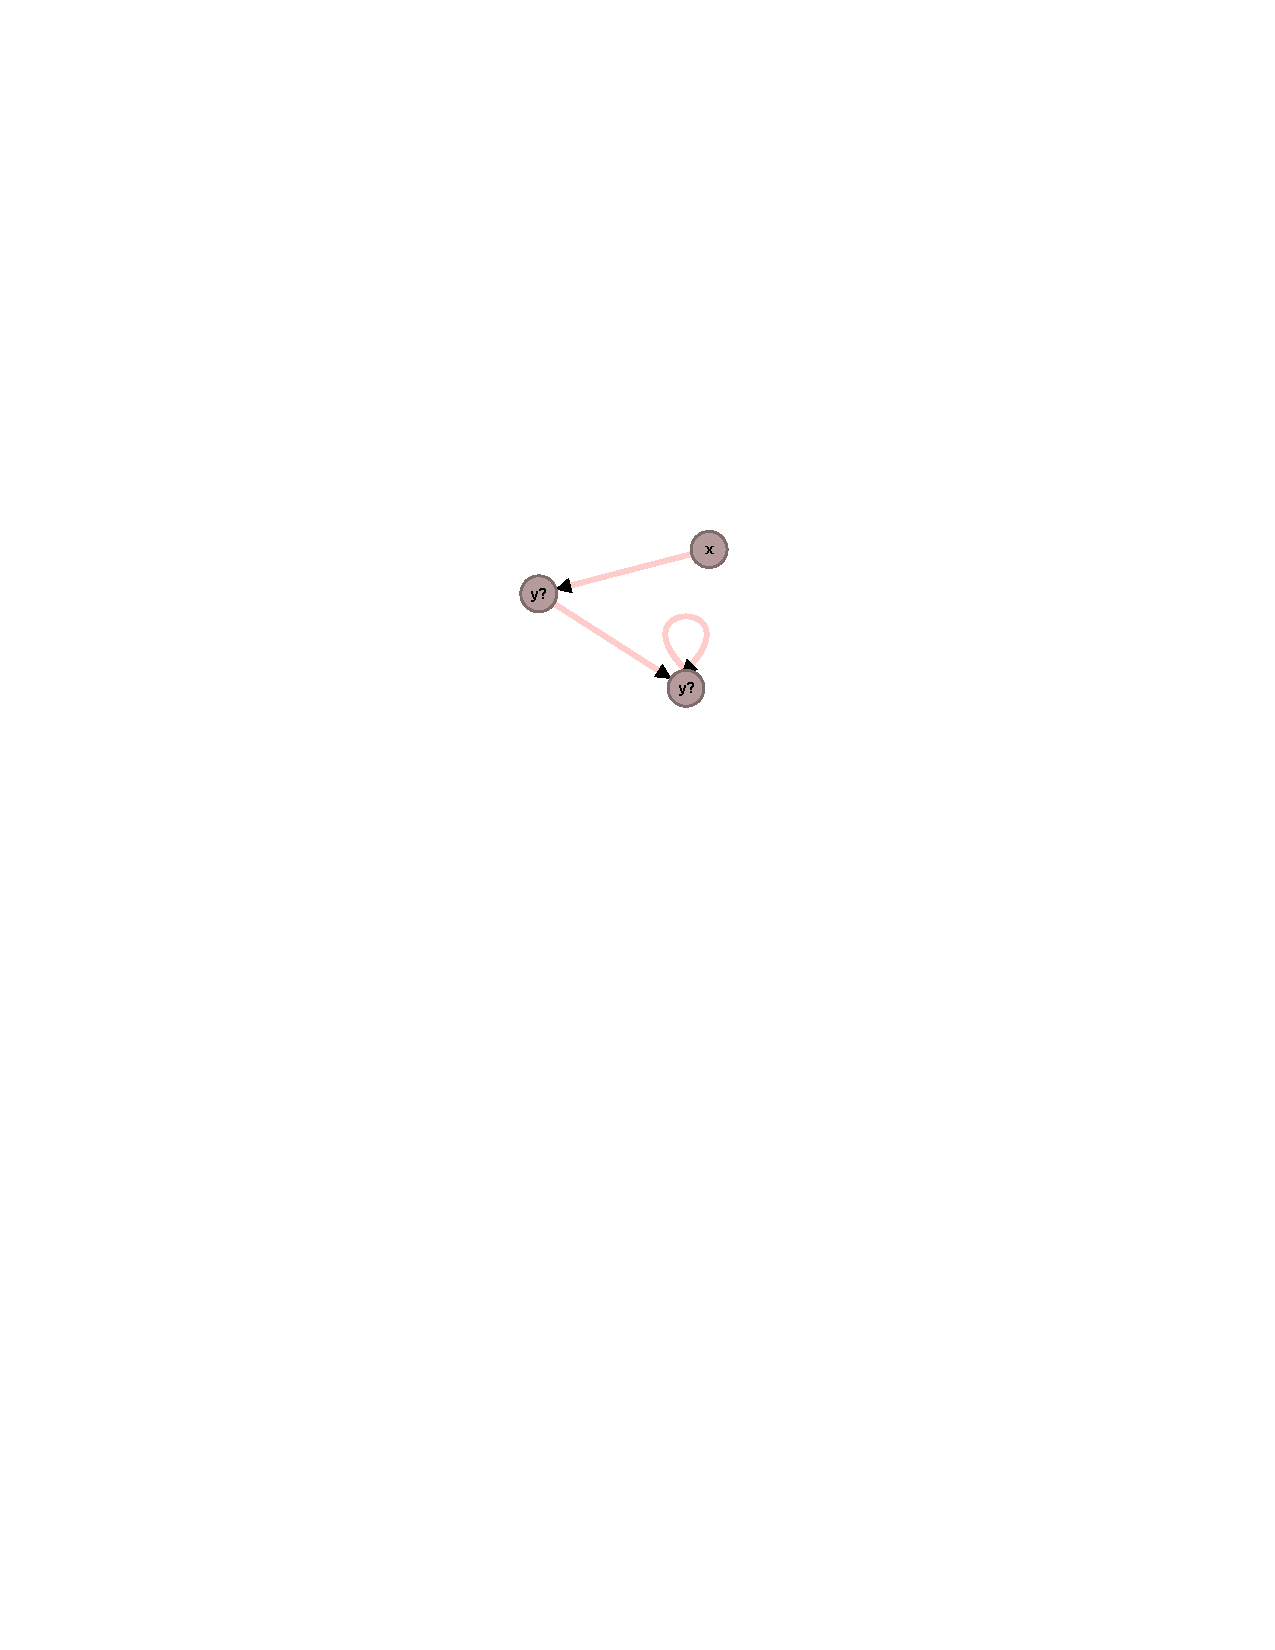
\includegraphics[width=5cm]{fig/heap-var-labeling-3.pdf}
  \caption{The first pattern on the left shows an existing heap variable labeling. We then set the value for $y$ and the node with the self-loop to $\maybe$, which automatically sets the value for $y$ and the selected node to $\maybe$, even though it was $\true$ earlier. Furthermore, in the second pattern, when $x$ is set to $\true$ for the starting node, the value of $x$ is unset for the node with the self-loop.
  }
  \label{fig:modifying-heap-vars}
\end{figure}

\subsubsection{Modifying the Predicate Variable Labeling}
We briefly described the mechanism for updating the predicate variable labeling in \autoref{ex:basic-graph-interface}. The interface itself is simple, as shown in \autoref{fig:basic-graph-interface}. In addition, there are some features that make it simpler to keep track of assignments.

The predicate variable labeling is a map $\predlblnm: \nodesnm \times \predvars \to \threevals$, meaning that each pair of node and predicate variable must have a value. To indicate the current assignment, we use color coding for the nodes - $\predlblnm(n, p) = \true$ imples green, $\predlblnm(n, p) = \false$ imples red, and $\predlblnm(n, p) = \maybe$ implies light pink. Notice that the pattern graph can have multiple predicates available at a time, so the color coding depends on a predicate that is ``live'' at a given time. Predicates can be made live by simply selecting them in the interface shown in \autoref{fig:basic-graph-interface}.

% Figure illustrating pred var modification.
\begin{figure}
  \centering
  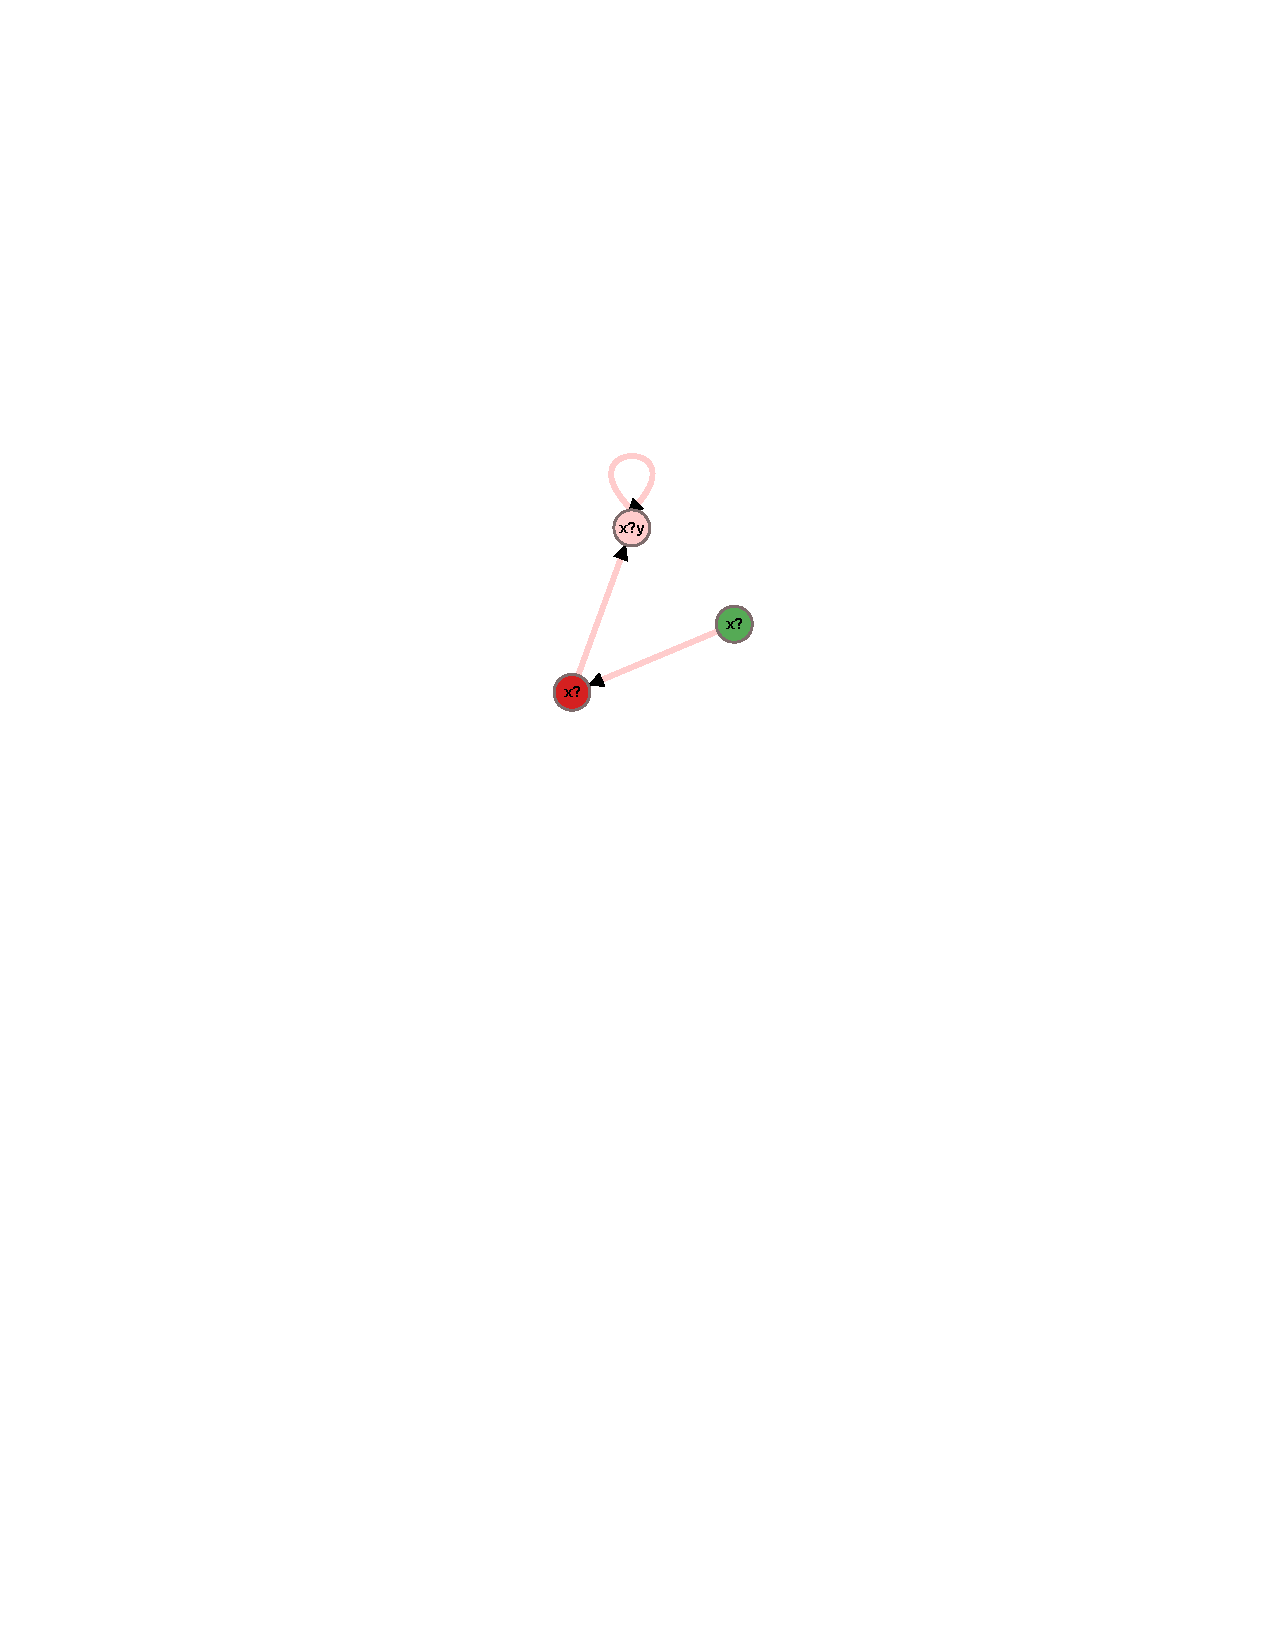
\includegraphics[width=7cm]{fig/predvar.pdf}
  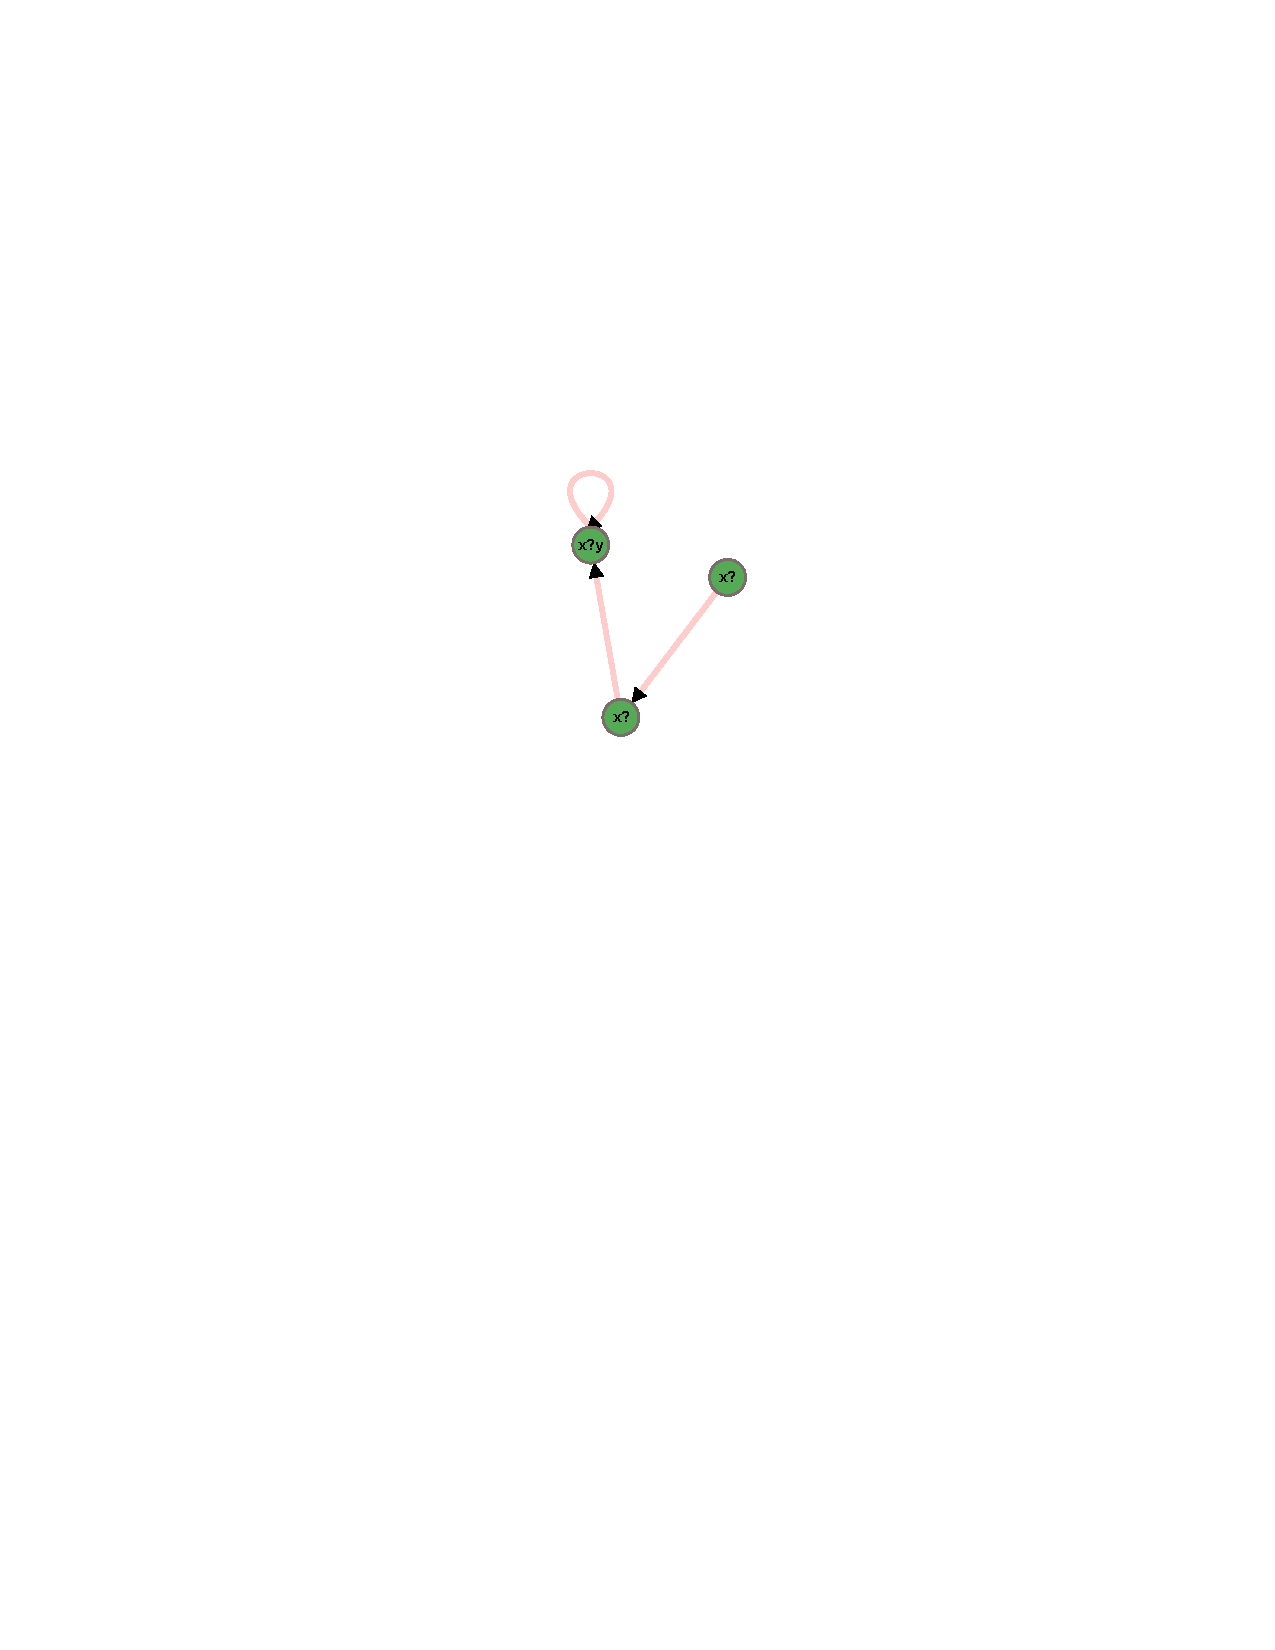
\includegraphics[width=7cm]{fig/predvar2.pdf}
  \caption{On the left, predicate $p1$ is selected, and it has values $\true$, $\false$, and $\maybe$ in order of the arrows, indicated by the appropriate colors. Then we switch the ``live'' predicate to $p2$, which happens to be $\true$ for all nodes, so the color switches to green for each node.}
  \label{fig:modifying-pred-vars}
\end{figure}

\autoref{fig:modifying-pred-vars} illustrates how predicate variable labeling looks.

\subsubsection{Modifying Edges}
Edges are represented by the map $\edgesnm: \nodesnm \times \fields \times \nodesnm \to \threevals$. For our case, since we're only dealing with a single field in the interface, the map can be simplified to $\edgesnm: \nodesnm \times \nodesnm \to \threevals$, meaning that each pair of nodes have an edge between them in either direction. For two nodes $m, n$, $\edgesnm(m, n) = \true$ implies that a green edge exists pointing from $m$ to $n$. $\edgesnm(m, n) = \maybe$ implies that the edge is light pink instead. If $\edgesnm(m, n) = \false$, then this is indicated by the absence of an edge. Once again, this is to make sure that the pattern graph isn't overly cluttered because of too many $\false$ edges. An edge is also a link for the force-directed graph in D3.

Interacting with edges is fairly simple:
\begin{itemize}
  \item Drag the mouse from a node to another to create an edge between them, in the direction of dragging.
  \item Click on an existing edge to select (or unselect) it. Selected edges appear dotted, as opposed to solid for unselected edges. Only up to one edge can be selected at a time.
  \item Press the backspace key after selecting a edge to delete it.
  \item Pressing the M key for a selected edge toggles between $\true$ and $\maybe$ values for that edge (respectively green and light pink).
  \item Pressing the R key for a selected node creates a self-loop on that node. Each node can have only one self-loop, and all edge interactions work for it just like other edges.
\end{itemize}

% Figure illustrating edge modification.
\begin{figure}
  \centering
  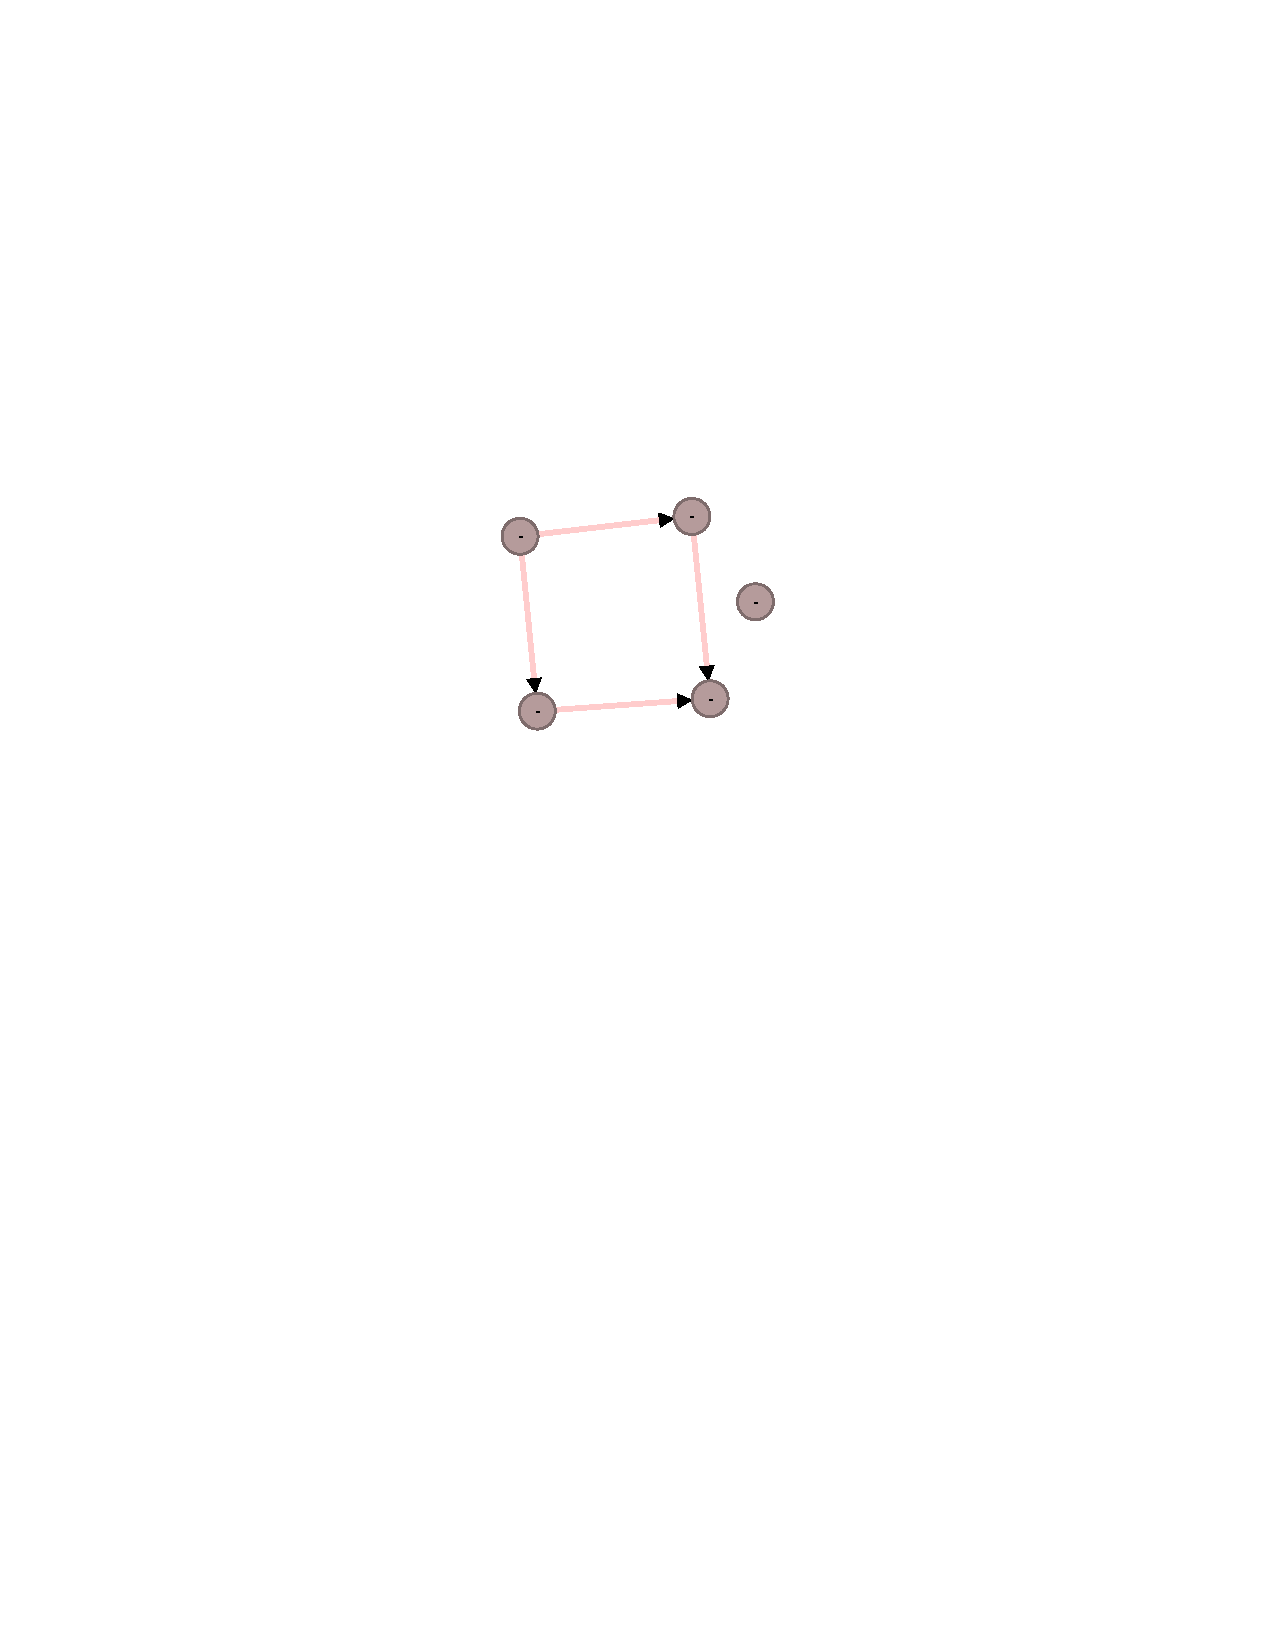
\includegraphics[width=5cm]{fig/edges1.pdf}
  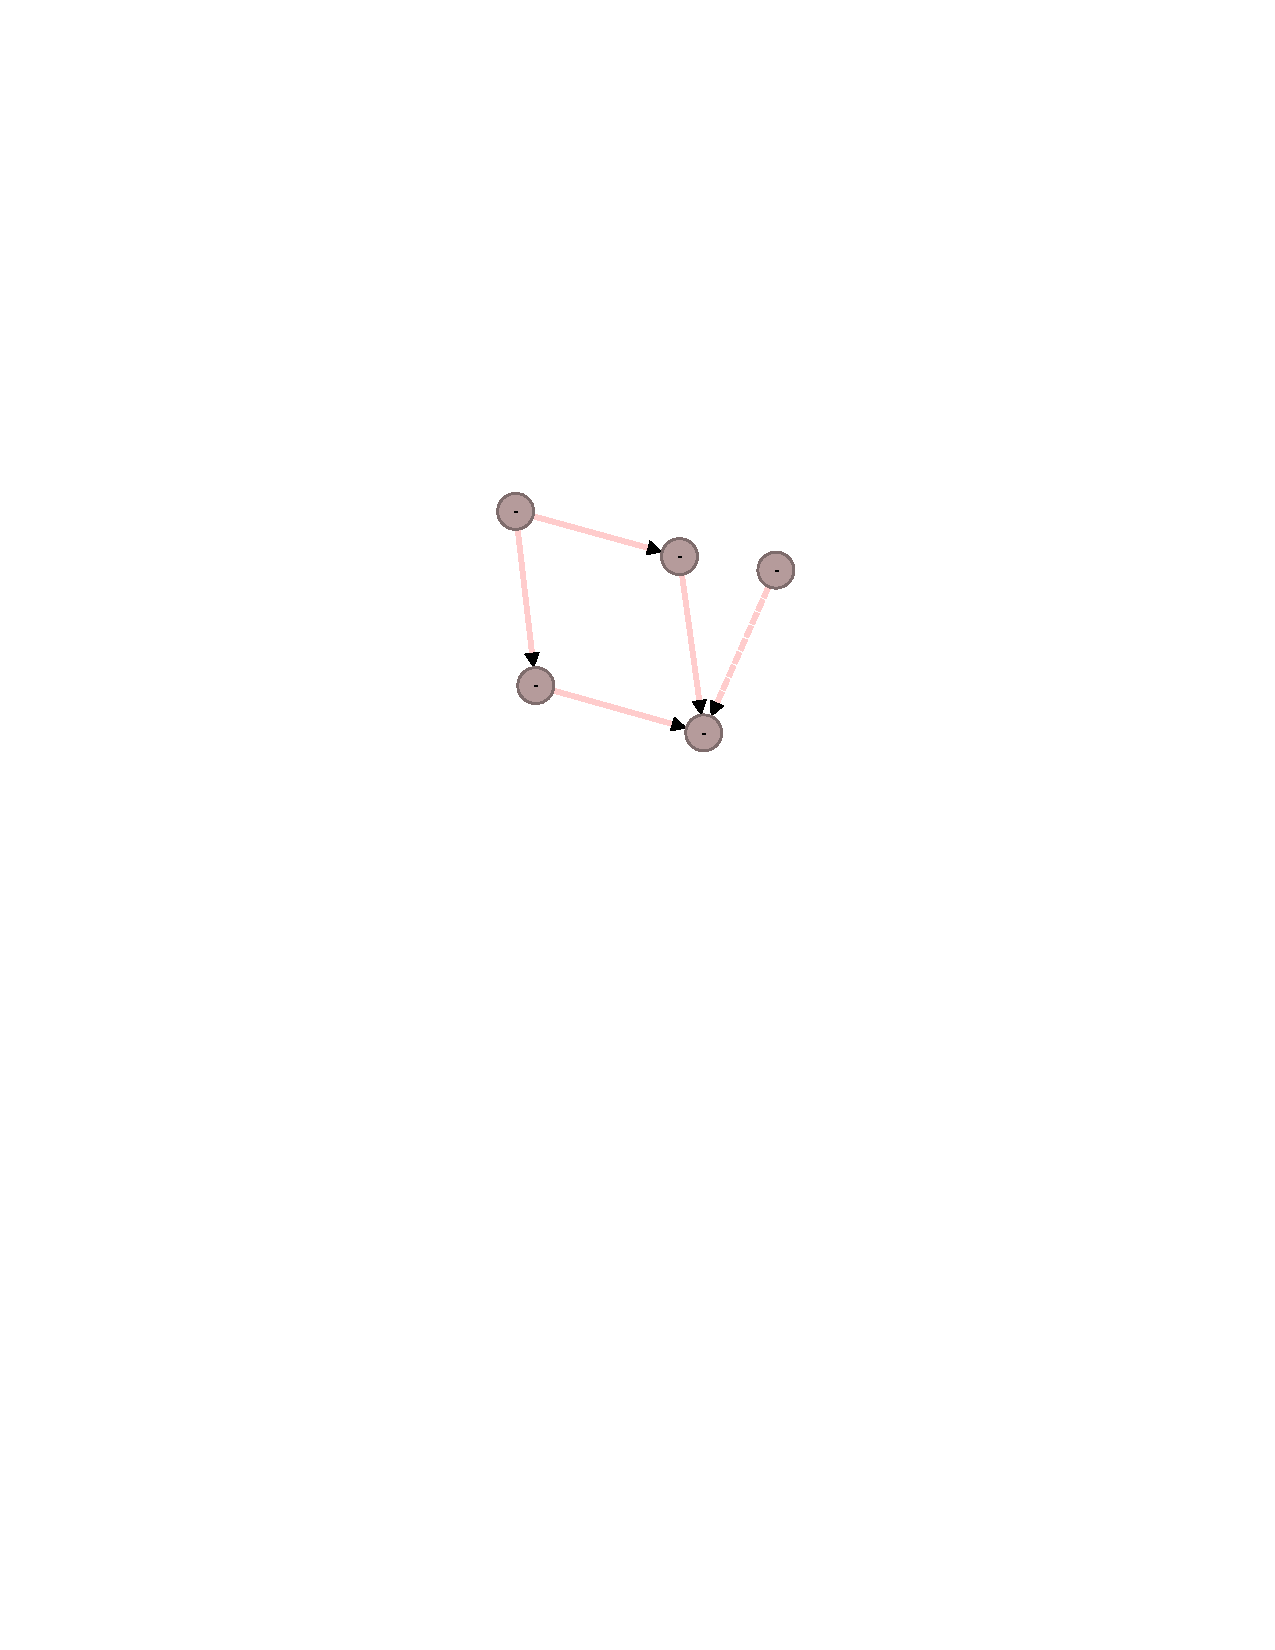
\includegraphics[width=5cm]{fig/edges2.pdf}
  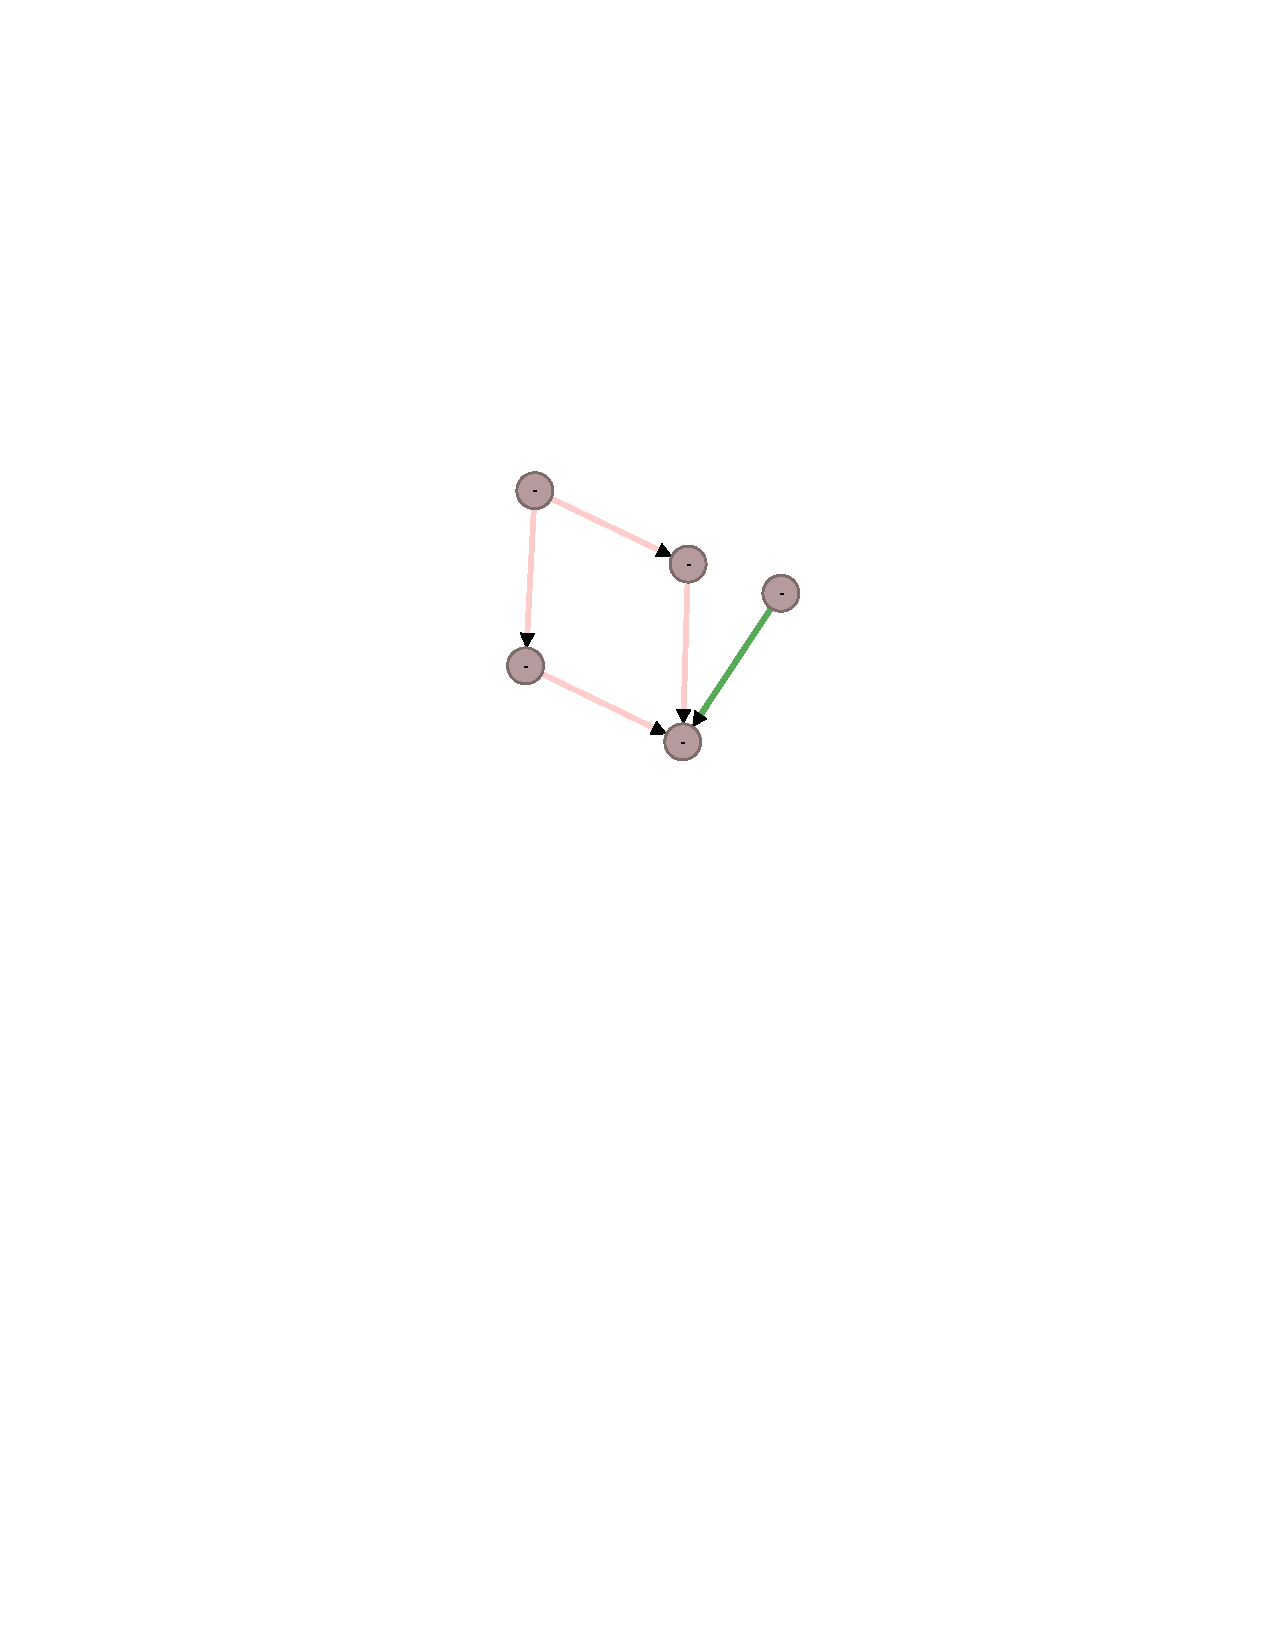
\includegraphics[width=5cm]{fig/edges3.pdf}
  \caption{The first pattern on the left has a node $n$ that is not connected to any other node. We drag from $n$ to another node to create a new edge, which is also selected in the second pattern (indicated by the dotted line). For the selected edge, we press the M key, which turns it into a $\true$ (green) edge, in the third pattern on the right.}
  \label{fig:modifying-edges}
\end{figure}

Edges are normally straight, but bidirectional edges are rounded for better visibility. \autoref{fig:modifying-edges} illustrates how the interface allows for interaction with edges.

Just like $\varlblnm$, $\edgesnm$ is not allowed to have arbitrary assignments. For instance, a $\true$ edge going out from a node implies that there cannot be any other edge going out of the same node. Our interface takes care of such constraints as follows:

\begin{itemize}
  \item Setting an edge (from node $m$ to $n$) to $\true$ sets all outgoing edges from $m$ $\false$ automatically i.e. deletes them.
  \item Setting an edge (from node $m$ to $n$) to $\maybe$ sets any $\true$ outgoing edge from $m$ to $\maybe$ automatically.
\end{itemize}

% Figure illustrating enforcement of edge constraints.
\begin{figure}
  \centering
  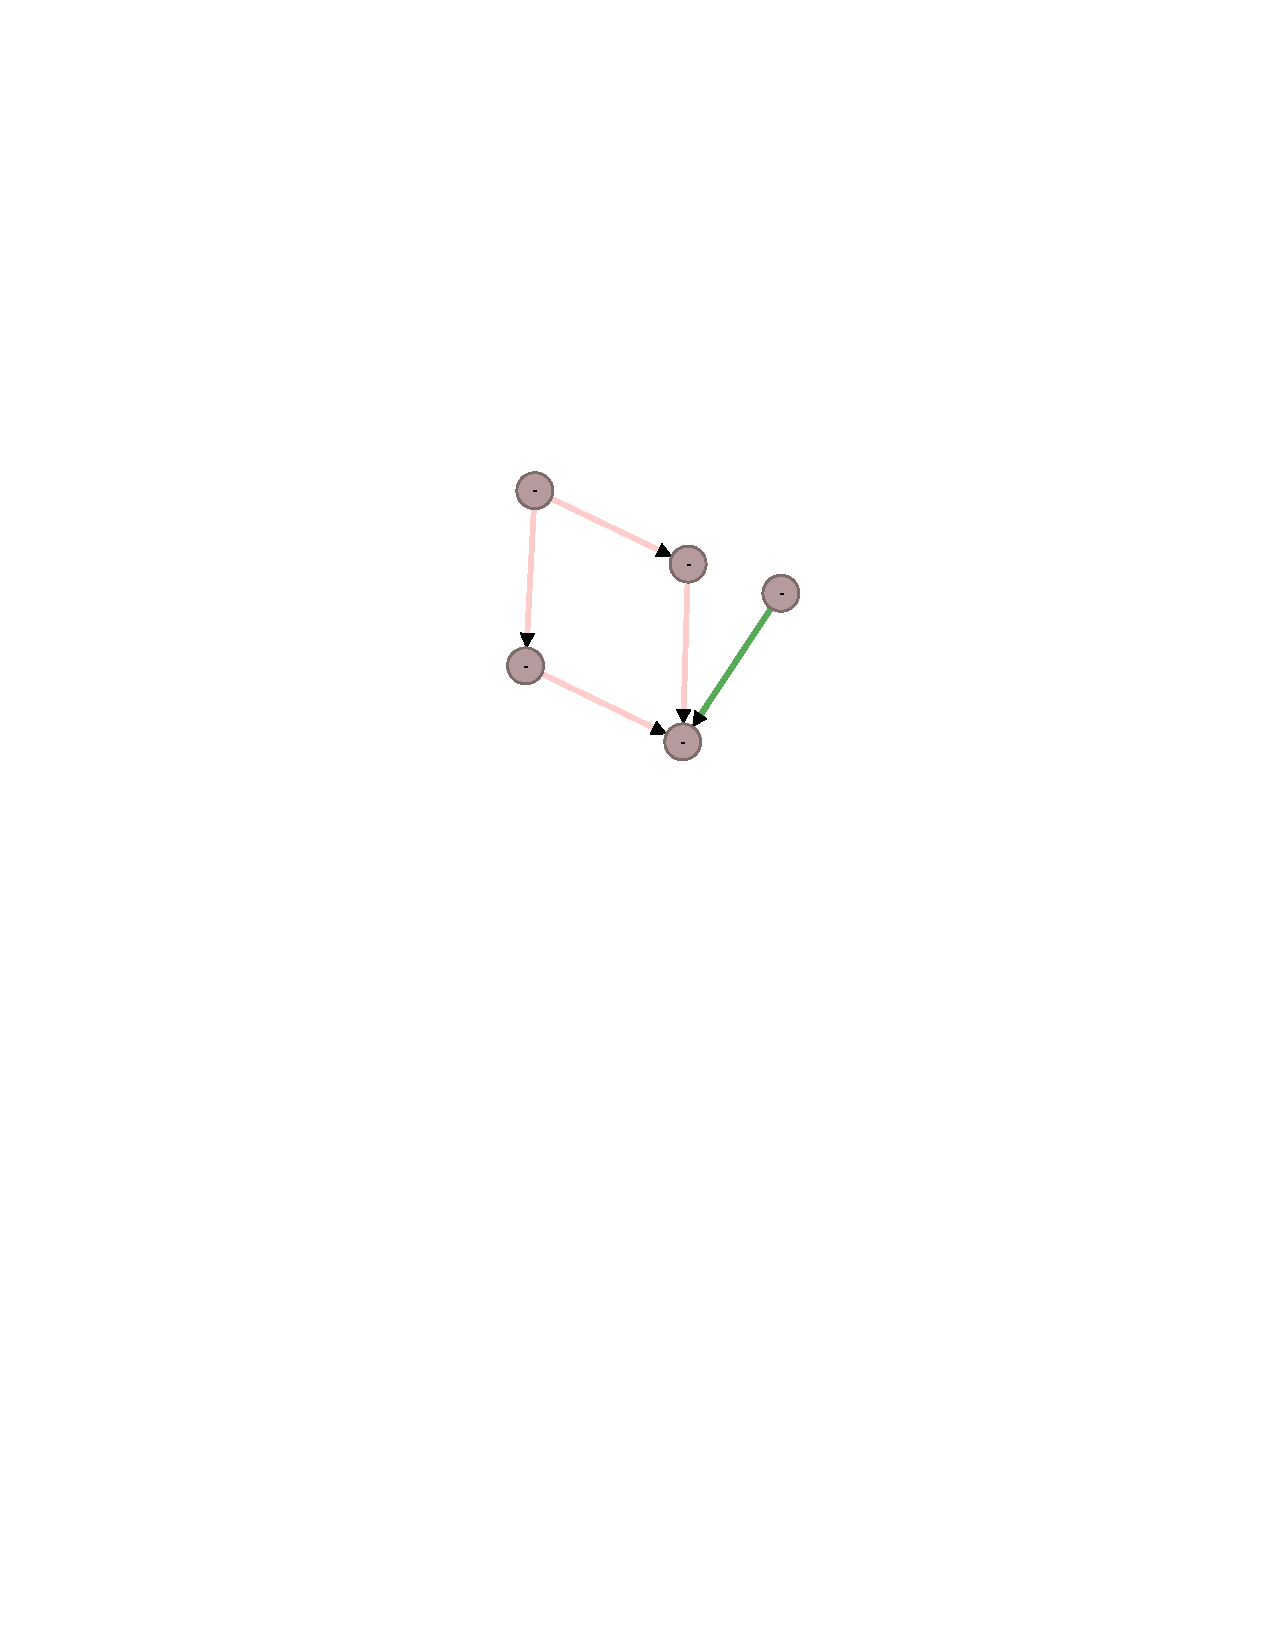
\includegraphics[width=5cm]{fig/edges3.pdf}
  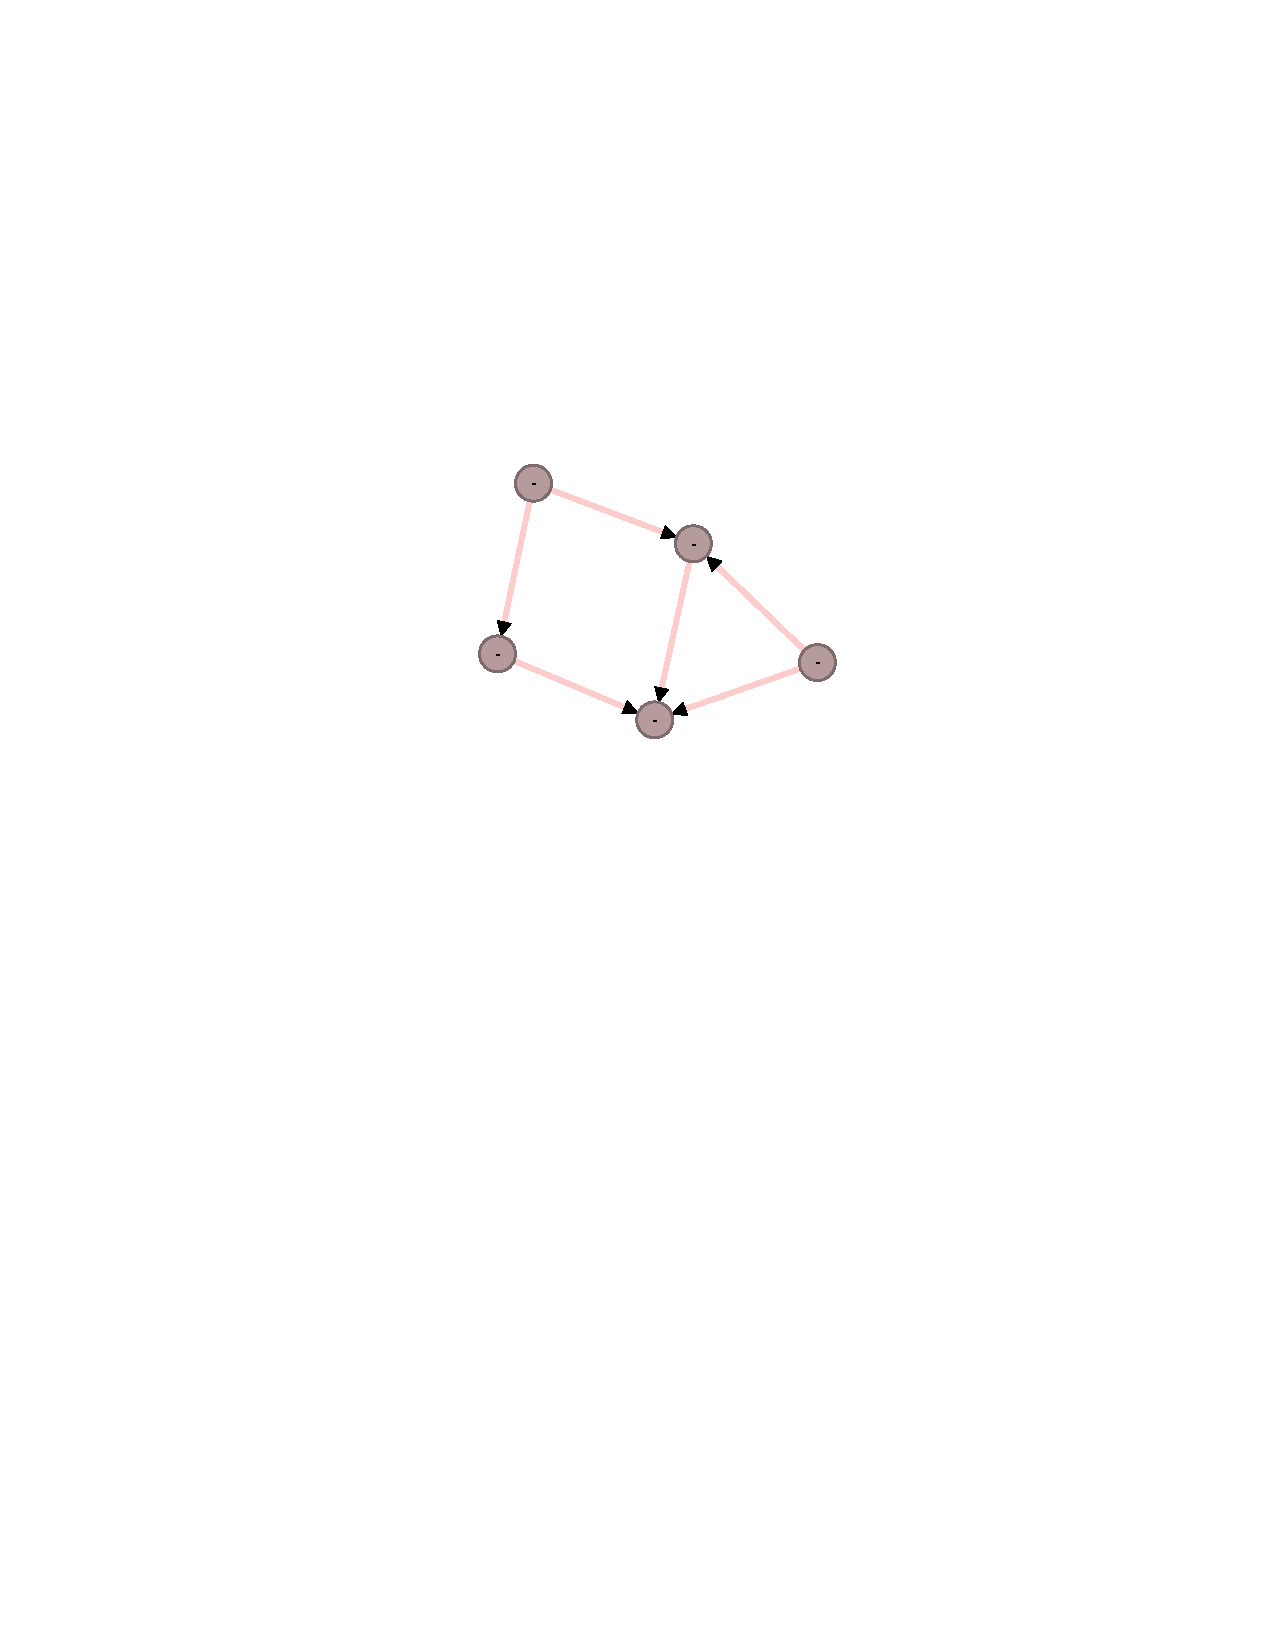
\includegraphics[width=5cm]{fig/edge-constraints-1.pdf}
  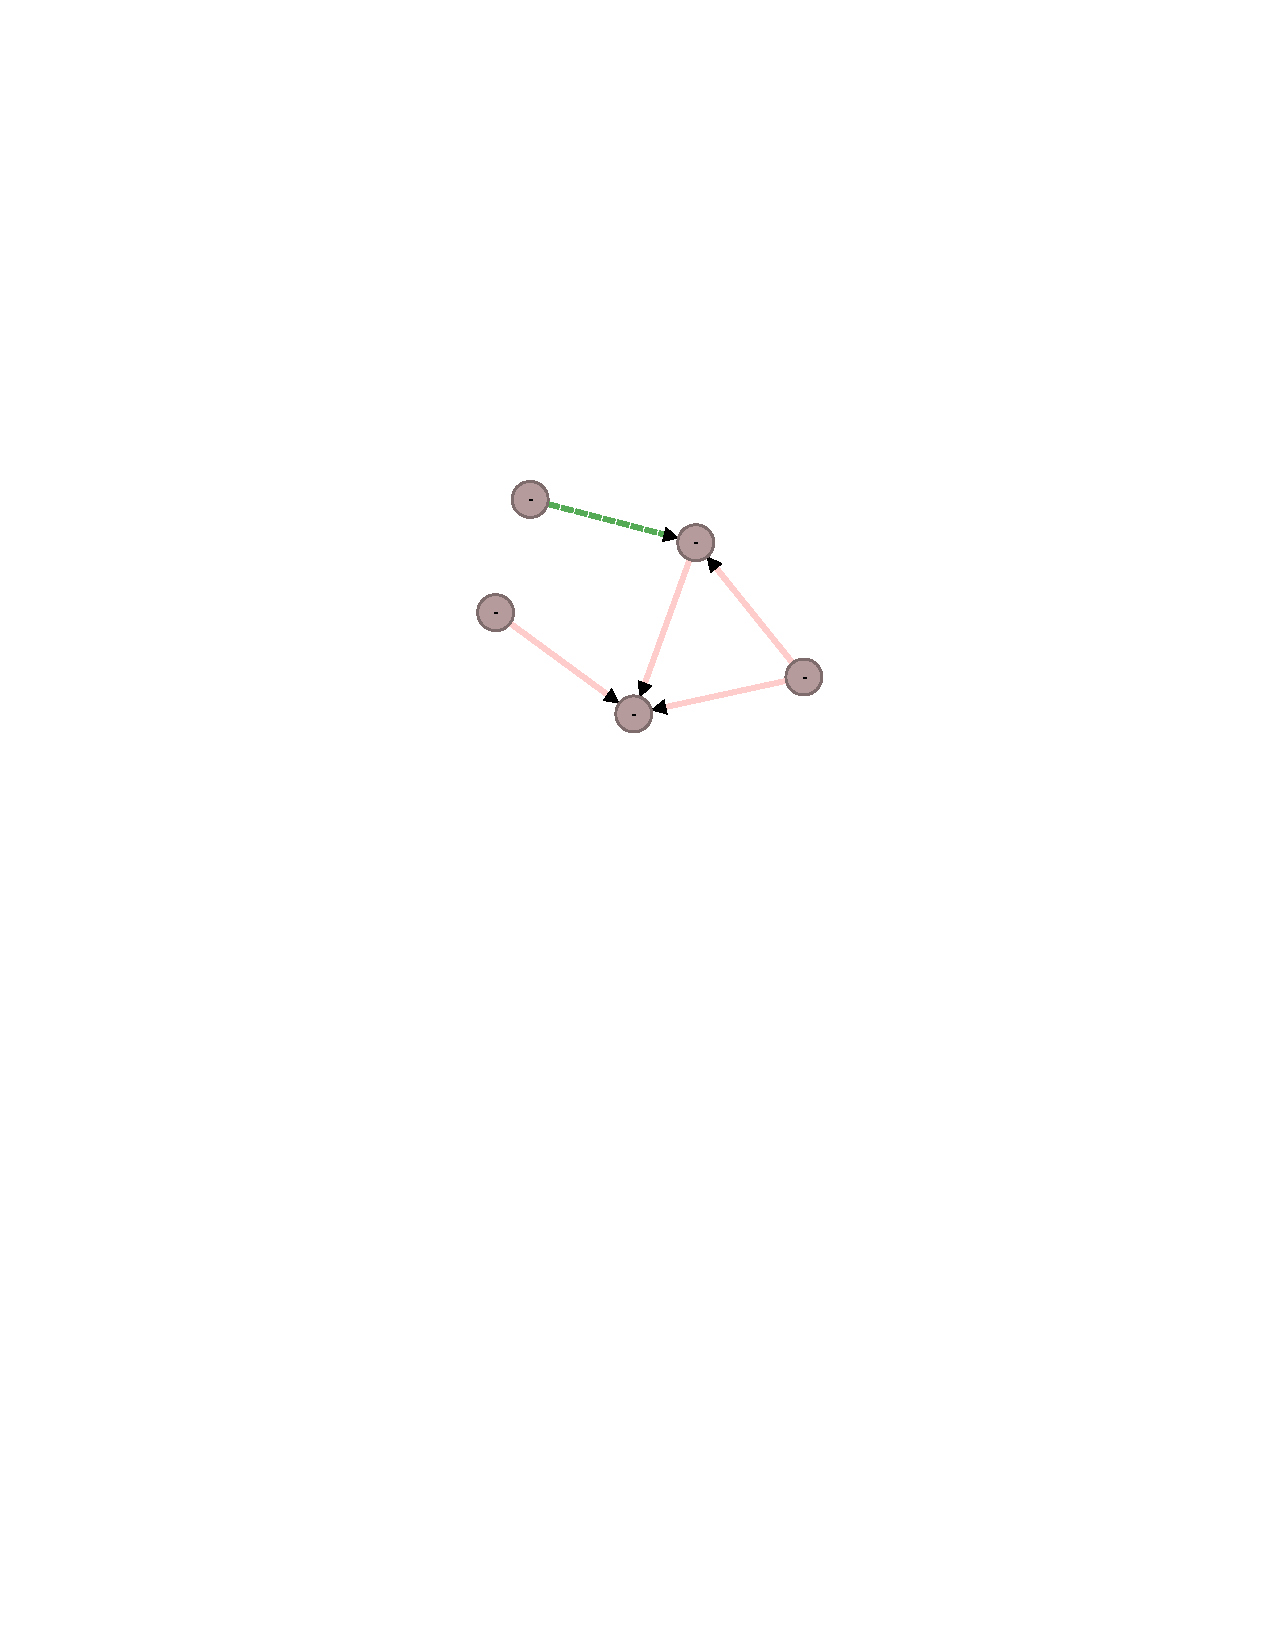
\includegraphics[width=5cm]{fig/edge-constraints-2.pdf}
  \caption{The first figure on the left has a node $n$ with a $\true$ outgoing edge. We create another outgoing edge from $n$, which is a $\maybe$ edge by default, but it also turns the $\true$ edge to $\maybe$. In the third pattern on the right, we turn a $\maybe$ edge to $\true$, which results in the other $\maybe$ edge going out of it disappearing (becoming $\false$).}
  \label{fig:edge-constraints}
\end{figure}

\autoref{fig:edge-constraints} illustrates how constraints on $\edgesnm$ are enforced by the interface.

\subsubsection{Modifying the Summary Function}
The summary function $\sigma: \nodesnm \to \bools$ indicates where a node is a summary node. Our interface indicates summary nodes by making them larger than other nodes. Selecting a node and pressing the S key toggles the value of $\sigma$ for that node. \autoref{fig:summary-nodes} illustrates an example of this.

% Figure illustrating pred var modification.
\begin{figure}
  \centering
  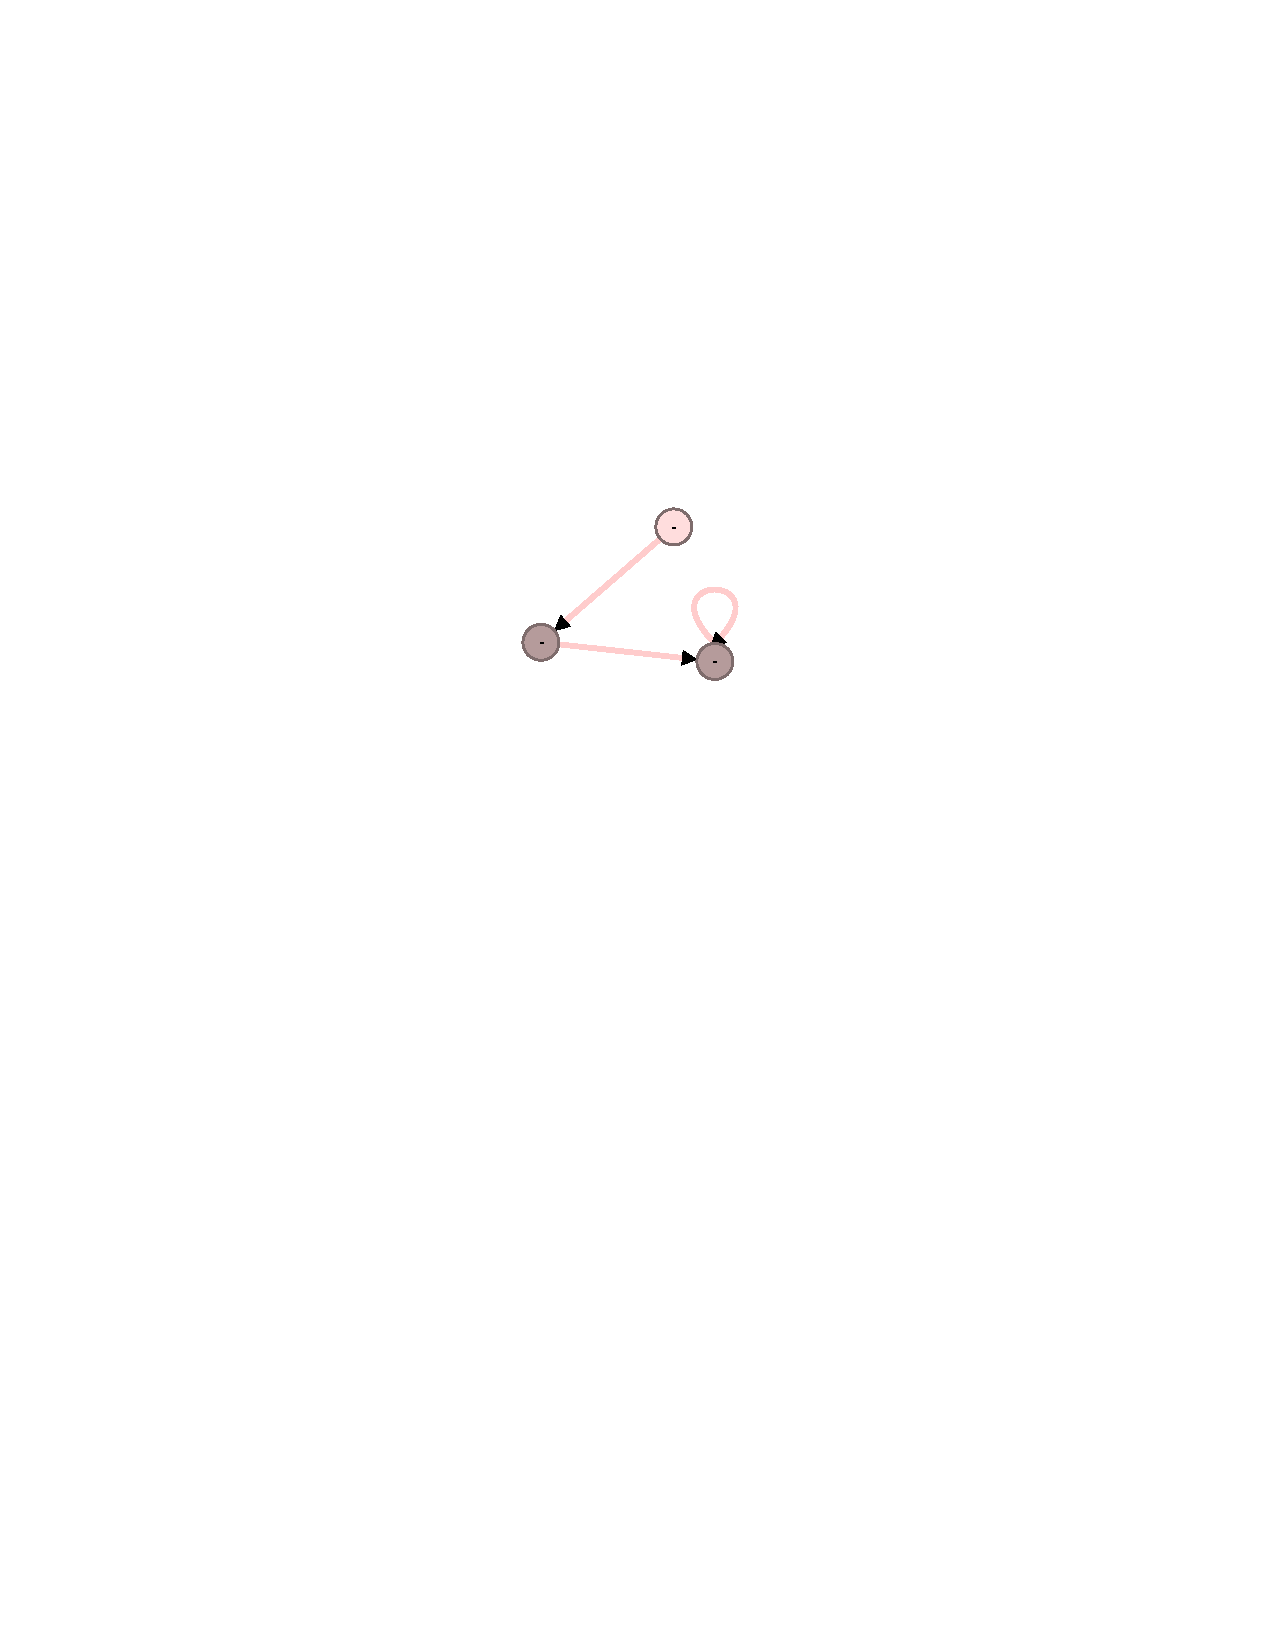
\includegraphics[width=7cm]{fig/summary1.pdf}
  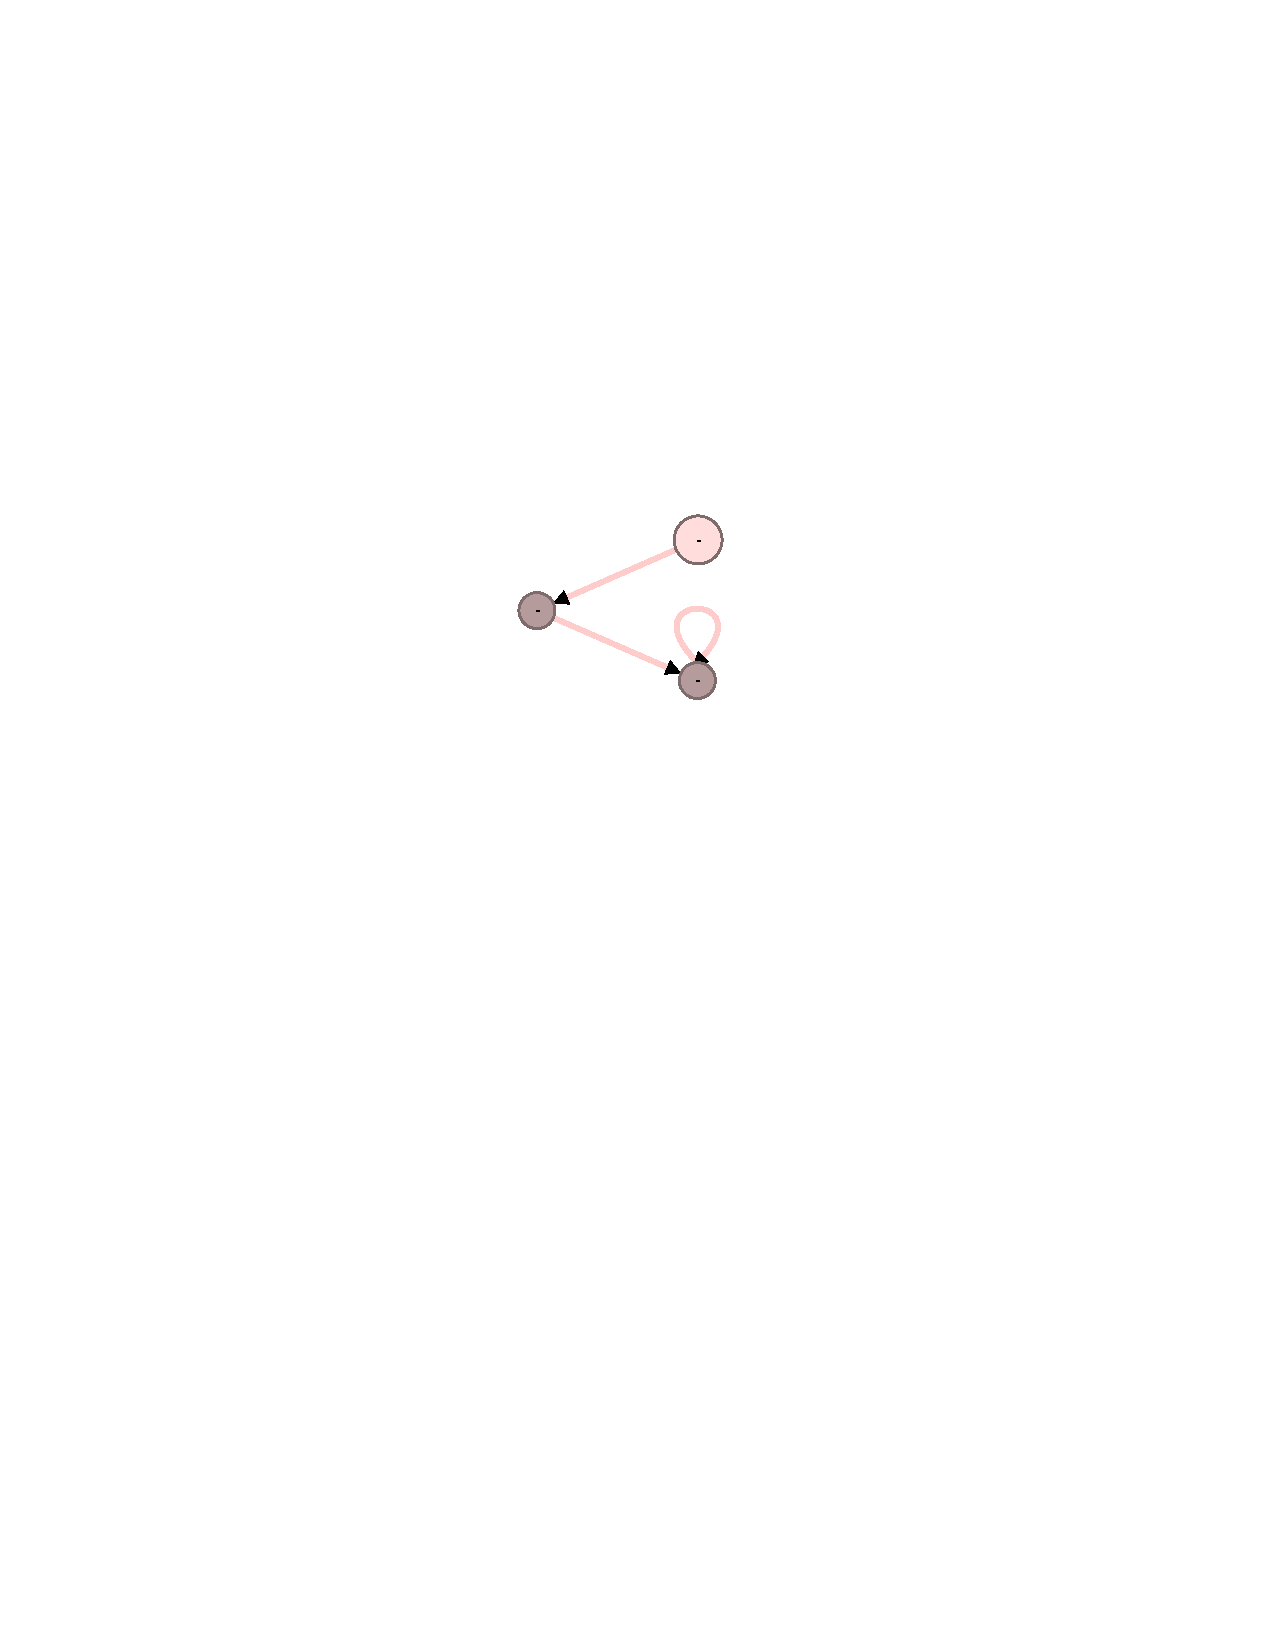
\includegraphics[width=7cm]{fig/summary2.pdf}
  \caption{The pattern on the left has three nodes, one of which is selected. On pressing the S key, it becomes a summary node, indicated by the larger size in the pattern on the right.}
  \label{fig:summary-nodes}
\end{figure}

\section{User Interaction}
The generated patterns are used by the \verifier algorithm as candidates for annotating vertices in the program unwinding tree. The following steps describe how interaction with the user works. We will later elaborate the same with an example.

\begin{enumerate}
  \item At any point, interaction with the Oracle (human user) is limited to requested patterns for a single vertex of the program unwinding tree.
  \item Start with $H^{+} = H^{-} = \{\}$. At this point, the user can provide an arbitrary pattern to begin with.
  \item If the pattern (we call it $C$) is such that $\forall h \in H^{+}, h \matchedby C$ and $\forall h \in H^{-}, h \not \matchedby C$, then C is sent to the verifier. On the other hand, if there is any heap in the existing sets $H^{+}, H^{-}$ for which these conditions are not satisfied, it is highlighted to the user.
  \item If the pattern is accepted in \autoref{alg:newcandidate}, then no more input is requested from the user.
  \item If the pattern is not accepted, one or both of $H^{+}$ or $H^{-}$ are updated, and the user needs to update the provided pattern. Return to Step 3.
\end{enumerate}

As described in \autoref{defn:heap-pat}, each individual heap can also be presented as a pattern that represents exactly that heap. As a result, all the individual heaps in $H^{+}$ and $H^{-}$ are also patterns, but with limited properties and and no $\maybe$ assignments to variables and edges, and no summary nodes. We now present an example to illustrate how the above steps work.

\subsection{Illustrating User Interaction}
\label{sec:illustrating-user-interaction}
We note that all heaps have a special \nilconst node, which represents the \nullconst address. \nilconst nodes cannot be summary nodes, and have no outgoing edges. In this example, we consider the program \altlistsimplified in \autoref{fig:alt-list-simplified} that creates a linked list with alternating $\true$ and $\false$ values for the predicate $p$.

\begin{figure}
  \centering
  \begin{Verbatim}[commandchars=\\\{\},codes={\catcode`\$=3\catcode`\^=7\catcode`\_=8}]
\PY{k+kt}{void} \PY{n+nf}{alt\PYZus{}list}\PY{p}{(}\PY{p}{)} \PY{p}{\PYZob{}}
  \PY{k+kt}{bool} \PY{n}{d} \PY{o}{=} \PY{n}{TRUE}\PY{p}{;}
  \PY{n}{List} \PY{n}{l} \PY{o}{=} \PY{n}{cons}\PY{p}{(}\PY{n}{d}\PY{p}{,} \PY{n}{NIL}\PY{p}{)}\PY{p}{;}
  \PY{c+c1}{// LOOP\PYZhy{}CONS: build a list with alternating Boolean values.}
  \PY{k}{while} \PY{p}{(}\PY{n}{non\PYZus{}det}\PY{p}{(}\PY{p}{)}\PY{p}{)} \PY{p}{\PYZob{}}
    \PY{n}{d} \PY{o}{=} \PY{o}{!}\PY{n}{d}\PY{p}{;}
    \PY{n}{l} \PY{o}{=} \PY{n}{cons}\PY{p}{(}\PY{n}{d}\PY{p}{,} \PY{n}{l}\PY{p}{)}\PY{p}{;}
  \PY{p}{\PYZcb{}}
  \PY{c+c1}{// LOOP\PYZhy{}CHK: check that the Boolean values alternate.}
  \PY{k}{while} \PY{p}{(}\PY{n}{l} \PY{o}{!}\PY{o}{=} \PY{n}{NIL}\PY{p}{)} \PY{p}{\PYZob{}}
    \PY{n}{assert}\PY{p}{(}\PY{n}{l}\PY{o}{\PYZhy{}}\PY{o}{\PYZgt{}}\PY{n}{data} \PY{o}{=}\PY{o}{=} \PY{n}{d}\PY{p}{)}\PY{p}{;}
    \PY{n}{d} \PY{o}{=} \PY{o}{!}\PY{n}{d}\PY{p}{;}
    \PY{n}{l} \PY{o}{=} \PY{n}{l}\PY{o}{\PYZhy{}}\PY{o}{\PYZgt{}}\PY{n}{next}\PY{p}{;}
  \PY{p}{\PYZcb{}}
  \PY{k}{return}\PY{p}{;}
\PY{p}{\PYZcb{}}
\end{Verbatim}

  \caption{\altlistsimplified: a slightly modified and simplified version of the SV-COMP benchmark program \altlist (\autoref{fig:alt-list}) that constructs a list with cells that store alternating Boolean values for a known predicate. We will demonstrate concrete heaps and patterns for the prgram location at the label \checkpoint.}
  \label{fig:alt-list-simplified}
\end{figure}

The user is not expected to know what the program or the verification algorithm does, and will only be presented with examples. User insight is expected based solely on those. We assume that only a single predicate $p \in \predvars$ exists, so all node colors only refer to that single predicate. We start with $H^{+} = H^{-} = \{\}$, at which point the user can't really provide any insight. It might be worthwhile to have a default candidate be provided by the interface itself at this point, but we still leave it to the user just in case they have additional insight about the program from other sources. Suppose the user just provides a pattern with a single node labeled \nilconst (\autoref{fig:nil-node}).

% Just the nil node.
\begin{figure}
  \centering
  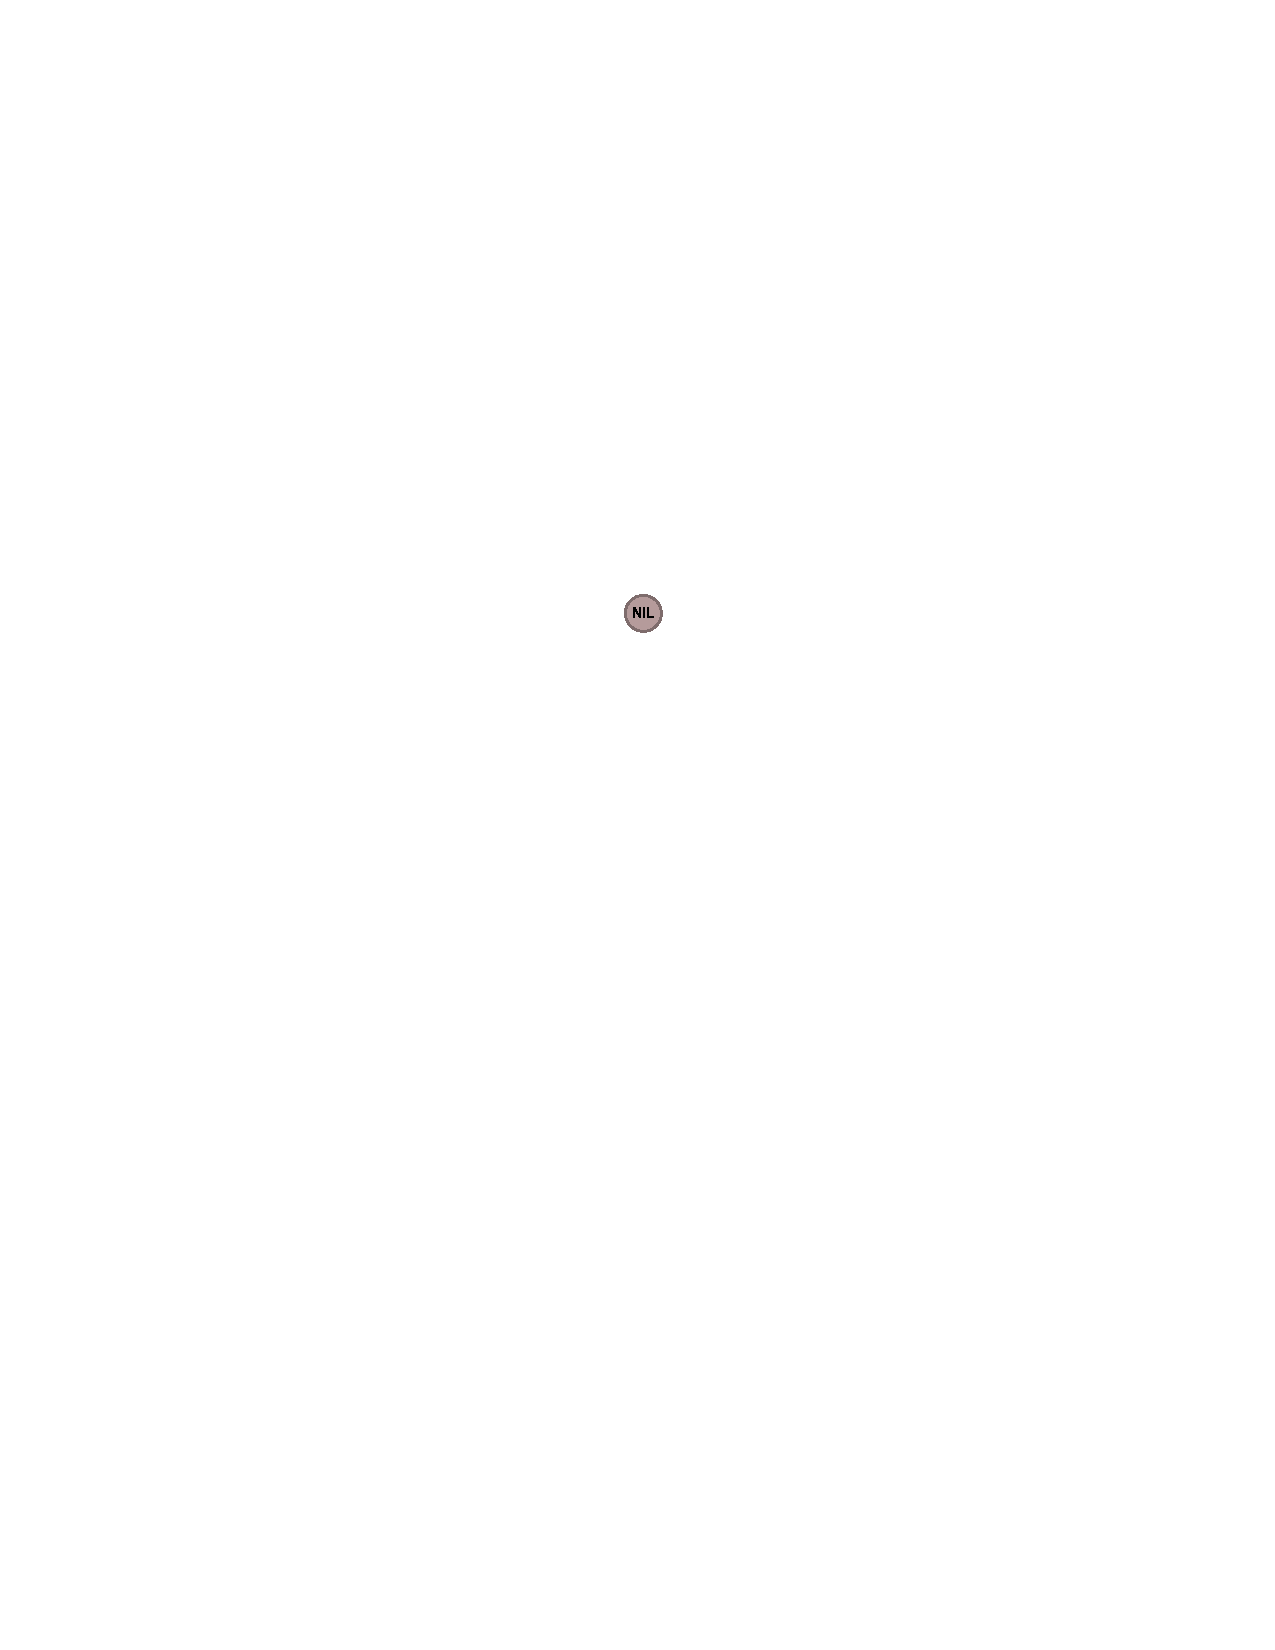
\includegraphics[width=5cm]{fig/just-nil.pdf}
  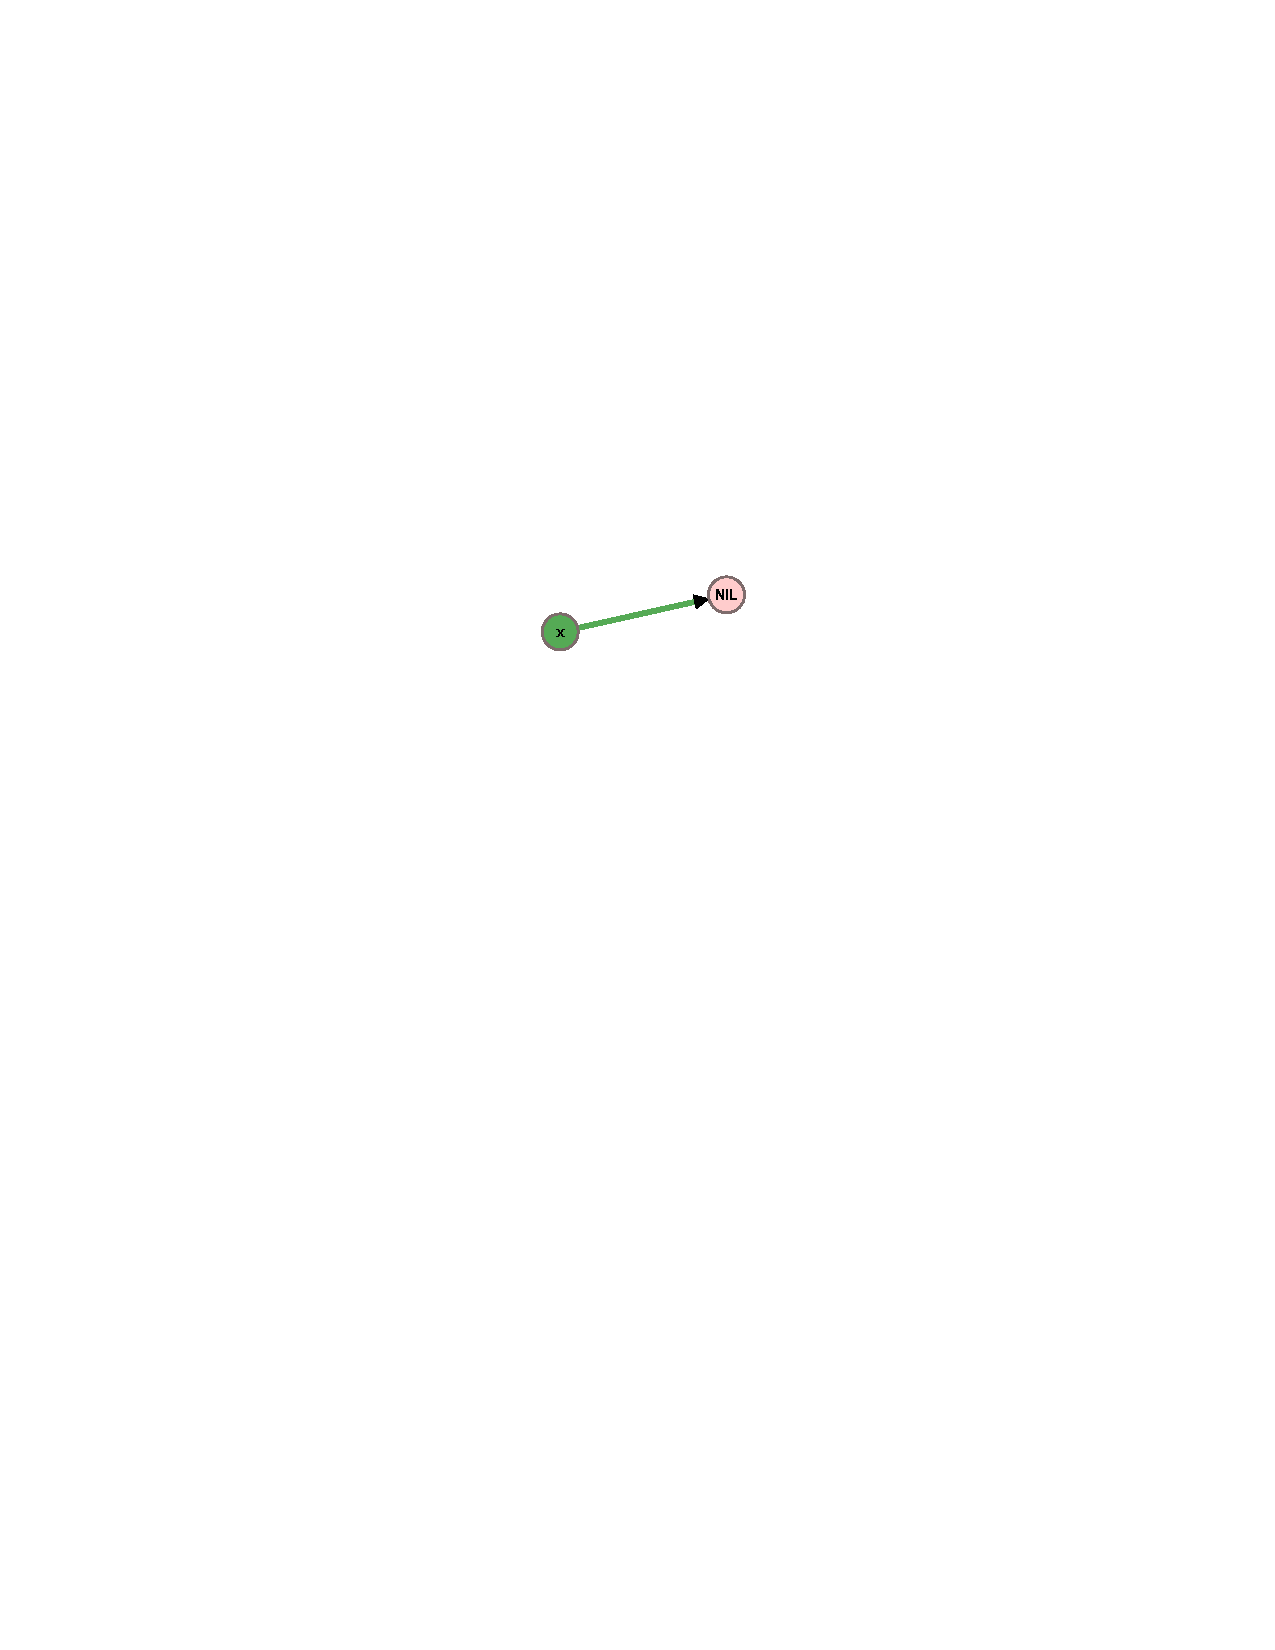
\includegraphics[width=5cm]{fig/positive1.pdf}
  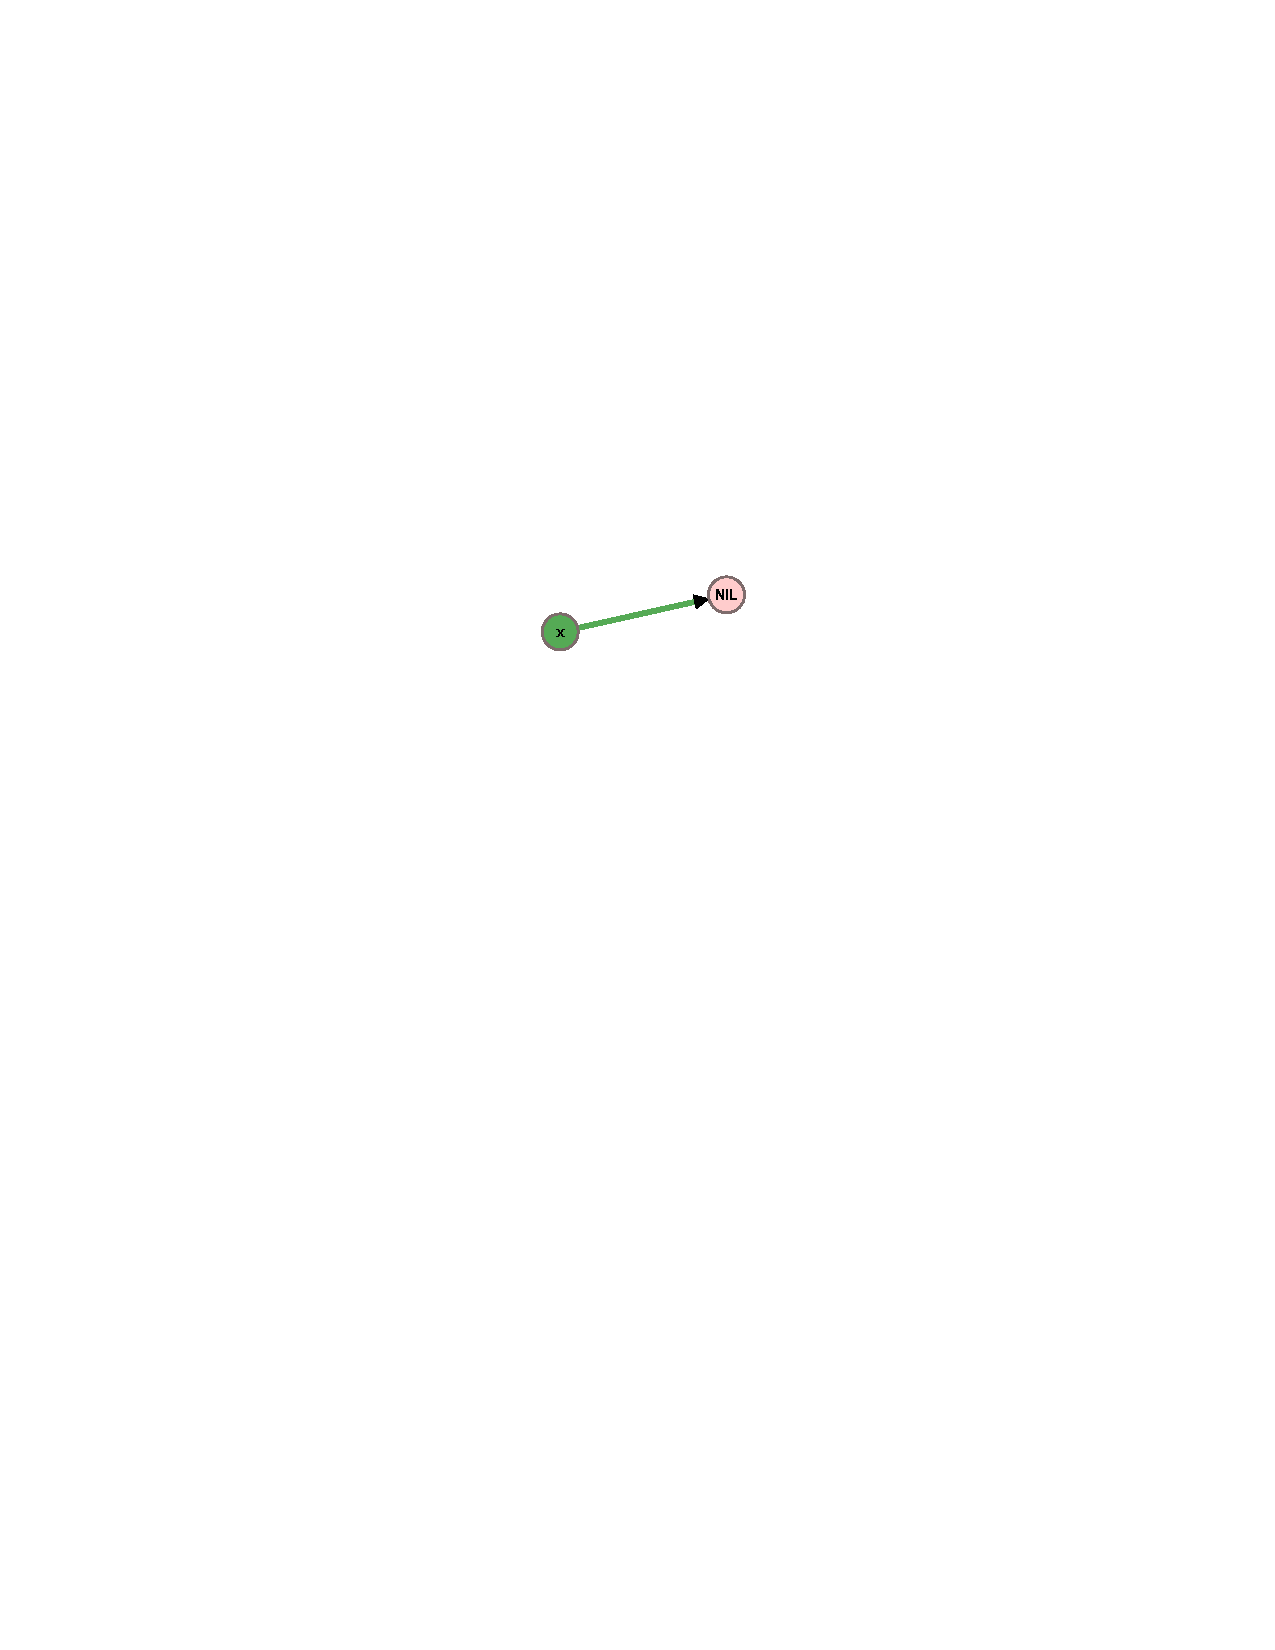
\includegraphics[width=5cm]{fig/positive1.pdf}
  \caption{On the left is the initial pattern candidate provided by the user. At this point, the user does not know what the program is doing, or what program location the candidate is being requested for. As a response, the verifier returns the concrete heap in the center as a positive example, indicating that the pattern provided by the user should be able to cover it. The user in response eagerly provides the same positive example as a candidate pattern.}
  \label{fig:nil-node}
\end{figure}

At this point, we get a new concrete heap back from the verifier (\autoref{fig:nil-node}). The user once again tries to respond in a simple way by providing the heap returned by the verifier as a pattern (\autoref{fig:nil-node}). In response to the pattern provided by the user, the verifier returns a new heap as part of $H^{+}$, shown in \autoref{fig:positive-examples}.

% Some positive examples.
\begin{figure}
  \centering
  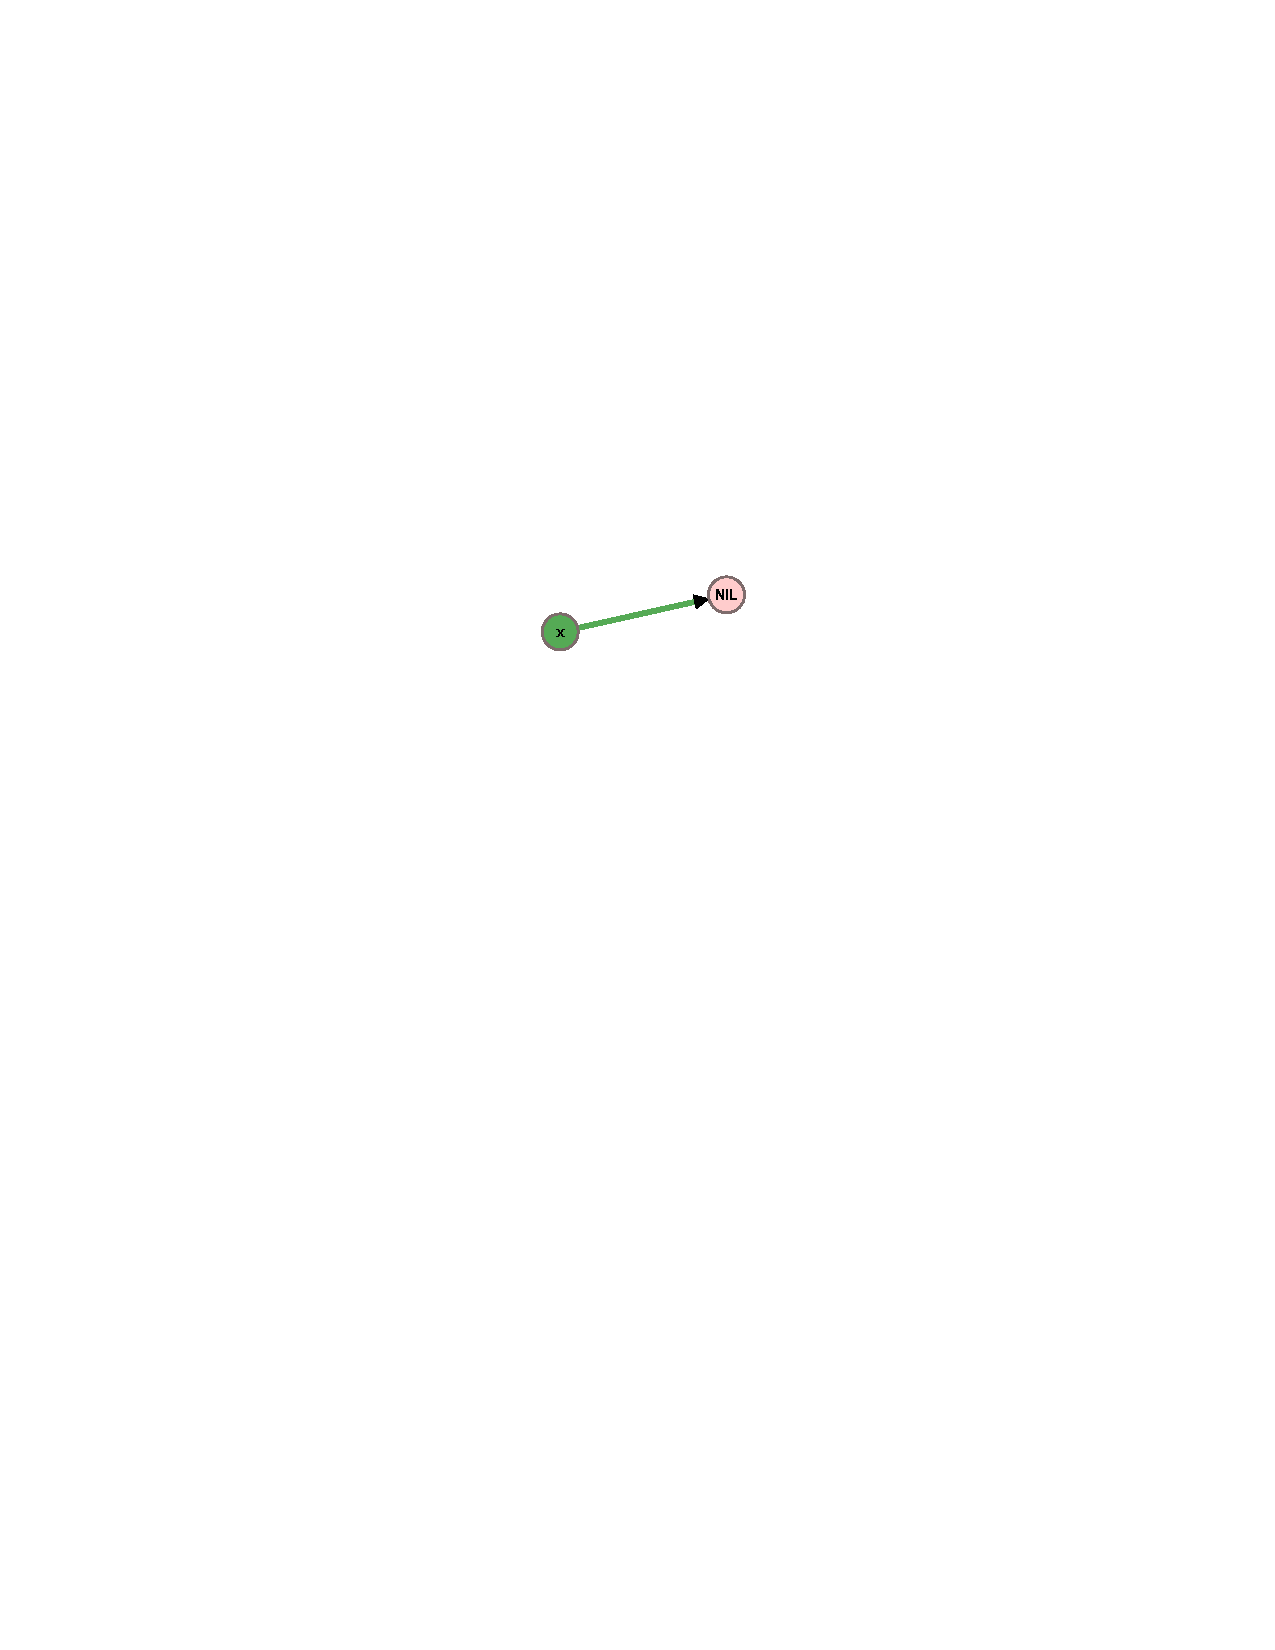
\includegraphics[width=7cm]{fig/positive1.pdf}
  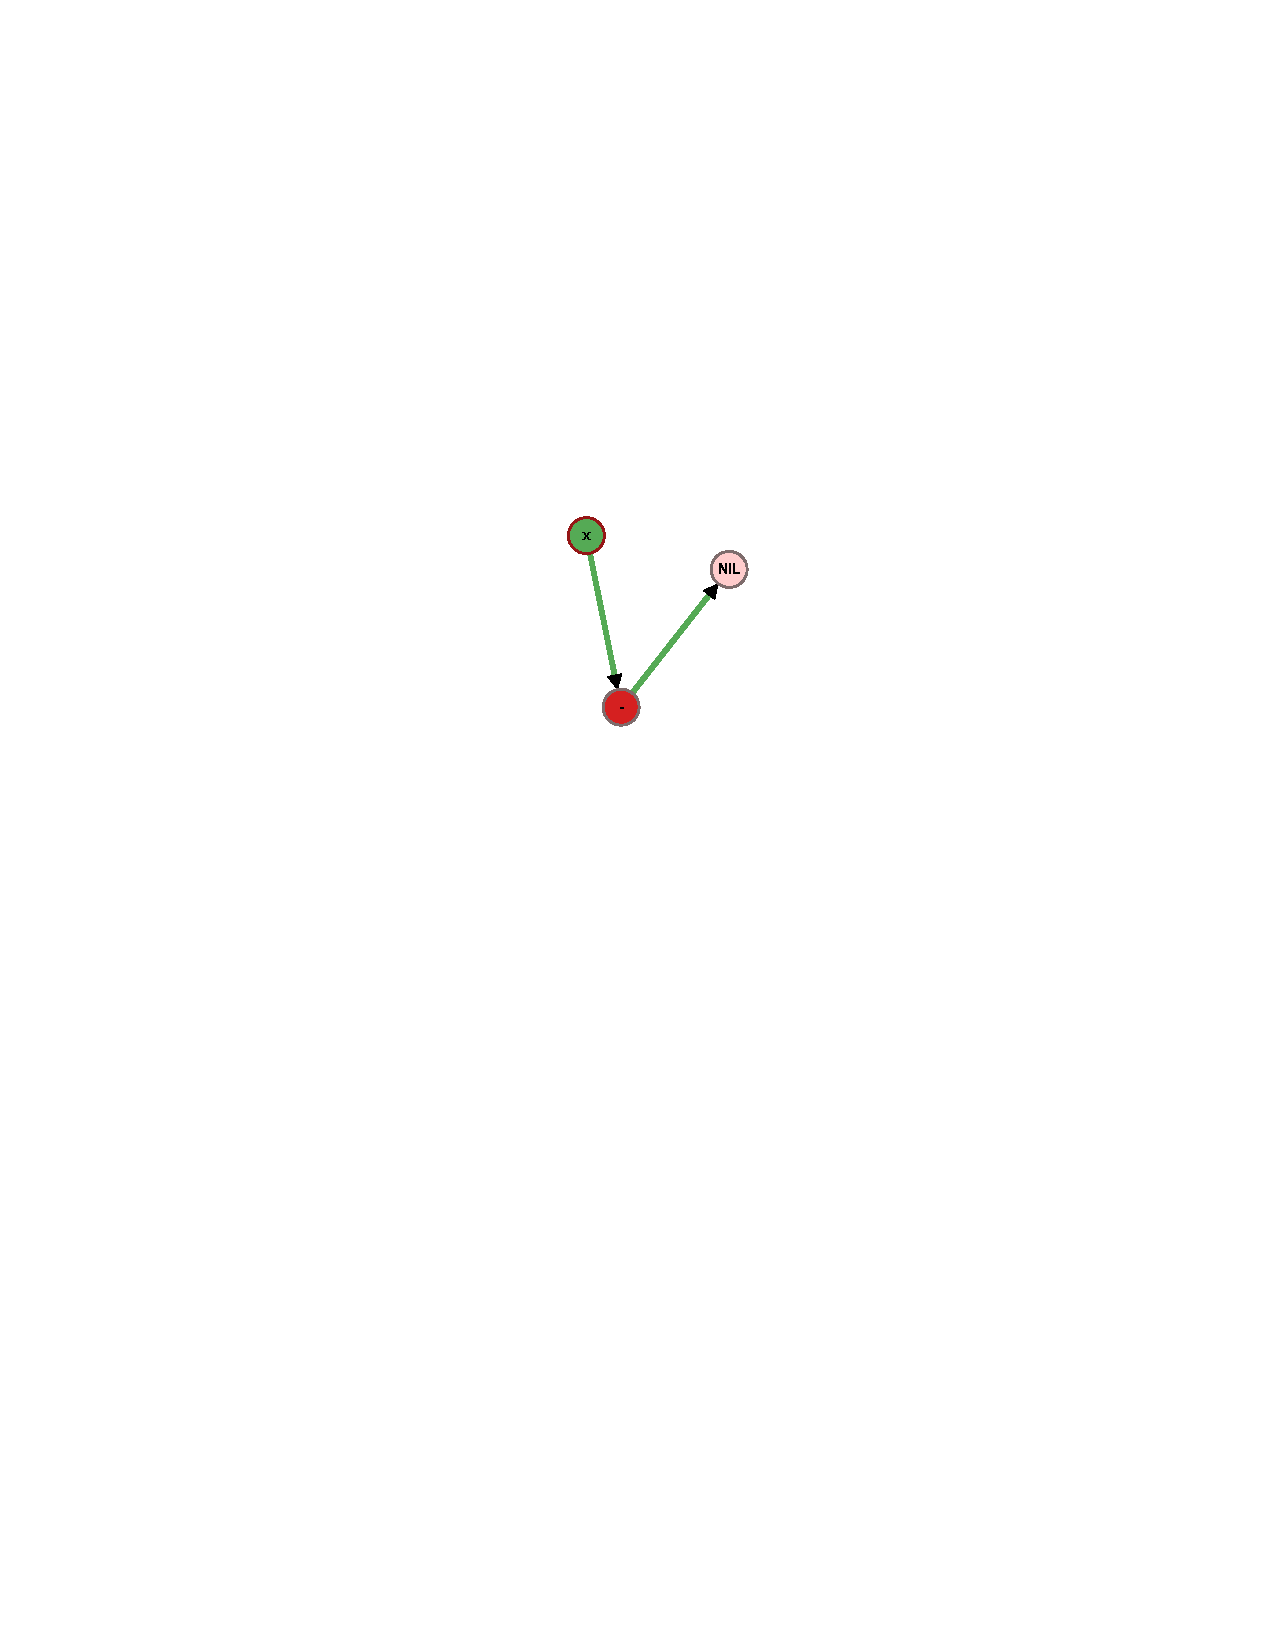
\includegraphics[width=7cm]{fig/positive2.pdf}
  \caption{The set $H^{+}$ after the user has provided two candidate patterns to the verifier.}
  \label{fig:positive-examples}
\end{figure}

Now is the first time the user needs to think of a non-trivial pattern, because the two heaps we have in $H^{+}$ are very different. At this point, the user makes two attempts, a wrong one and a right one, and we describe what happens in each case in \autoref{fig:pattern-attempts}. The right pattern uses a summary node, because summary nodes can abstract out zero or more concrete nodes. Similarly, $\maybe$ edges are used to indicate that the edge may or may not actually exist in a concrete pattern represented by the heap pattern.

% Some candidates.
\begin{figure}
  \centering
  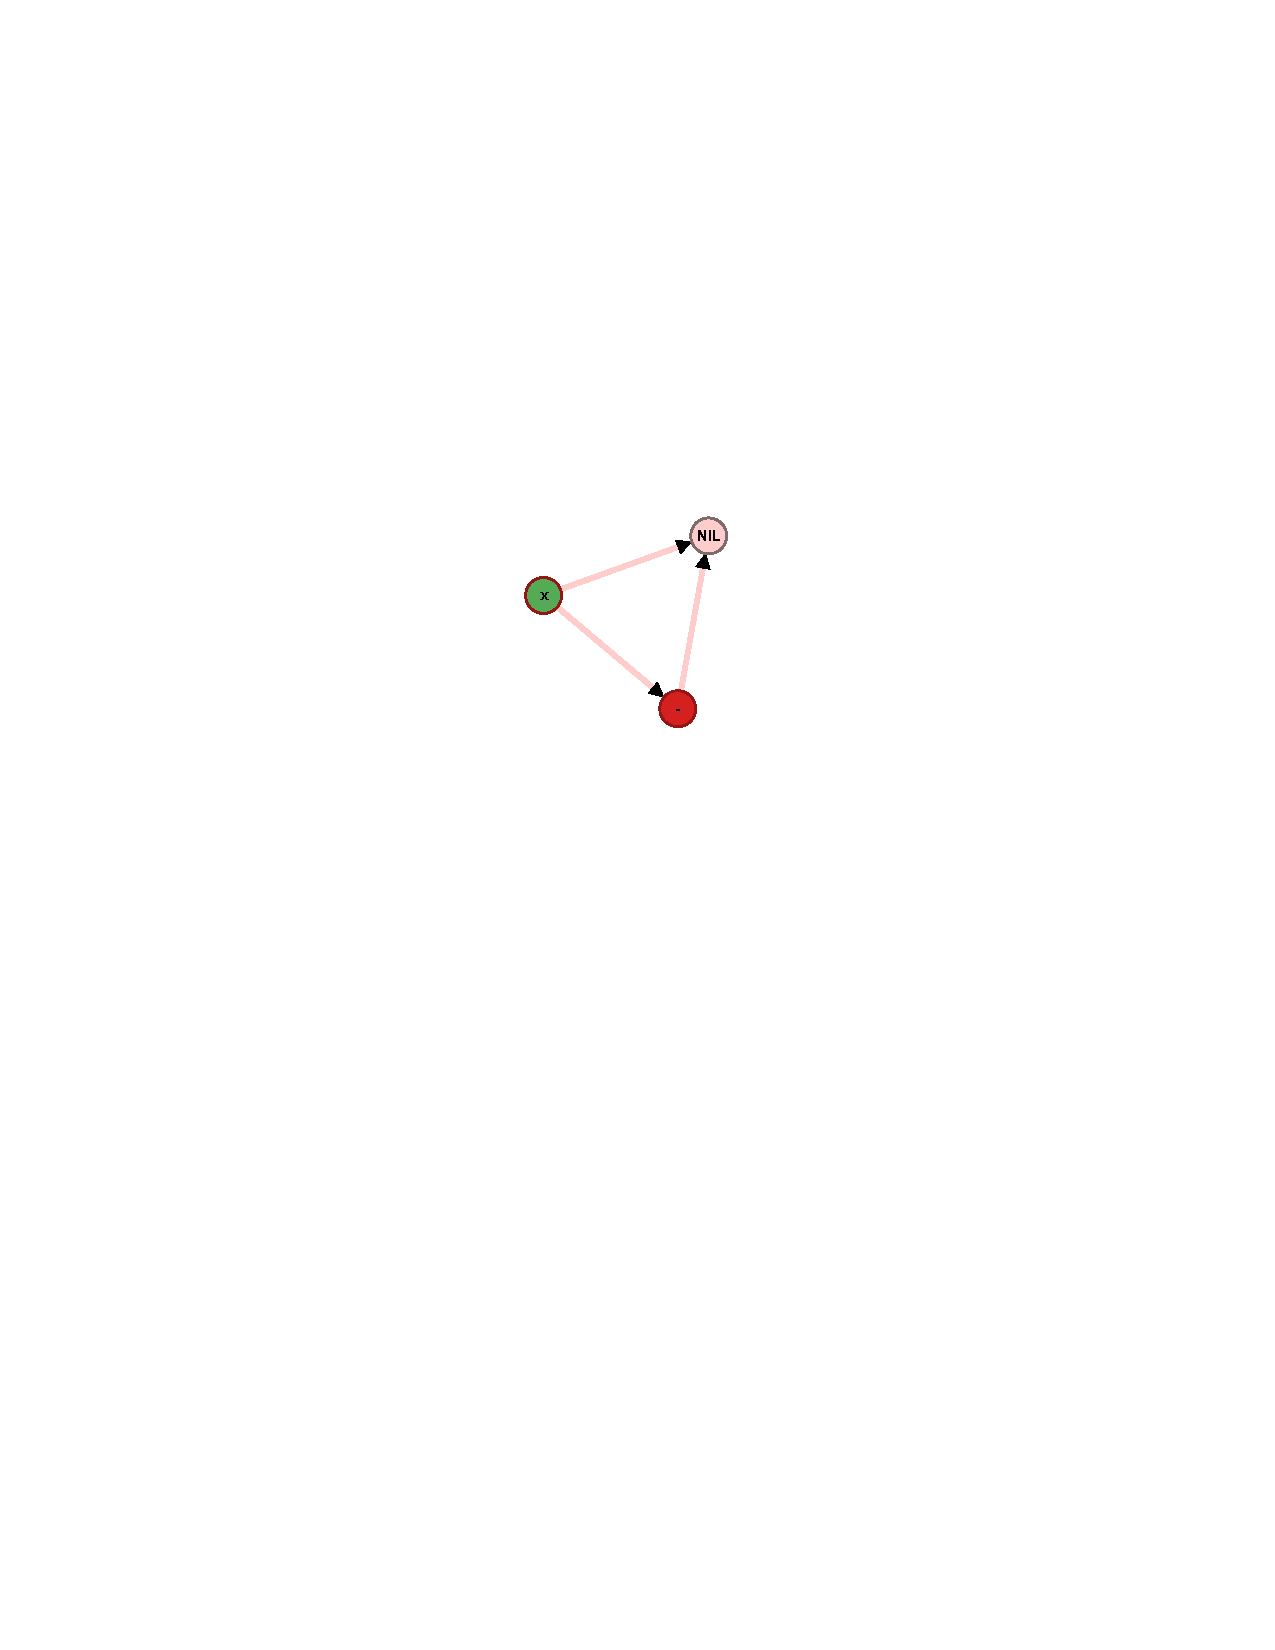
\includegraphics[width=7cm]{fig/candidate3.pdf}
  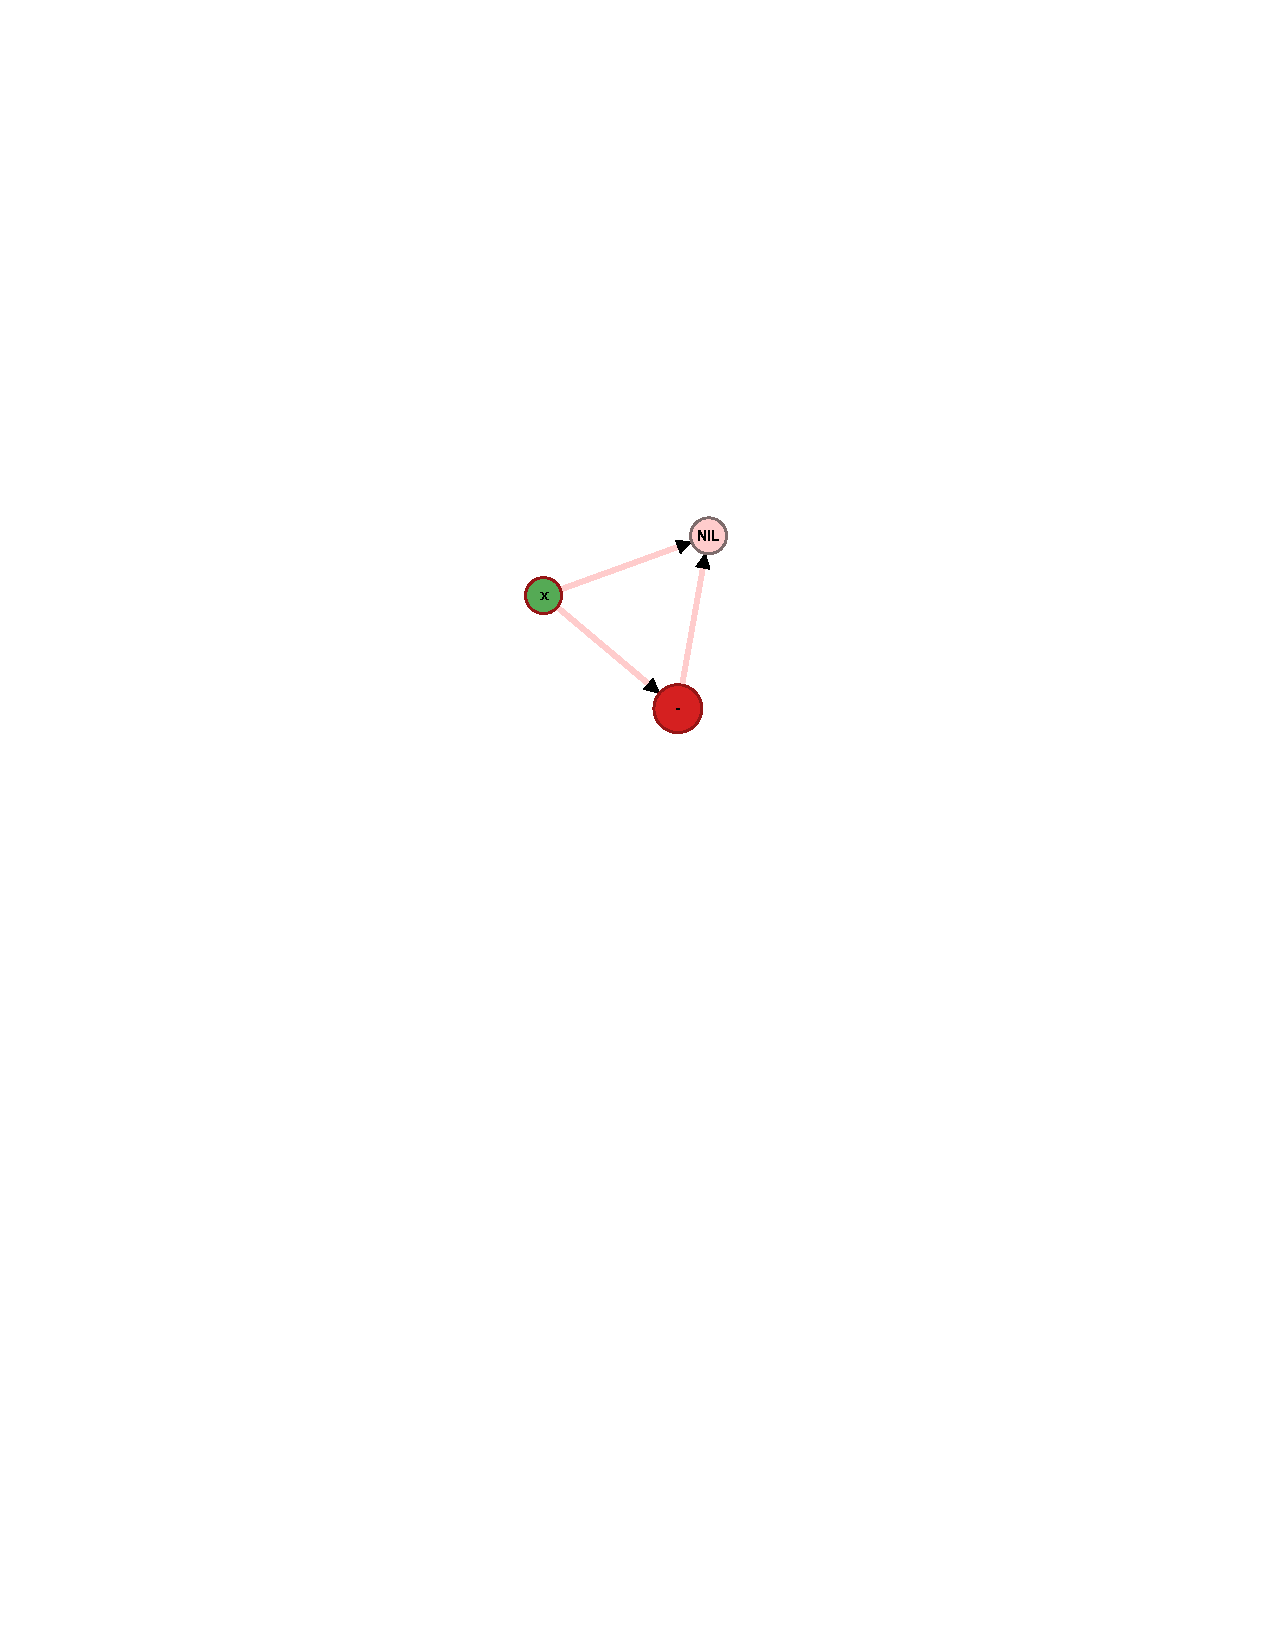
\includegraphics[width=7cm]{fig/candidate4.pdf}
  \caption{The user first provides the pattern on the left as a candidate. But we note that this pattern does not actually cover the first heap in $H^{+}$ in \autoref{fig:positive-examples}, so the interface highlights the first heap, and the user has to correct their input. After making one of the nodes a summary node (indicated by the larger size in the pattern on the right), the pattern starts to be entailed by both our heaps in $H^{+}$, and the interface passes it on to the verifier.}
  \label{fig:pattern-attempts}
\end{figure}

After several back and forth interactions with the verifier, we might end up in a state where we have several positive examples, as shown in in \autoref{fig:several-positive-examples}. The user now begins to get an idea of what the program might actually be doing at this program location. It looks like the program constructs ``alternating'' linked lists that always start with a node where the predicate is $\true$. The heap variable $x$ acts as the head of the list.

% Some positive examples.
\begin{figure}
  \centering
  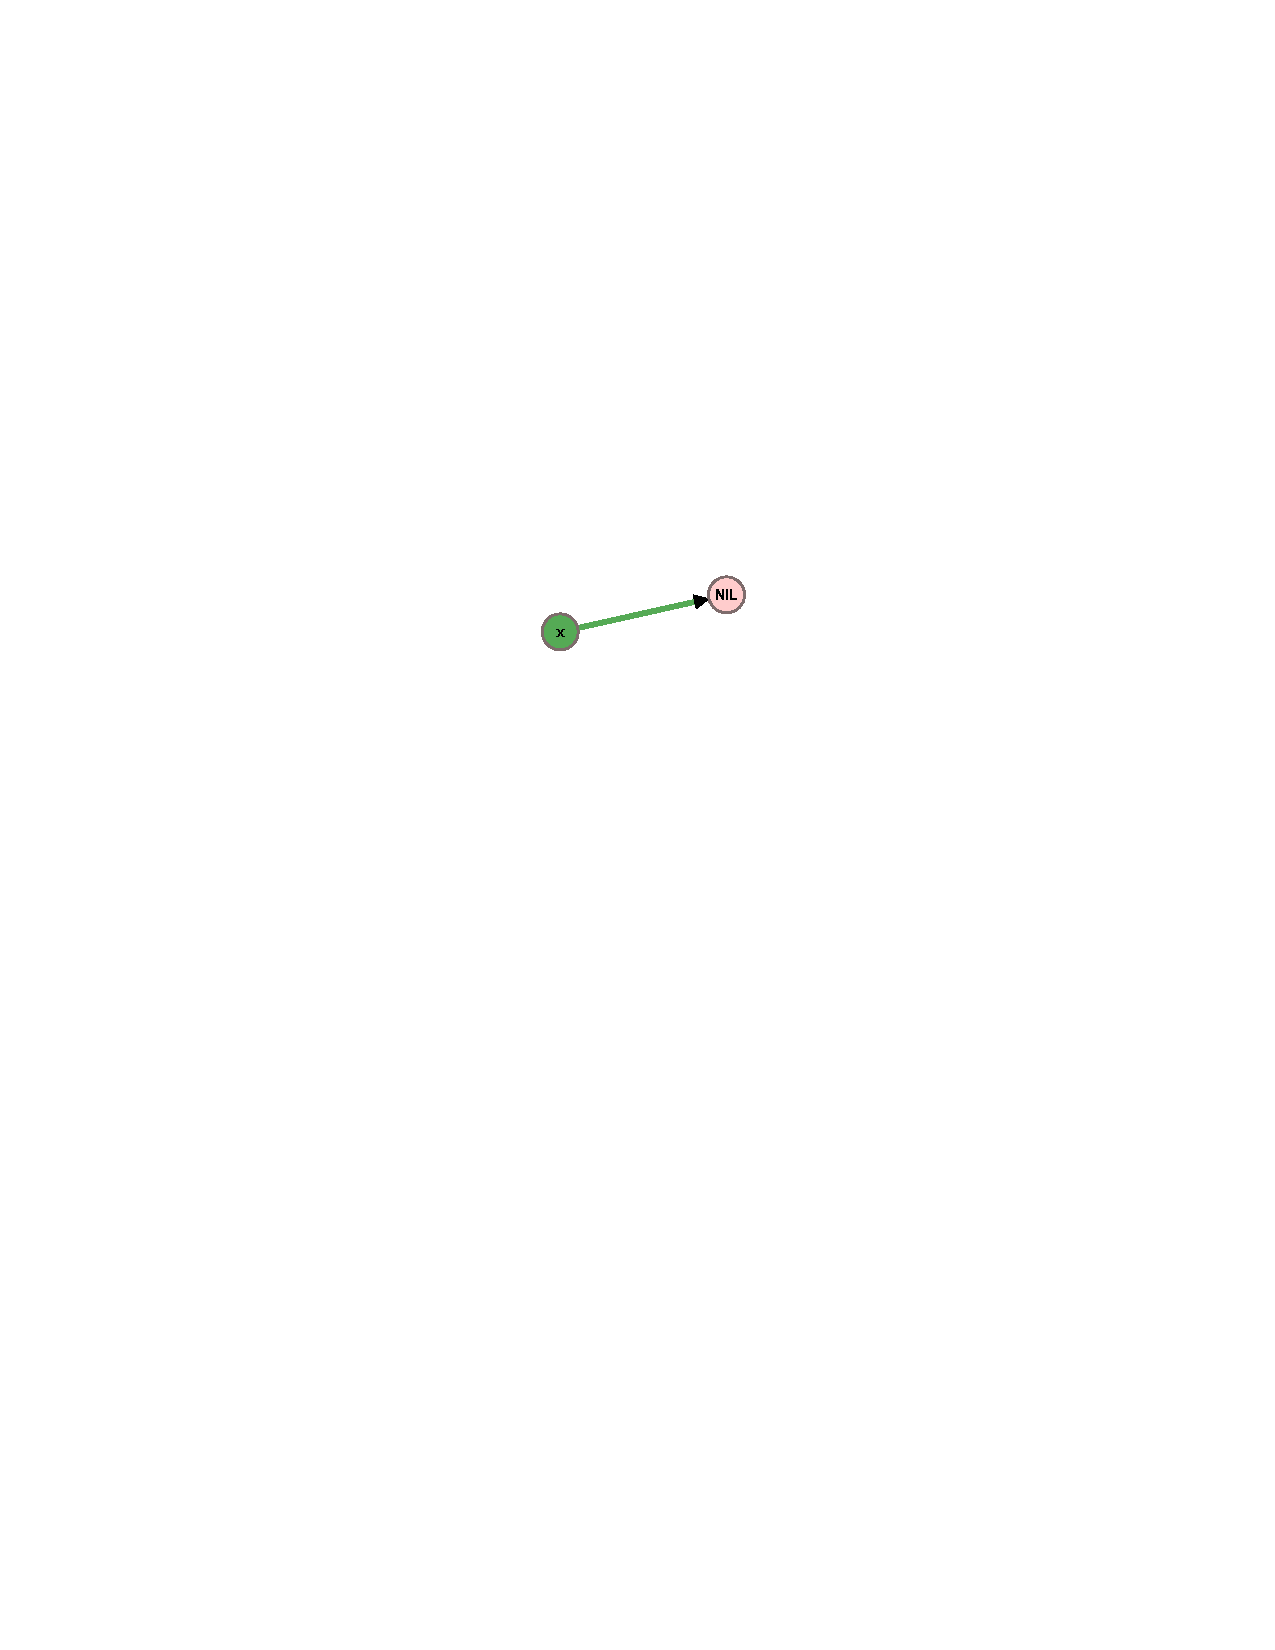
\includegraphics[width=5cm]{fig/positive1.pdf}
  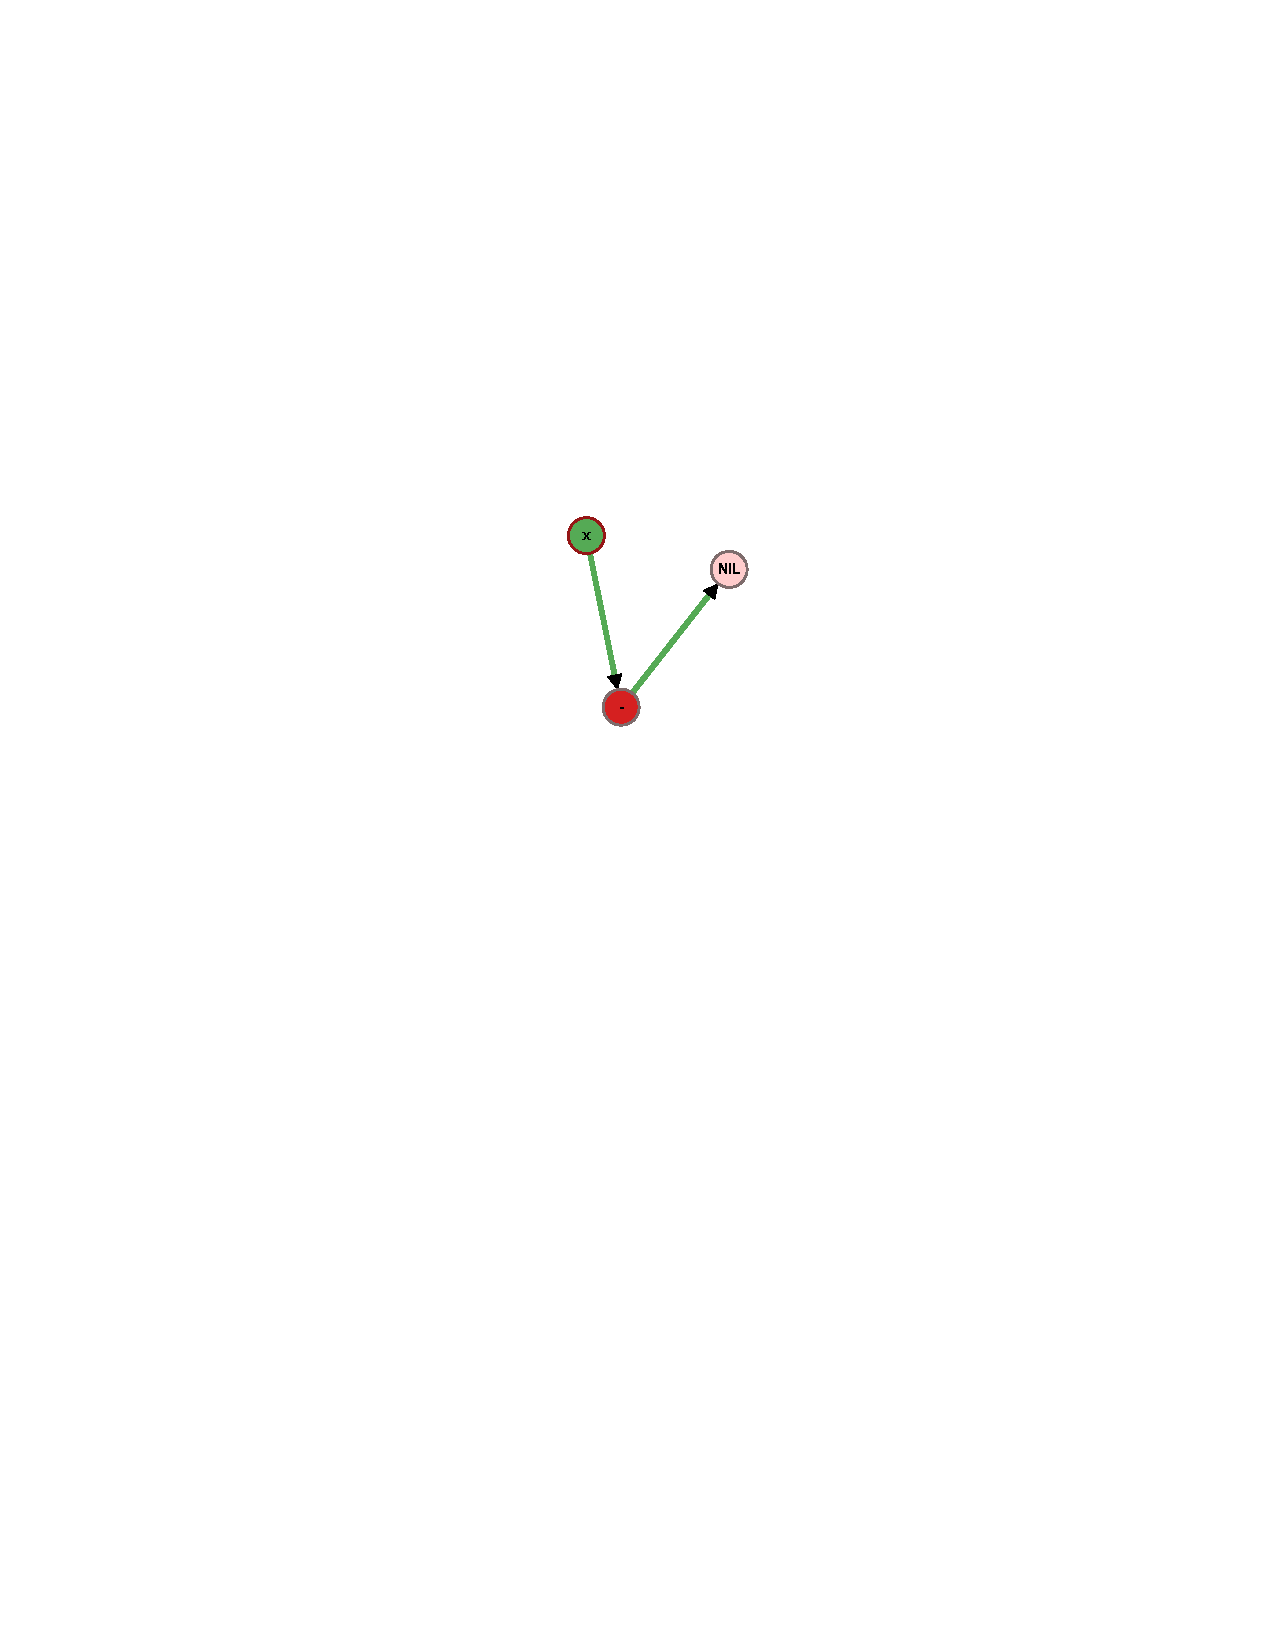
\includegraphics[width=5cm]{fig/positive2.pdf}
  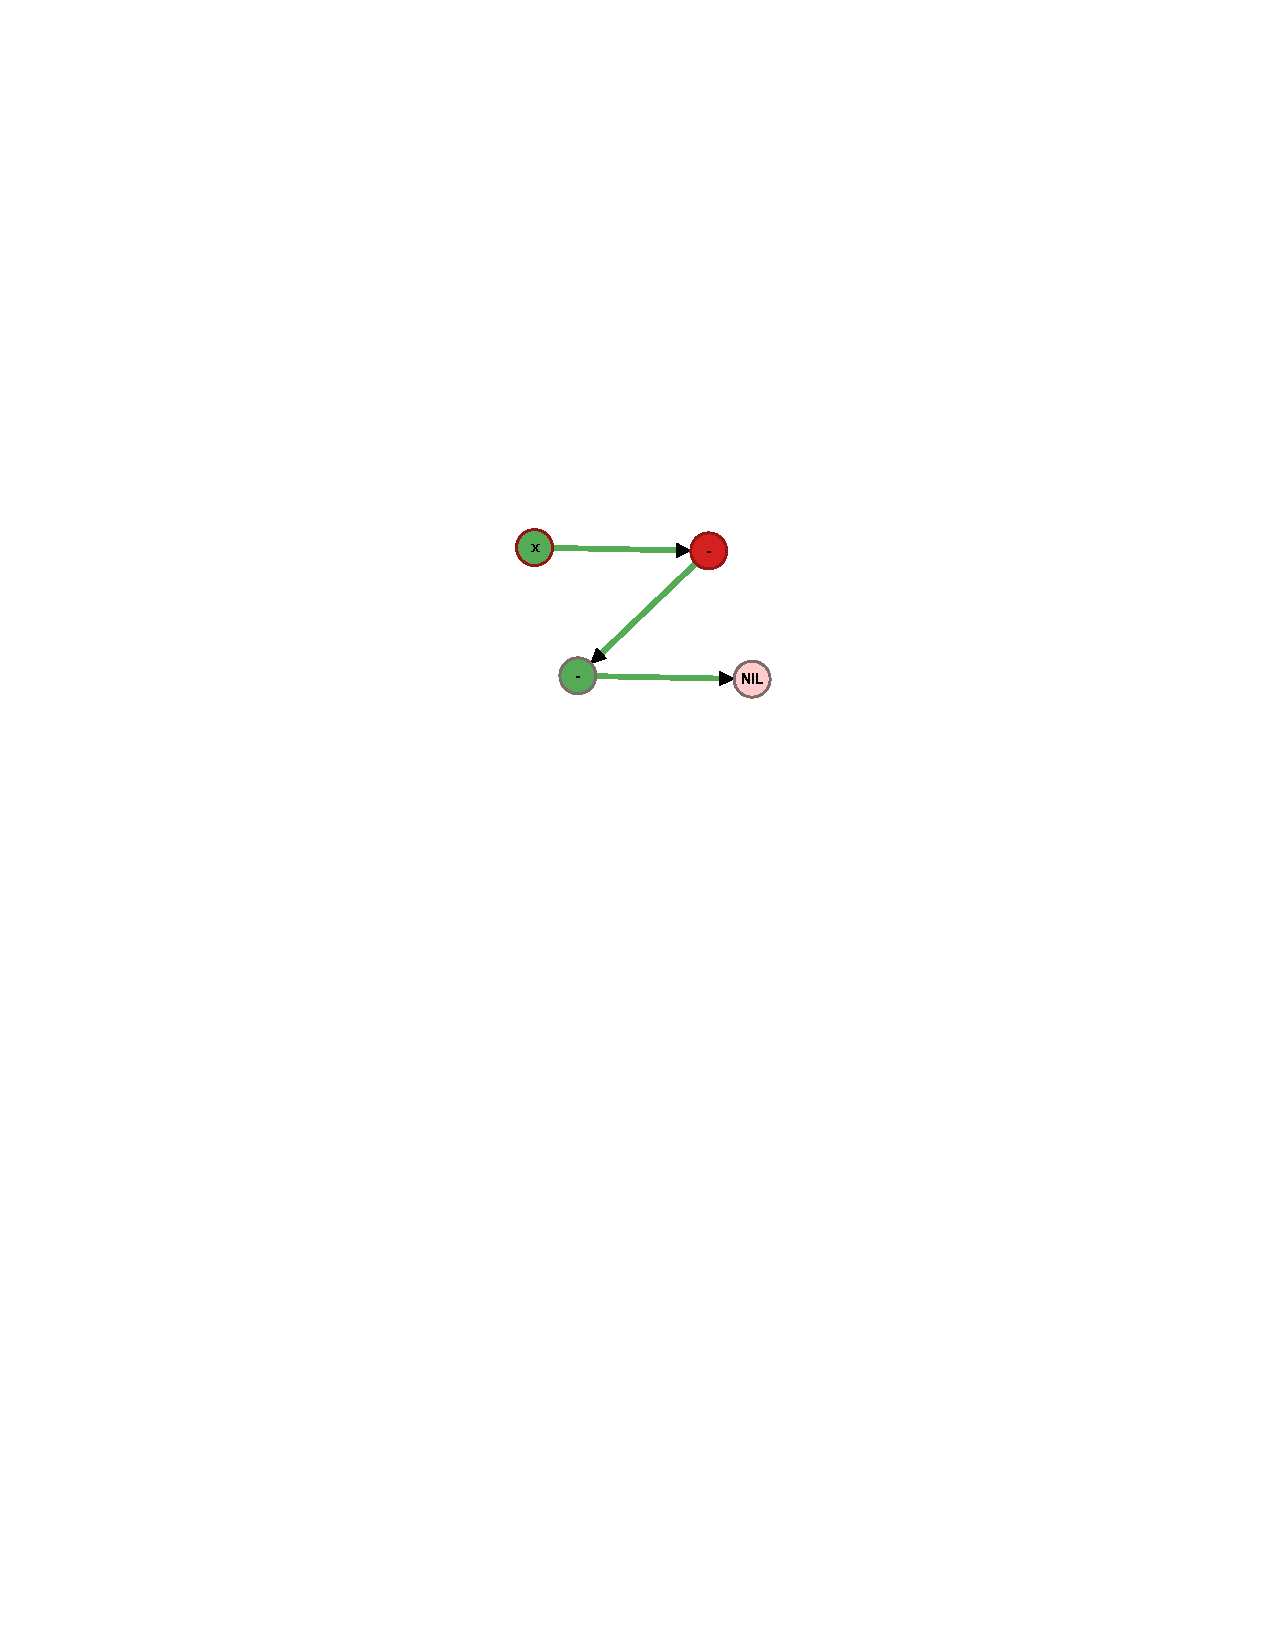
\includegraphics[width=5cm]{fig/positive3.pdf}
  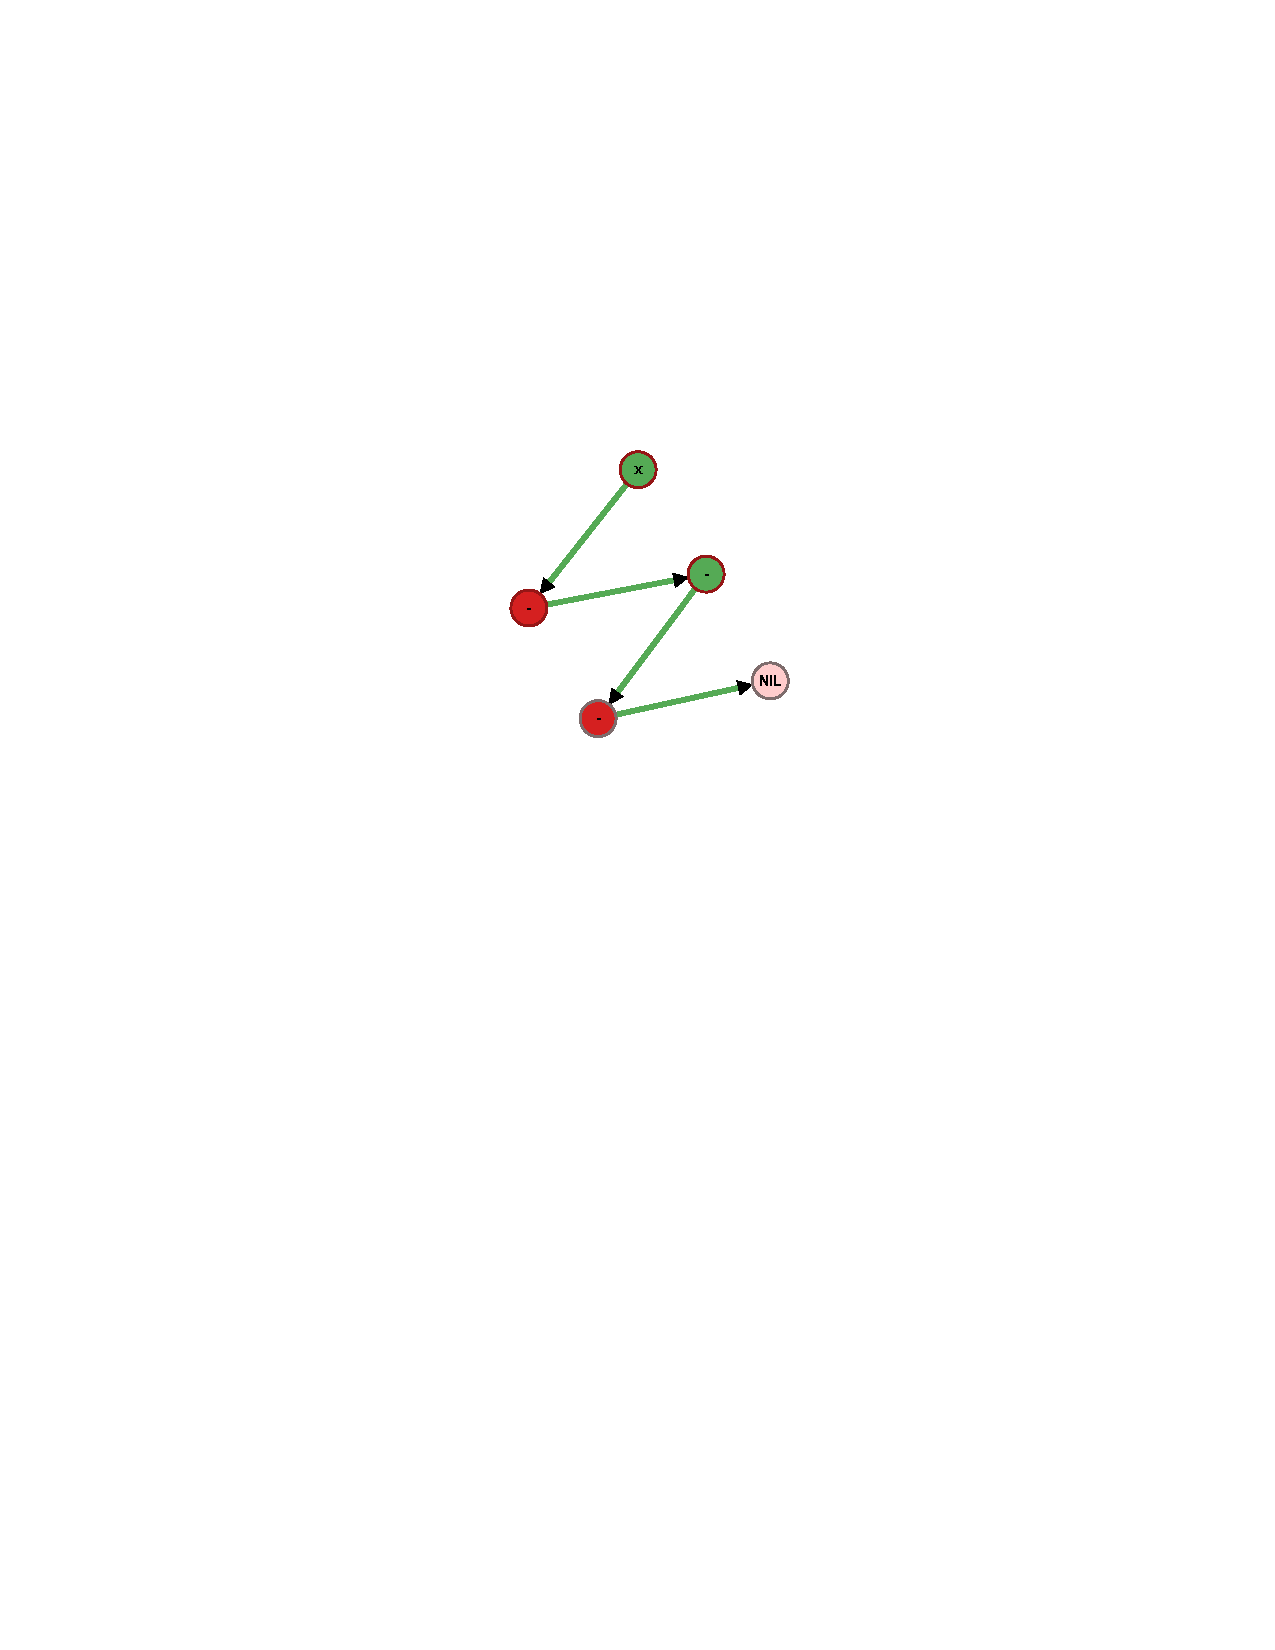
\includegraphics[width=5cm]{fig/positive4.pdf}
  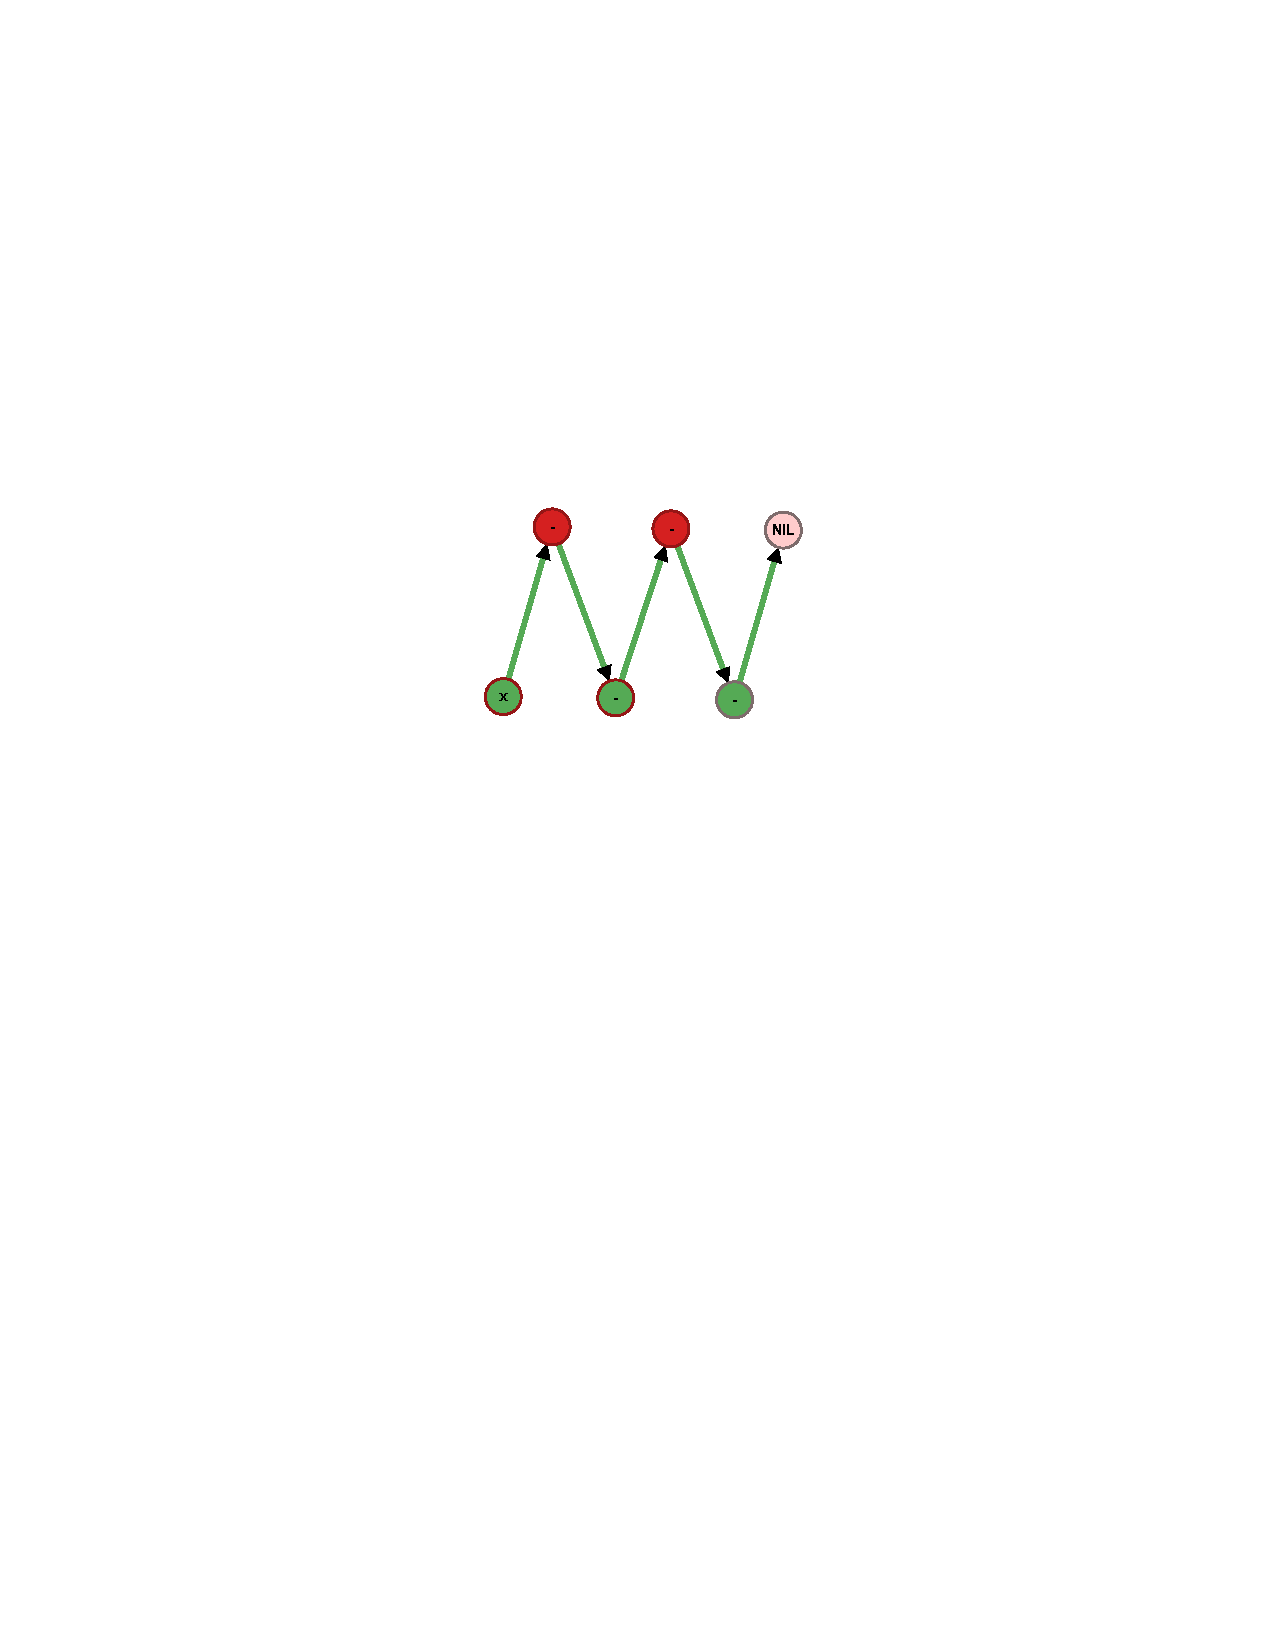
\includegraphics[width=5cm]{fig/positive5.pdf}
  \caption{The set $H^{+}$ of positive examples, after a few back and forth interactions between the user and the verifier. Note that a suitable candidate has still not been found, and $H^{-}$ is still empty.}
  \label{fig:several-positive-examples}
\end{figure}

After seeing all these examples, the user submits the pattern in \autoref{fig:almost-right-pattern}, hoping that it would be accepted by the verifier. It might well be, depending on what state the verifier is in. But in our example, the pattern provided by the user turns out to be too general, and the verifier returns a negative example for the first time. Finally, $H^{-}$ is non-empty, as looks as shown in \autoref{fig:negative-example}. Picking up on this, the user makes a correction, submitting the pattern in \autoref{fig:right-pattern}, which is finally accepted by the verifier.

% Almost right pattern.
\begin{figure}
  \centering
  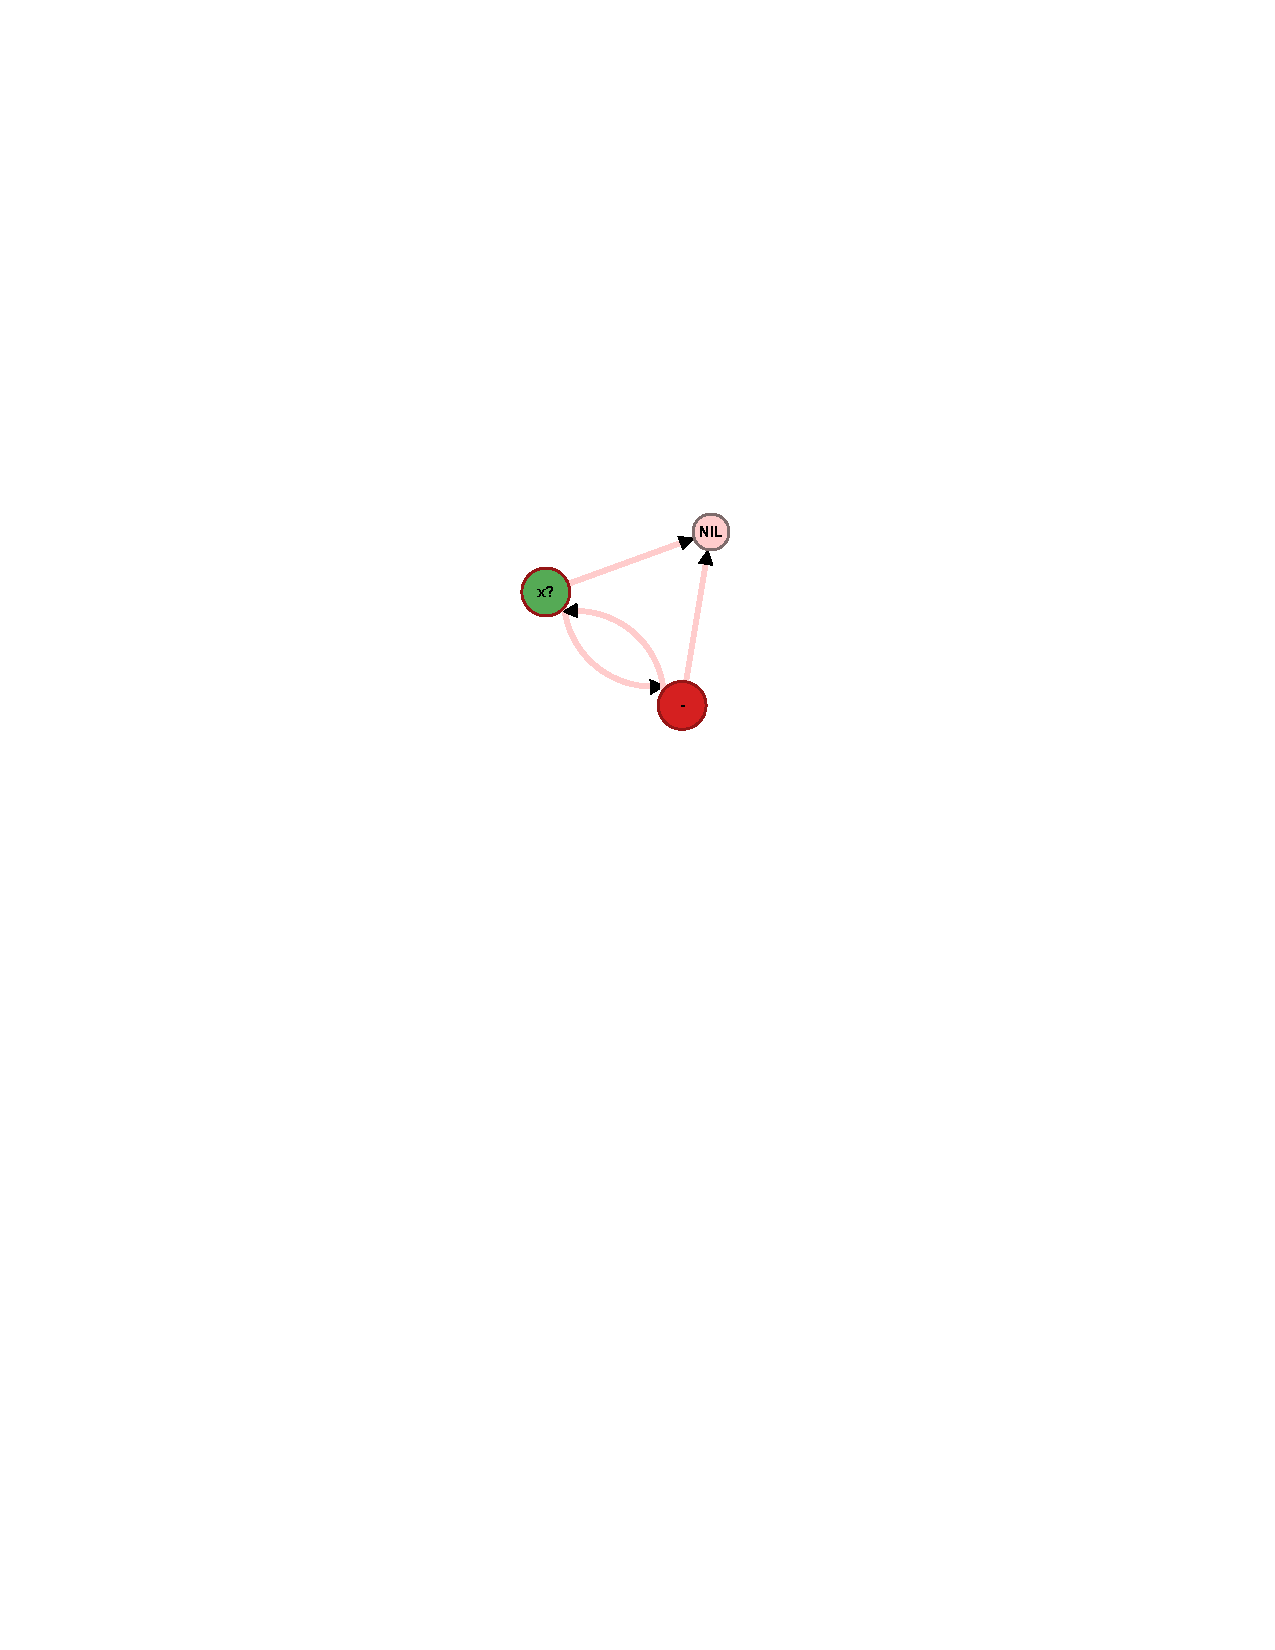
\includegraphics[width=7cm]{fig/candidate5.pdf}
  \caption{This candidate pattern is almost right, it captures the alternating list property, but has a problem that results in a negative example, shown in \autoref{fig:negative-example}.}
  \label{fig:almost-right-pattern}
\end{figure}

% Negative example.
\begin{figure}
  \centering
  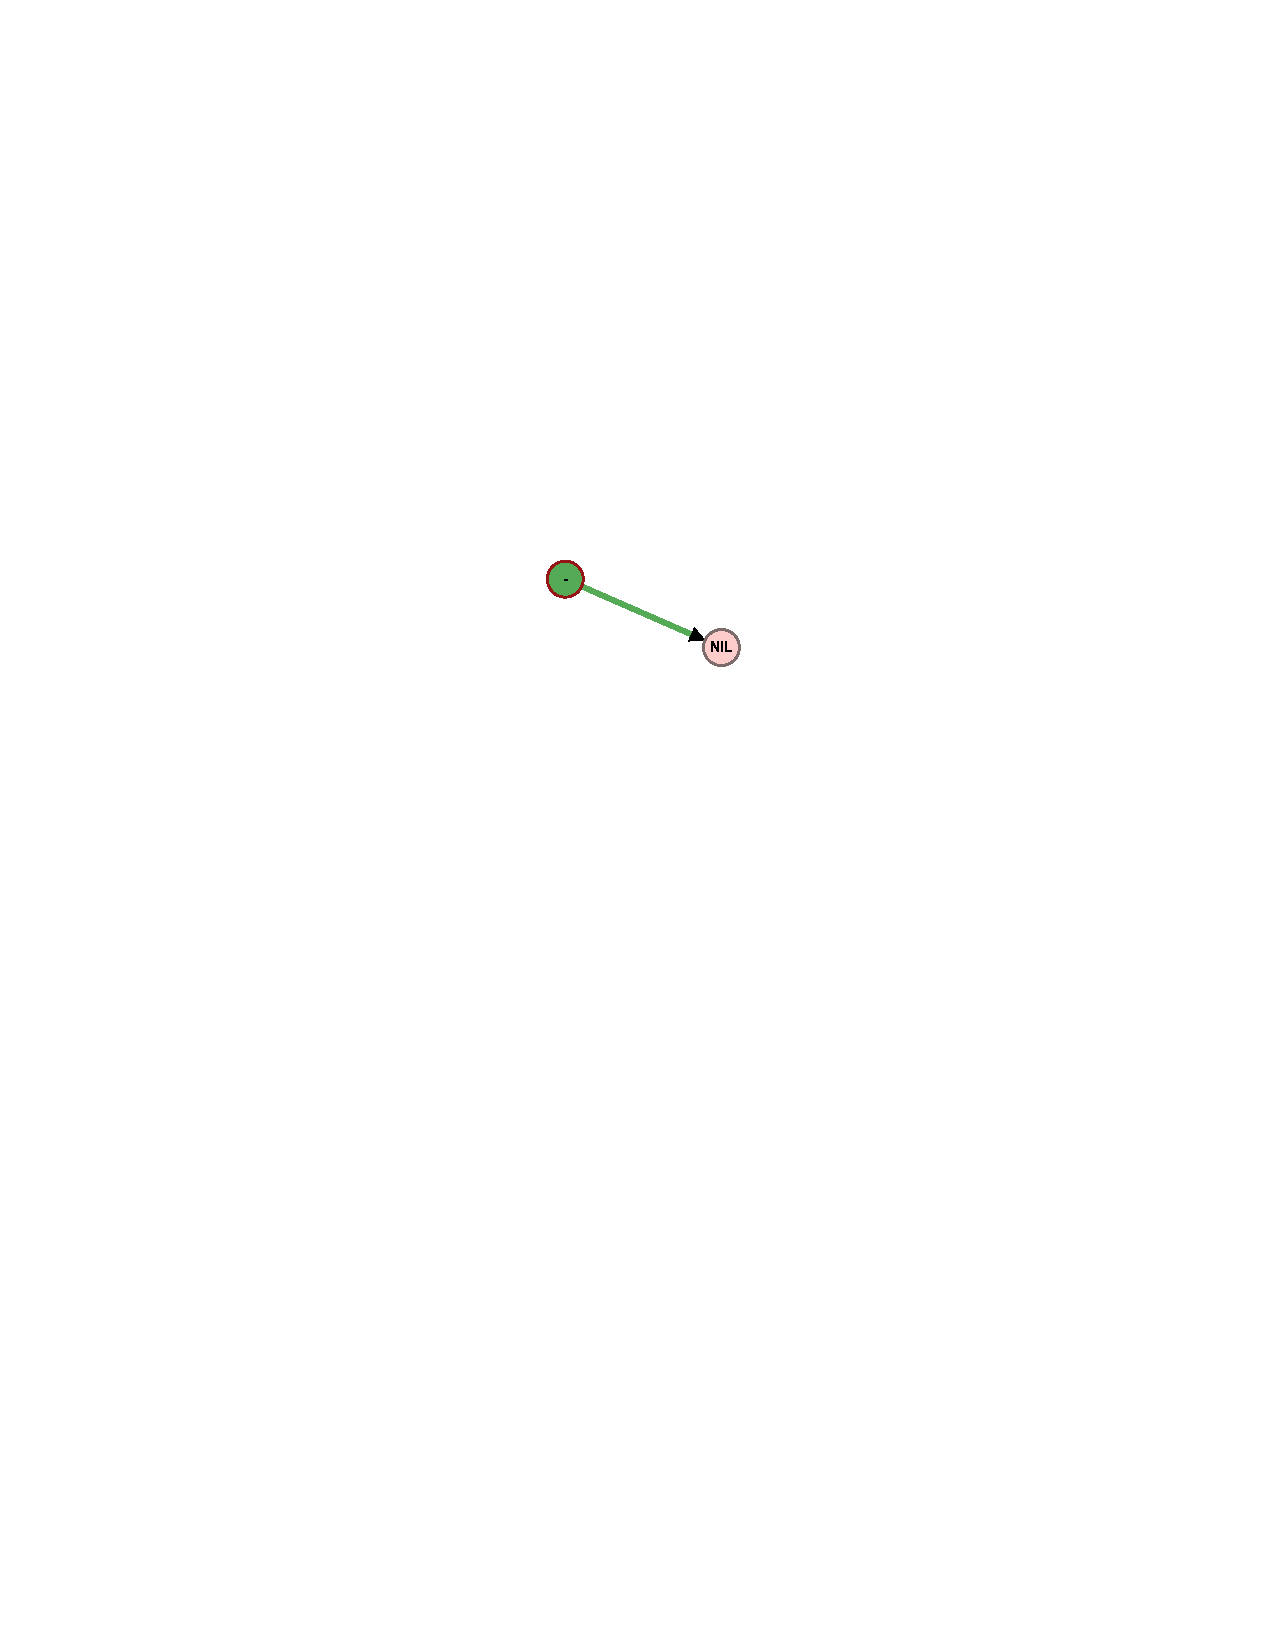
\includegraphics[width=7cm]{fig/negative1.pdf}
  \caption{The set $H^{-}$, with a simple heap that indicates that the first node does not have $x$ pointing to it. This heap is allowed by the pattern in \autoref{fig:almost-right-pattern}, but not by the pattern in \autoref{fig:right-pattern}.}
  \label{fig:negative-example}
\end{figure}

% Final right pattern.
\begin{figure}
  \centering
  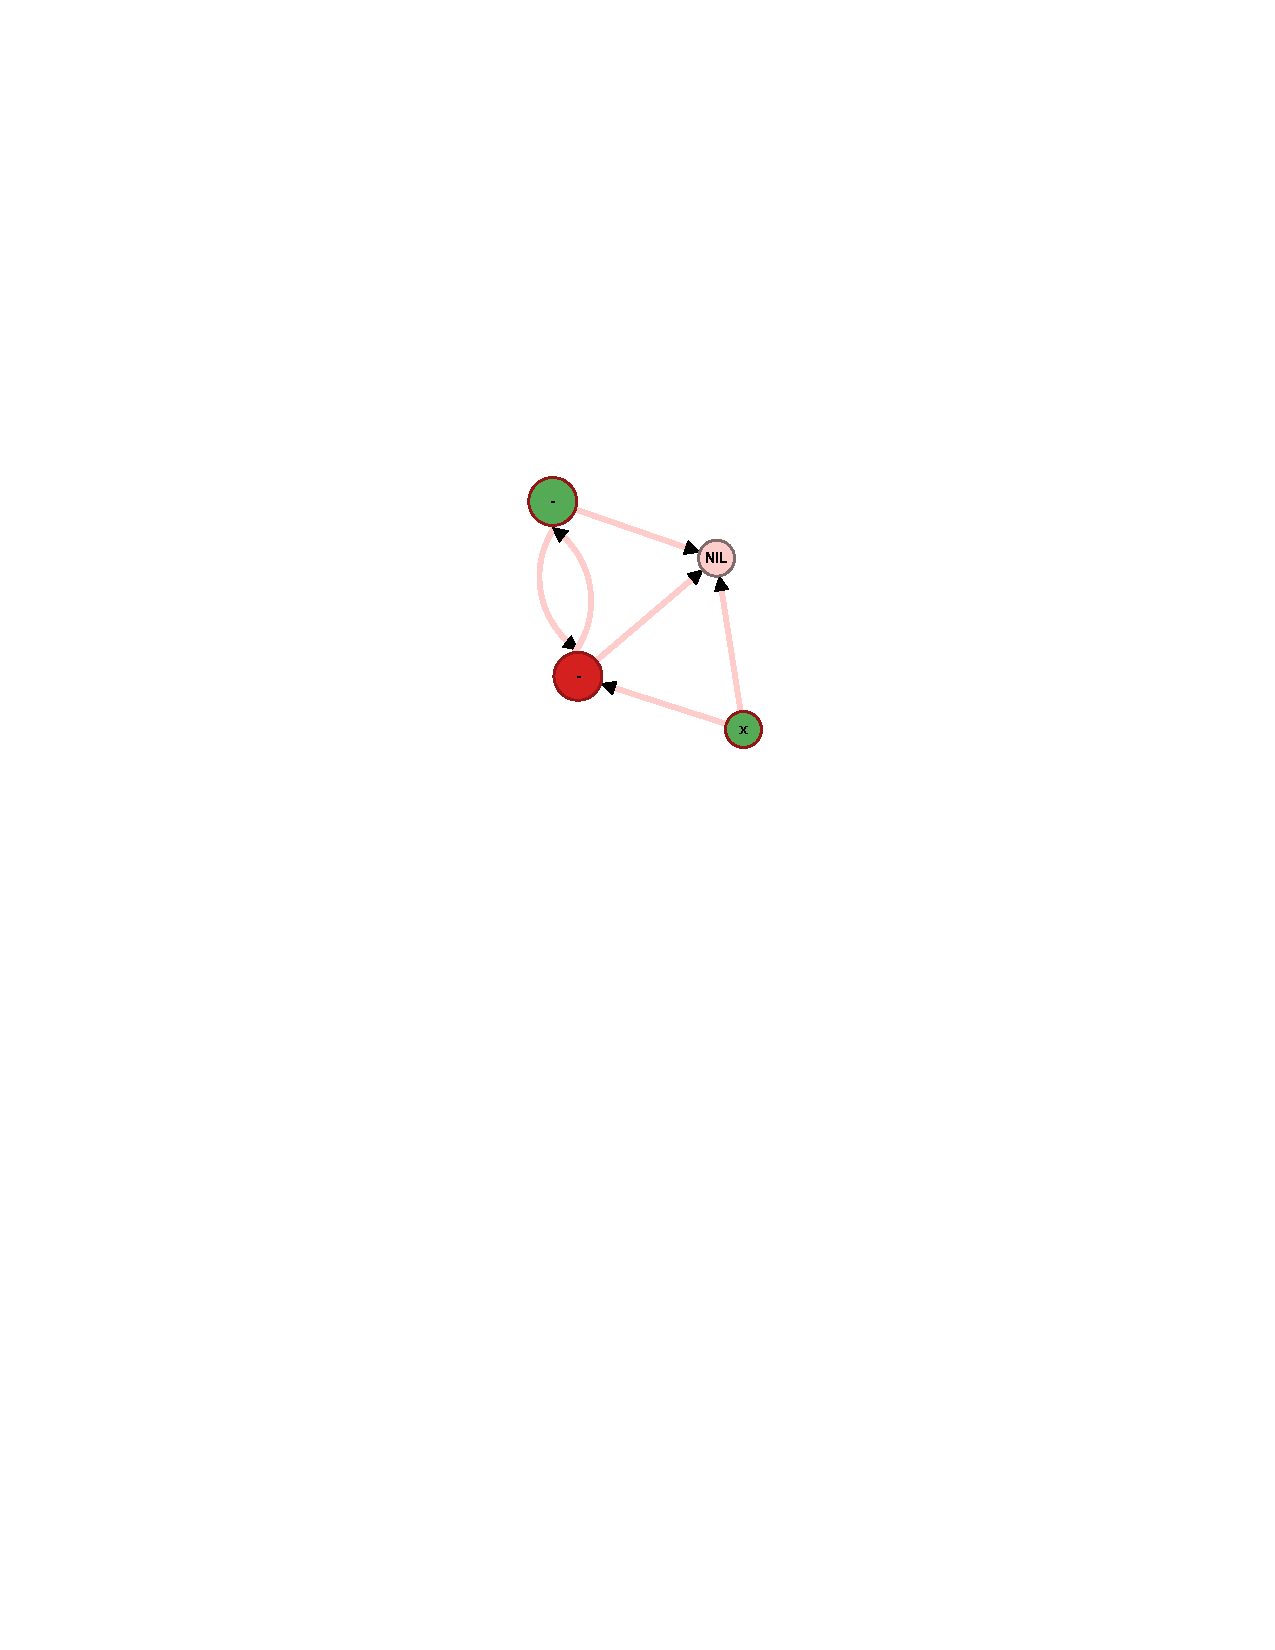
\includegraphics[width=7cm]{fig/candidate6.pdf}
  \caption{The final pattern that is accepted by the verifier. Note that this is not the strongest pattern indicating exactly the right heaps. \verifier does not need the strongest pattern, but the one that can be part of the interpolant. Too strong a pattern can lead to a lot of the vertices in the unwinding tree ending up uncovered. Too weak might mean the interpolant breaks down.}
  \label{fig:right-pattern}
\end{figure}

\section{Analyzing our Interface}
Our example in \autoref{sec:illustrating-user-interaction} gives one possible user interaction flow for the \altlistsimplified program. In this section, we present a broader discussion of the capabilities and limitations of our interface. This is important to understand what kind of programs can be handled by the heap pattern language and \verifier. They key goal of \verifier is to make it easier to provide a way to input and use unbounded heap patterns.

The visual graphical representation of heap patterns in our interface is based on \autoref{defn:pattern}. While the formalism is more difficult for humans to reason about, graphs are easier to understand. Nonetheless, the utility of our algorithm is limited by two things - (1) the expressiveness of the heap pattern language, and (2) the complexity of patterns that humans can provide. We now discuss these points in more detail.

\subsection{Expressiveness of Heap Patterns}
\label{sec:expressiveness-of-heap-patterns}
In \autoref{fig:right-pattern}, we saw a heap pattern representing an alternating list. While the pattern may not be able to perfectly capture all kinds of alternating lists, it was sufficient for the example at hand. Similarly, a pattern might also over-generalize, but it might work for a certain node in our unwinding tree. This is a great feature of interpolant-based techniques, where as long as our interpolant is able to label an error node unreachable, it is sufficient and nodes don't need to be labeled with the strongest possible labels. Whether or not a pattern is sufficient depends significantly on the requirements of the underlying verification algorithm and the property to be proved. In this section, we demonstrate some examples of heap patterns that can represent some interesting shape properties. Notice that our current implementation only supports nodes that have a single pointer field. In the future, we would like to support nodes with multiple pointer fields, which would allow us to deal with structures such as doubly linked lists, trees, and even other shapes that are less common.

We now demonstrate some interesting patten graphs, some of which are part of the SV-COMP \cite{sv-comp} benchmarks.
% https://github.com/sosy-lab/sv-benchmarks/tree/svcomp15/c/list-properties

\subsubsection{Reachability}
A list where a certain pointer is always reachable from the start

\subsubsection{Cyclic List}
A little unclear how, but we'll see. Think of automata.

\subsubsection{Inverted Tree}
The pattern will be too general, but might work

\subsubsection{Two-part List}
a*b*NIL

The last few examples show that several useful properties can be expressed using our framework. In the future, we would like to explore whether our heap pattern formalism has an equivalent in logics for describing heaps. At the same time, we note that \verifier itself is not strictly tied down to a single formalism, and it is possible to annotate nodes in the unwinding tree with other kinds of structures or formulas, and provide an Oracle that can work with them.

\subsection{Understandability of the Interface}
\label{sec:understandability-of-interface}
Describes the backgrounds of the users we asked to use it, and two examples for which they could work out reasonable patterns.

\subsubsection{Complexity of Patterns provided by Users}
Example users who used our interface
What they thought

\subsection{Experiments}
Need better title for this section. Describe what exists in the implementation. (This is also part of Sanjit's feedback).

Also describe what needs to be done as future work.

\section*{Summary}
In this chapter, we presented the web interface for the Oracle in \verifier - a human user. We described the interface design, and an overview of how a user would interact with the interface to provide a useful heap pattern that can be used in verification. We also discussed our overall implementation and its limitations. The next chapter presents some related work, and concludes with  our contributions and ideas for potential directions to take.

\chapter{Conclusion}
\label{ch:conclusion}

In this chapter, we briefly describe existing verification approaches, how they differ
from our oracle-guided approach, and summarize the contributions in this thesis.

\section{Related Work}
\label{sec:related-work}

\paragraph{Counterexample Guided Abstraction Refinement}
% CEGAR:
A broad class of verifiers of programs and transition systems have
been proposed that implement \emph{counterexample-example guided
  abstraction refinement (CEGAR)}~\cite{clarke03}.
%
The common structure of all of these analyses is that they maintain an
approximate model of the possible runs of a system, and refine the
model until it represents a proof of correctness by iteratively (1)
choosing a path of execution $p$ allowed by the model that, if
feasible, constitutes a property violation, (2) refuting the
feasibility of $p$, and (3) using the refutation to refine the paths
of execution allowed by the model.
% Relative Completeness of Abstraction Refinement for Software Model
% Checking: Oracle is really angelic non-determinism.
The CEGAR-based analysis that is most closely related to the
one proposed in this work is actually a \emph{theoretical} analysis
that chooses program facts from which to construct a refutation by
querying a \emph{widening Oracle}~\cite{ball02}.
%
The key property of the counterexample-guided analysis is that if there is
sequence of widenings that the Oracle can possible choose to cause the
analysis to verify a program, then the analysis will eventually verify
the program successfully.
%
Because the Oracle does not solve a distinct problem, but instead
provides values to the analysis, it can be viewed as an agent of
\emph{angelic non-determinism}~\cite{bodik10}.
% Us:
While \verifier also queries an Oracle, the Oracle solves a problem
distinct from providing values to the analysis, namely an active
learning problem over both positive \emph{and negative} example
heap graphs.

\paragraph{Predicate Abstraction}
% Predicate Abstraction:
Predicate abstraction is an abstract interpretation technique in which the abstract
domain is constructed from a given set of predicates over program variables. The concrete
states of a system are mapped to abstract states according to their evaluation under a
finite set of predicates. Automatic predicate abstraction algorithms have been designed
and implemented before for finite and for infinite state systems. Predicate abstraction
is well established in the literature \cite{ball01,henzinger02,henzinger04}. The primary
limitation with most of these techniques is that predicates in logic cannot describe
shapes.
% Us:
\verifier uses predicates to annotate heap patterns, relying on other technique to infer
these predicates beforehand. Predicate abstraction is useful to do that, although we
need more investigation into how to use it to infer the right predicates for our
technique in a directed way and efficiently.

\paragraph{Interpolation}
% Interpolation
Interpolants have been widely studied and used in model checking and software
verification. In various contexts, interpolation can be used as a substitute for image
computation, which involves quantifier elimination and is thus computationally
expensive. The idea is to replace the image with a weaker approximation that is still
strong enough to prove some property, helping to construct and inductive invariant.
Interpolant based techniques typically examine symbolic executions (finite paths)
through the program, explicitly enumerating paths and employing heuristics to avoid path
explosion \cite{albarghouthi12,heizmann10,mcmillan06,rummer13}. Some of them use other
optimizations to cover wider search spaces, or compute invariants more efficiently.
\verifier also uses the notion of interpolants applied to sequences, but specifically
for heap patterns. Existing techniques don't work for this case because they deal with
formulas that cannot desribe heaps or shapes in memory.
% Us

\paragraph{Active Learning and Inductive Synthesis}
% Active learning
Active learning has explored as yet another technique, which is particularly useful for
dealing with verification of data structures. The framework proposed in \cite{garg13}
can model quantified invariants over linear data structures, and build poly-time active
learning algorithms for them, where the learner is allowed to query the teacher with
membership and equivalence queries.
% Madhu's paper: only works on bounded tuples of lists
% Us

HERE
\cite{wenchao-thesis}
\cite{jha-arxiv15}

% You're missing several citations here. Need to cite Rahul Sharma's papers on
% data-driven invariant generation. Also would be useful to cite Wenchao's thesis
% on specification mining since it covers a lot of related work on that topic.
% Further the paper Susmit and I wrote on a Theory of Formal Synthesis
% via Inductive Learning, that generalizes active learning and query-based
% learning to the oracle-guided inductive synthesis framework. A broader
% discussion of the role of learning in synthesis is given in my Proc. IEEE paper.
% Would be good to expand this section to give this broader view. Sagiv et al's
% PLDI 2016 paper on the Ivy system would also come here.

\paragraph{Shape Analysis}
In program analysis, a shape analysis is a static code analysis technique that discovers
and verifies properties of linked, dynamically allocated data structures in (usually
imperative) computer programs. It has been applied to a variety of problems, including
memory safety and checking state properties. For example, proving that two data
structures cannot access the same piece of memory, or discriminating between cyclic and
acyclic lists. Separation logic \cite{calcagano11,reynolds02} is one component of
existing work on shape analysis. It extends the simple imperative programming language
with commands (not expressions) for accessing and modifying shared structures, and for
explicit allocation and deallocation of storage. Assertions are extended by introducing
a ``separating conjunction'' that asserts that its subformulas hold for disjoint parts
of the heap, and a closely related ``separating implication''. Coupled with the
inductive definition of predicates on abstract data structures, this extension permits
the concise and flexible description of structures with controlled sharing. Separation
logic is quite expressive, but the major challenge lies in finding a suitable decidable
sub-logic that is expressive enough for a given domain.

In addition to the logic approach, memory graphs have been extensively explored for
shape analysis. A parametric framework for shape analysis was presented in
\cite{sagiv02}, which can be instantiated in different ways to create shape-analysis
algorithms that provide varying degrees of efficiency and precision. It also proposed
three-valued logic structures, an idea we extensively use to model heap patterns in our
work. Symbolic Memory Graphs (SMGs) \cite{dudka13} are another effective approach,
particularly for modeling extremely low-level operations. The heap patterns used in
\verifier are partially inspired by SMGs, but work at a higher level that is more
suitable for an external Oracle, and in an interpolation-based verification framework.
% Us

\paragraph{Crowdsourcing for Formal Methods}
% Other examples of humans as oracles
The idea of using human input for assisting in computational tasks is not new. Human
computation is a paradigm for utilizing human processing power to solve problems that
computers cannot yet solve \cite{vonahn2005, quinn2011}. Formal verification techniques
are currently computationally expensive/undecidable, or require highly specialized
engineers with deep knowledge of software technology and mathematical theorem-proving
techniques, making them expensive and time-consuming. CrowdMine \cite{wenchao2012} is a
game devised for finding patterns from system traces that can suggest likely
specifications. It transforms segments of a program trace into 2D images and then
displays a small subset of them to a non-expert crowd in the form of a puzzle game,
using the input to infer program specifications. A similar idea is present in
\cite{ernst2012}, but the focus in on verifying security properties, which is achieved
by having users play a game with ball-and-pipe puzzles.

The Crowd Sourced Formal Verification (CSFV) program by
DARPA\footnote{Defense Advanced Research Projects Agency} is yet another major effort to
investigate whether large numbers of non-experts can perform formal verification faster
and more cost-effectively than conventional processes. The effort has produced some
interesting games, which are listed under Verigames \cite{verigames}.

Some other work includes \cite{pastore2013} which uses human input as test oracles for
software testing, \cite{lebras2013} which uses human domain-knowledge about a given SAT
formula to obtain backdoor variables for the SAT formula, and \cite{fast2013} which is a
system for creating, grading, and analyzing derivation assignments across arbitrary
formal domains. Thus students act as users and the system checks their assignments
(proofs) for correctness.

Crowdsourcing has been successfully used in other areas as well. Eyewire \cite{eyewire}
is a popular example. Gameplay involves 3D puzzles and advances neuroscience by helping
researchers discover how neurons connect to process visual information. Solving puzzles
actually reconstructs 3D models of neurons. Eyewire requires no scientific background to
play.
% Also proceedings of HCOMP over the last four years.
% Us

\section{Summary}
Our work can be summarized using the following key ideas:

\begin{enumerate}
  \item We extended the interpolant-based verification algorithm from \cite{mcmillan06} to work for the domain of heap-manipulating programs.
  \item We defined the heap pattern formalism for expressing sets of concrete heaps.
  \item We introduced a framework for oracle-guided synthesis of heap patterns, which allows the verification algorithm to use an external Oracle for the generalization step.
  \item We demonstrated one example of such an Oracle - a human user who is good at generalizing shapes, and can provide valuable insight to help find heap interpolants.
\end{enumerate}

Our framework is very general, in the sense that it allows for any kind of ``pattern''
formalism to be used alongside a domain expert Oracle. This provides two advantages.
Firstly, it makes it very easy to try a simple interpolation-based verification
algorithm for a new domain, where one might not have good automated techniques for
generalization, but good ``intuitive'' understanding about it. Secondly, it simplifies
plugging in different Oracles into an existing verification algorithm, allowing for
broader possible insight into the analysis. It is easy to extend this to the case of
allowing for multiple Oracles working side by side in a single analysis, providing
complementary insight into a verification problem. In the future, a theoretical analysis
of oracle-guided verification algorithms would be an interesting direction.

HERE

% Would be useful to cite the Jha and Seshia OGIS paper here, since it does
% develop first steps of a theory of inductive synthesis (but the point you make
% about doing for heap invariants is a valid one worth making).
% http://arxiv.org/abs/1505.03953


% bibliography:
\bibliographystyle{alpha}
\small
% \setlength{\bibsep}{3pt}
\bibliography{p,conf}
\end{document}
